\documentclass{article}
\usepackage[submission]{colm2026_conference}

\usepackage{microtype}
\usepackage{hyperref}
\usepackage{url}
\usepackage{booktabs}
\usepackage{graphicx}
\usepackage{amsfonts}
\usepackage{amsmath}
\usepackage{xcolor}
\usepackage{subcaption}
\usepackage{float}
\usepackage{tabularx}
\usepackage{multirow}

\usepackage{lineno}

\definecolor{darkblue}{rgb}{0, 0, 0.5}
\hypersetup{colorlinks=true, citecolor=darkblue, linkcolor=darkblue, urlcolor=darkblue}

\title{Where's the Plan? Pinpointing Latent Planning in Language Models}

\author{Author 1 \\ Stanford University \And Author 2 \\ Stanford University}

\newcommand{\fix}{\marginpar{FIX}}
\newcommand{\new}{\marginpar{NEW}}

\begin{document}

\ifcolmsubmission
\linenumbers
\fi

\maketitle

\begin{abstract}
    Prior work establishes that language models exhibit evidence of latent planning, but does not address $\textit{where and how}$ planning mechanisms form. We introduce the notion of $\textit{planning site formation}$ and investigate it across Qwen3, Gemma-3, and Llama-3 model families at multiple scales using lightweight mechanistic methods on poem generation tasks. Probing reveals substantial cross-model and cross-scale diversity in planning-compatible representations at the newline token. Activation patching reveals that planning-compatible representations do not imply causal planning behavior. We find that only Gemma-3-27B forms a causally active planning site at the newline via an information routing handoff, implemented by a sparse set of attention heads. All other models condition on the last word token throughout generation despite exhibiting planning-compatible representations, suggesting planning site formation is a distinct emergent phenomenon, not a general property of capable language models. Unlike transcoders or steering vectors, our activation patching methods require orders of magnitude less compute and data, making them a more scalable framework for studying latent planning across model families.
\end{abstract}


\section{Introduction}

Autoregressive language models generate text one token at a time, yet routinely produce outputs requiring long-range structural coherence. Rhyming couplets, for example, require that tokens generated late in the sequence stand in a precise phonological relation to a stimulus word from much earlier. This raises a natural question: do models form internal representations of future outputs that causally shape generation, entirely invisible to behavioral evaluation? We call this \textit{latent planning}. Unlike chain-of-thought reasoning~\citep{wei2022chain}, where intermediate steps are directly observable, latent planning occurs entirely within a model's hidden activations. If models are planning in ways invisible to external observers, standard behavioral evaluations may systematically underestimate this capacity---making it both a scientific and a safety-relevant problem~\citep{pfau2024dots,hao2024coconut}.

Neural networks trained on next-step prediction can develop internal planning representations in structured domains. McGrath et al.~\citeyearpar{mcgrath22} find that chess concepts emerge in AlphaZero's internal layers; Li et al.~\citeyearpar{li24} and Nanda et al.~\citeyearpar{nanda23} show that transformers trained on Othello develop linear, causally manipulable board representations; and Jenner et al.~\citeyearpar{jenner24} provide mechanistic evidence of learned look-ahead in a chess-playing network. These results motivate the question of whether language models elicit analogous mechanisms during open-ended generation. Prior work on large language models establishes that planning-compatible information exists in some models~\citep{maar2026whatsplanmetricsimplicit,hanna2026latent,dong2025emergentresponseplanningllms,pochinkov2025parascopeslanguagemodelsactivations}, but does not address a more specific question: \textit{where exactly does planning information reside during the forward pass, and does it move?} We call this \textbf{planning site formation}.

Investigating planning sites rigorously requires both encoding evidence (what information is present) and causal evidence (what information is used). Probes assess what is encoded in hidden states~\citep{hewitt19,burns24}, but sufficiently flexible probes can achieve high accuracy by memorizing labels rather than reflecting genuine representations~\citep{hewitt19}. Causal tools such as activation patching~\citep{meng23,wang2022ioi} and steering vectors~\citep{turner2023activation,arditi2024refusal} are needed to establish that encoded information actually influences downstream generation. The most expressive existing approach---training transcoders~\citep{transcoders} to build feature circuits~\citep{sparsefeaturecircuits,ameisen2025circuittracing}---provides fine-grained circuit analysis, but requires substantial compute (effectively a second training run), has so far been applied only to closed-source models such as Claude Haiku 3.5~\citep{anthropic-bio}, and does not straightforwardly scale to new open-source architectures. Work by \citet{maar2026whatsplanmetricsimplicit} uses steering vector interventions and finds most open-source models up to 30B parameters keep their planning sites at the last word token; a transcoder-based analysis by \citet{anthropic-bio} on Claude Haiku 3.5 finds evidence of a planning site migrating to the newline. These results motivate a scalable framework for studying planning site formation across model architectures and scales.

In this paper, we define two notions for surfacing evidence of latent planning: the weaker notion of \textit{planning-compatible representations} (detectable via probing) and the stricter notion of \textit{causally active planning sites} (established via activation patching). Using only linear probing and activation patching---requiring no transcoder training and far less data than steering vector approaches---we investigate planning site formation across three open-source model families at multiple scales (up to 32B parameters).

Probing reveals that planning-compatible representations emerge at the newline token with scale across all three families, yet their strength and layer profile vary substantially across architectures. Activation patching reveals a sharp dissociation: only Gemma-3-27B forms a causally active planning site at the newline, exhibiting an information routing handoff in which causal influence migrates from the last word token to the newline around layer 30. All other models---including all Qwen3 sizes up to 32B and all Llama-3 sizes up to 8B---condition on the last word token throughout generation despite encoding planning-compatible representations at the newline. We further localize the handoff in Gemma-3-27B to a sparse set of five attention heads spanning layers 28--34, identified via attention weight ranking and simultaneous head patching. This suggests that planning site formation is a distinct emergent phenomenon tied to specific model scale and architecture, rather than a general consequence of strong planning-compatible representations.

% \paragraph{Contributions (TBD)}
% \begin{enumerate}
% \item The first causal investigation of \textit{planning site formation} across multiple
%   architectures and scales, using a barebones minimal activation patching intervention to determine whether and where the
%   causal locus of rhyme planning information migrates during the forward pass.
% \item Discovery and characterization of the \textit{information routing handoff} in models like
%   Gemma-3-27B: last-word causal effect drops and newline causal effect rises
%   simultaneously around layer 30, confirmed by both patching and steering.
% \item A within-family replication of the encoding/deployment dissociation across all
%   tested Qwen3 scales: planning-compatible representations exist at the newline, yet
%   causal effect is near-zero at every scale.
% \item Independent cross-paper corroboration: Maar et al.'s steering sweep identifies
%   the same Gemma-3-27B outlier pattern, providing convergent evidence under a different
%   method.
% \end{enumerate}


\section{Setup and Notation}
\label{sec:2}
In this paper, we study rhyming couplet generation as an example of latent planning. 
A rhyming couplet is a two-line poem where the last word of the first line, denoted $r_1$, rhymes with the last word of the second line, denoted $r_2$. 
We task language models to complete rhyming couplets, (i.e., given context containing $r_1$, generate a completion where $r_2$ rhymes with $r_1$). For example, 
\begin{align*}
    \text{Prompt: }& \texttt{A rhyming couplet:\textbackslash nShe felt a sudden sense of fright,\textbackslash n} \\
    \text{Completion: }& \texttt{and hoped that dawn would end the night.\textbackslash n}
\end{align*}
where $r_1 = \texttt{fright}$ and $r_2 = \texttt{night}$.

Consider an autoregressive transformer language model with $L$ layers and hidden dimension $d$. 
Let $\mathbf{h}_{\ell,i} \in \mathbb{R}^d$ denote the hidden state vector after the $\ell$-th transformer block at position $i$. 
We adopt a relative positioning scheme centered around the newline token $\verb|\n|$ ending the first line of the couplet. 
We refer to this token as being at position 0, with position $i$ referring to an offset of $i$ behind/ahead of the newline. 

% See Appendix \ref{sec:model-config} for subtle details regarding differences in tokenization between models.

We say $(i, \ell)$ contains a \textit{planning-compatible representation} if the generated $r_2$ can be decoded from  $\mathbf{h}_{\ell,i}$ bia probing substantially better at position $i$ than at other positions. 
This signals information about the future token and/or rhyme scheme is disproportionally \emph{encoded} at the location $(i, \ell)$ compared to other hidden states.
As a stricter definition, we say $(i, \ell)$ is a \textit{causally active planning site} if replacing $\mathbf{h}_{\ell,i}$ during generation with the hidden state from a run targeting a different rhyme substantially redirects output toward that rhyme. 
This shows that rhyme information located at $(i, \ell)$ is causally used in generation. 


% Rhyme evaluation uses the CMU Pronouncing
% Dictionary~\citep{cmu}. We study Gemma-3~\citep{gemma3} and Qwen3~\citep{qwen3} at
% multiple scales (1B through 27B and 32B respectively) and Llama~\citep{llama3} up to 70B.
% See Appendix~\ref{sec:model-config} for architectural details.
% We synthetically generate rhyming couplets using Claude Sonnet 4.6~\citep{sonnet46}, and truncate them to use as model prompts. 


\section{Probing for Planning-Compatible Representations}
\label{sec:probing}
To investigate planning-compatible representations, we train linear probes to predict future tokens from hidden states. 
Let $\mathcal V$ be the vocabulary (set of all tokens) and $\Delta \mathcal V$ the probability simplex over $\mathcal V$. 
Each linear probe is a parameterized function $f_{(W,b)}(\mathbf{h}): \mathbb{R}^d \to \Delta \mathcal V$ where $f_{(W,b)}(\mathbf{h}) = \text{softmax}(W\mathbf{h} + \mathbf{b})$.
Probes are trained by minimizing cross-entropy loss. Probe parameters are optimized with AdamW~\citep{adamw} with learning rate $10^{-4}$, weight decay $10^{-3}$, batch size 32, for 10 epochs. 

\subsection{Probing general text as a negative control}
\label{sec:probe-general}

We first verify that planning-compatible representations are task-specific and do not occur in general text generation. 
We randomly sample 1,200 (1,000 train, 200 validation) token sequences from The Pile~\citep{thepile}, greedily sample model completions while storing activations to build the probe training dataset. 
For each layer $\ell$ and various \textit{look-ahead distance} $k$, we train a linear probe to predict the generated token at position $i+k$ from $\mathbf{h}_{\ell,i}$. 
We compare against a baseline unigram model (trained on the corpus of all model competions) to ensure probes are learning more than just token frequencies. 

\begin{figure}[h]
    \centering
    \begin{subfigure}{0.325\linewidth}
        \centering
        \subcaption[]{Qwen3-32B}
        
\includegraphics[width=\linewidth]{media/results-probe/qwen-top5.png}
    \end{subfigure}
    \begin{subfigure}{0.325\linewidth}
        \centering
        \subcaption[]{Gemma-3-27B}
        
\includegraphics[width=\linewidth]{media/results-probe/gemma-top5.png}
    \end{subfigure}
    \begin{subfigure}{0.325\linewidth}
        \centering
        \subcaption[]{Llama-3.1-70B}
        
\includegraphics[width=\linewidth]{media/results-probe/gemma-top5.png}
    \end{subfigure}
    \caption{Top-5 accuracy of linear probes predicting $k$ tokens ahead in general text.}
    \label{fig:probe-results}
\end{figure}

We find probe accuracy degrades monotonically with $k$ and falls to baseline by $k=8$ across all
layers and both models (Figure~\ref{fig:probe-results}), confirming that
planning-compatible representations are not a generic property of the residual stream. 
This provides a negative control establishing that probe signal in Section~\ref{sec:probe-couplets} is significant.

\subsection{Probing rhyming couplets}
\label{sec:probe-couplets}
For rhyming couplet generation, we first synthetically generate 1,200 (1,000 train, 200 validation) rhyming couplets with Claude Sonnet 4.6 \citep{sonnet46}, strategically prompting for diversity of topics and rhyme schemes. 
We truncate the second line of each couplet, then greedily sample model completions for the second line, storing activations to build the probe training dataset. 
We train probes to predict the rhyming token $r_2$ from $\mathbf{h}_{\ell,i}$ (Figure~\ref{fig:poem-diagram}), evaluating on raw accuracy and rhyme accuracy (as determined by the CMU Pronouncing Dictionary \citep{cmu}) across layers and positions.
The comparison is between probes trained on activations at the newline position ($i=0$) and subsequent positions ($i > 0$). 
If a model constructs a planning-compatible representation at the newline before generation begins, the $i=0$ probe should substantially outperform $i>0$ probes. We also probe on hidden states at the last word token position, \footnote{Position $i=-2$ in Gemma and $i=-1$ in Qwen and Llama (see Appendix \ref{sec:model-config})}, which we expect to perform well since the last word directly decides the rhyme scheme of the couplet.

\begin{figure}[h]
    \centering
    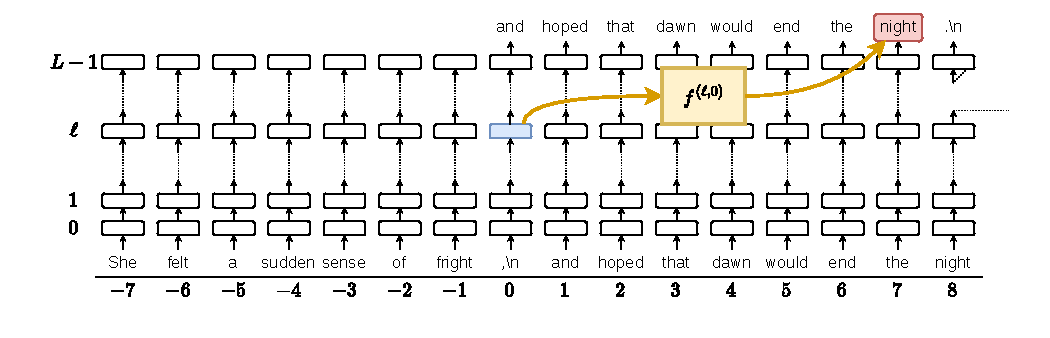
\includegraphics[width=\linewidth]{media/diagrams/probe-diagram.pdf}
    \caption{A linear probe $f^{(\ell,0)}$ trained to predict the rhyming token from
    activations at the newline position ($i=0$).}
    \label{fig:poem-diagram}
\end{figure}

\begin{figure}[h]
    \centering
    \begin{subfigure}{0.325\linewidth}
        \centering
        \subcaption[]{Qwen3-32B (Top-5 Acc.)}
        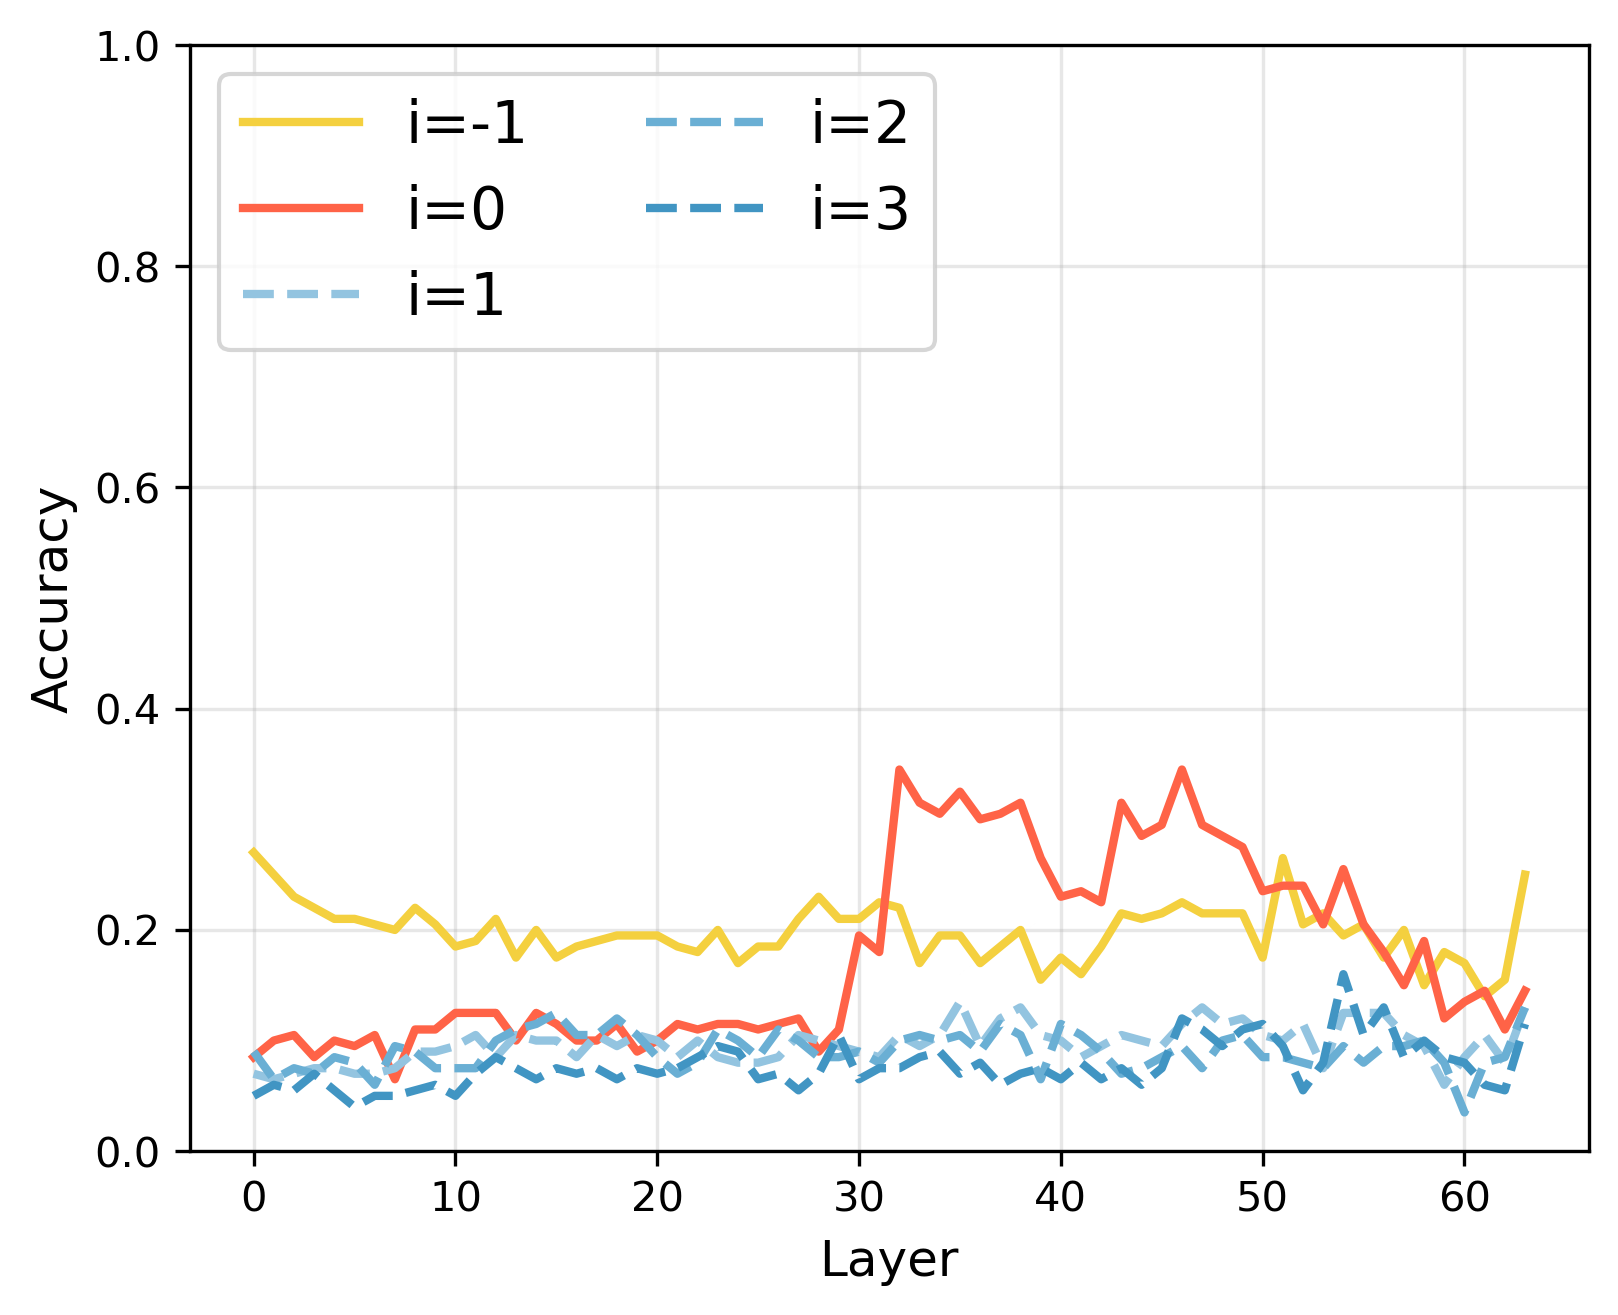
\includegraphics[width=\linewidth]{media/results-poem/qwen-top5.png}
    \end{subfigure}
    \begin{subfigure}{0.325\linewidth}
        \centering
        \subcaption[]{Gemma-3-27B (Top-5 Acc.)}
        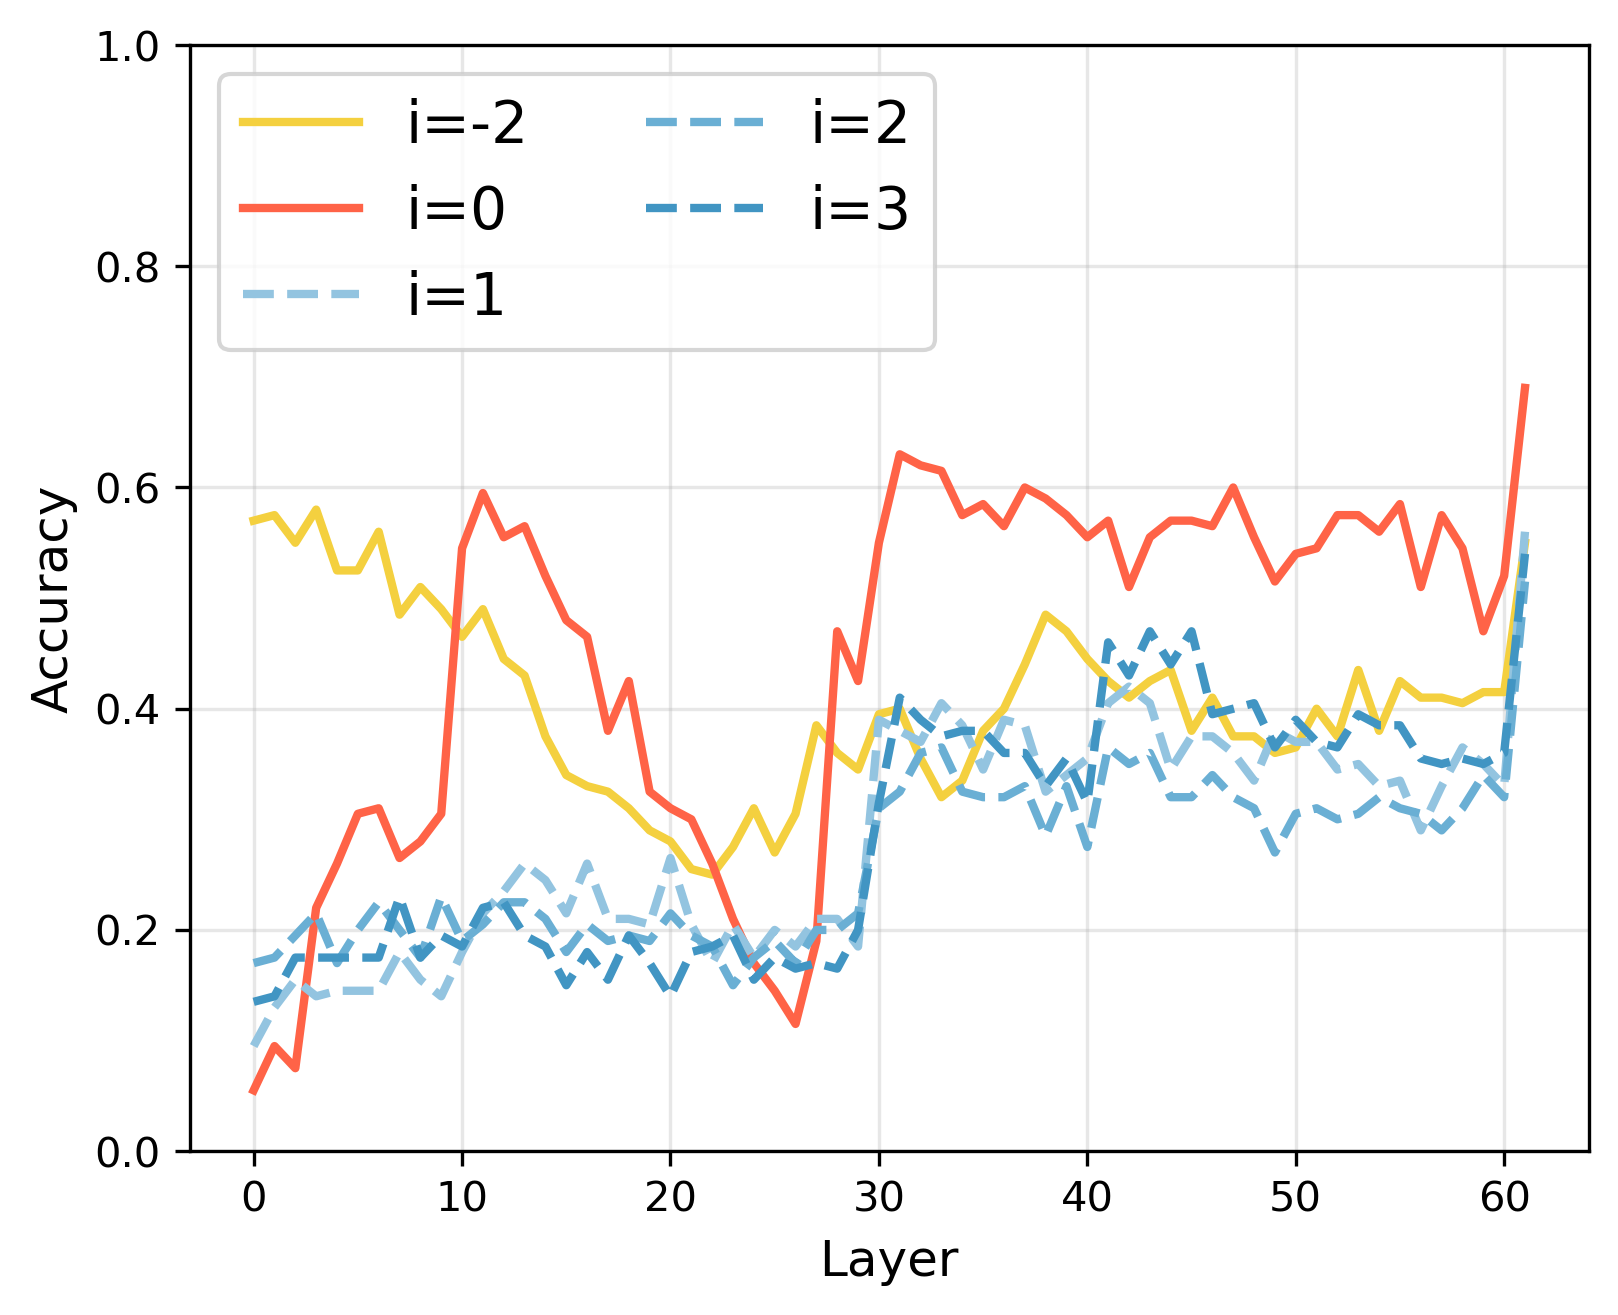
\includegraphics[width=\linewidth]{media/results-poem/gemma-top5.png}
    \end{subfigure}
    \begin{subfigure}{0.325\linewidth}
        \centering
        \subcaption[]{Llama-3.1-70B (Top-5 Acc.)}
        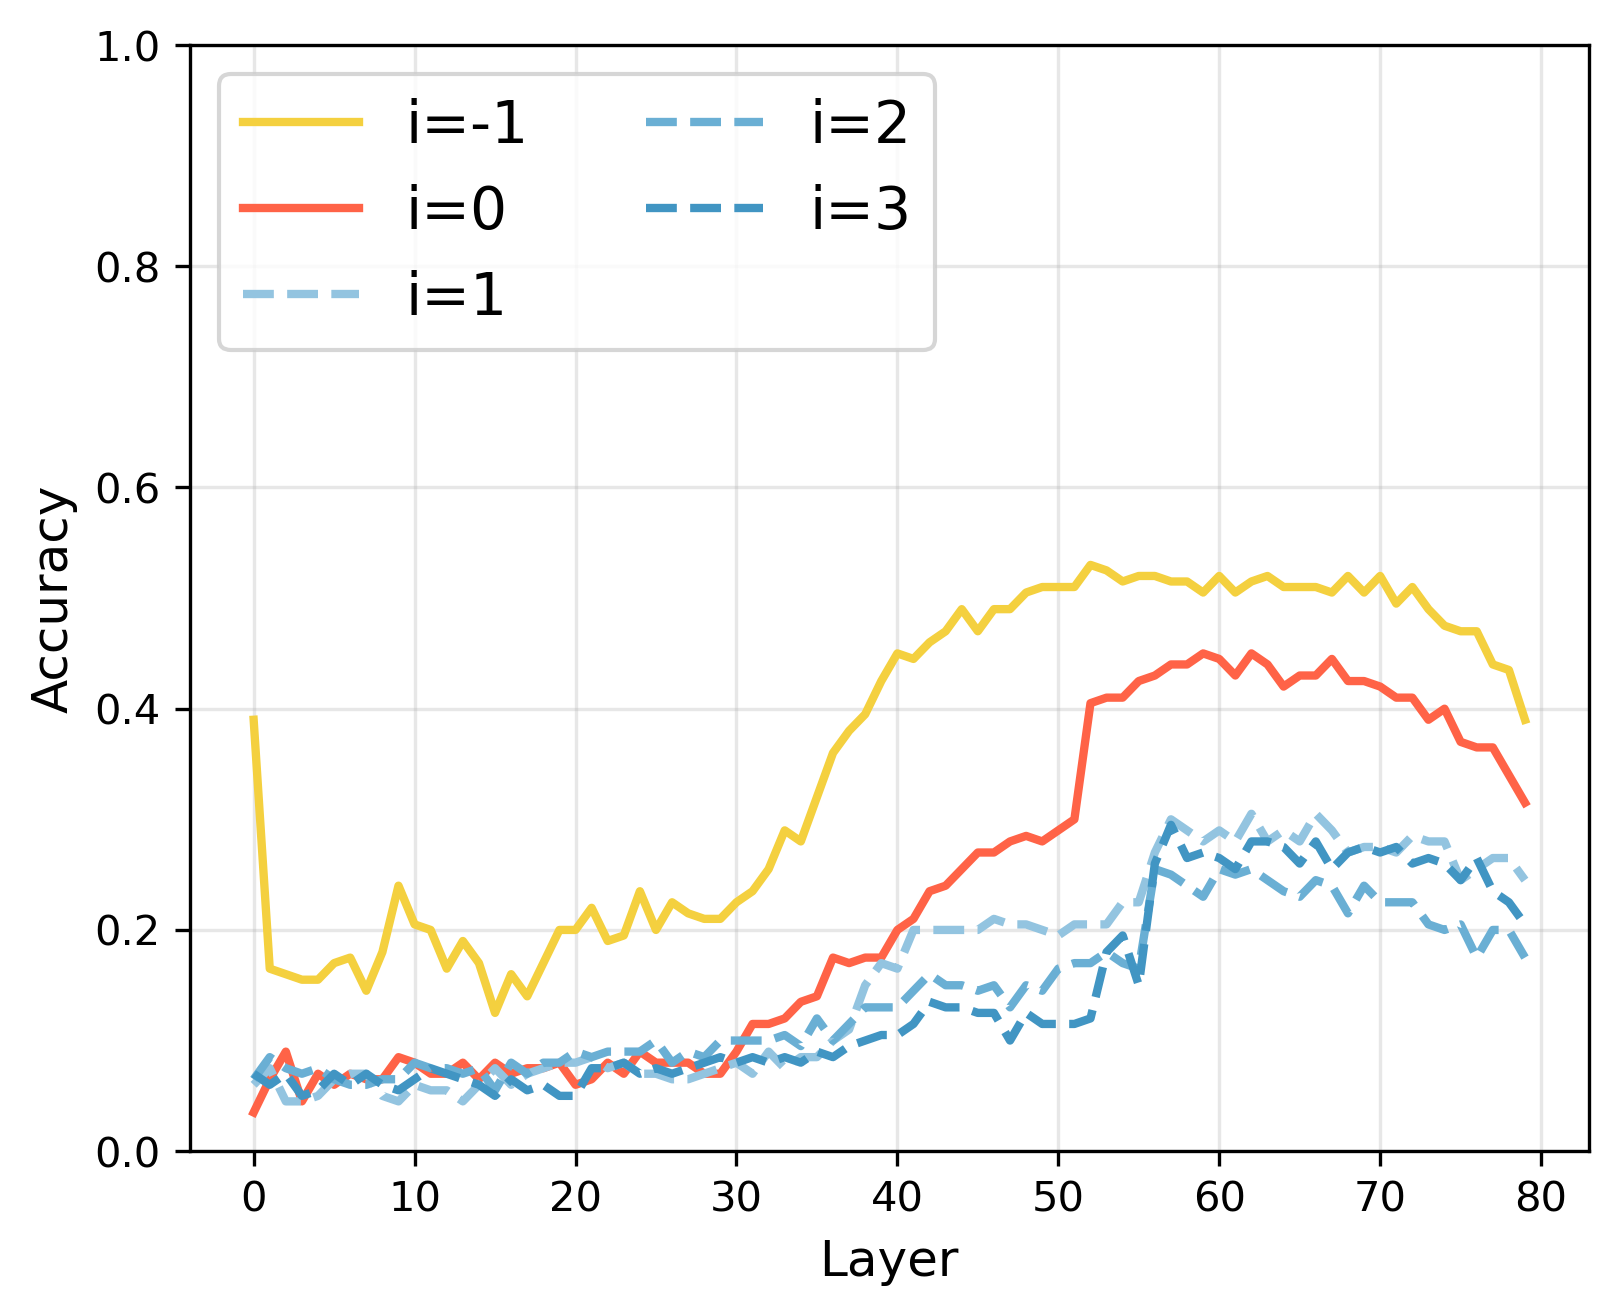
\includegraphics[width=\linewidth]{media/results-poem/llama-top5.png}
    \end{subfigure}
    \centering
    \begin{subfigure}{0.325\linewidth}
        \centering
        \subcaption[]{Qwen3-32B (Rhyme Acc.)}
        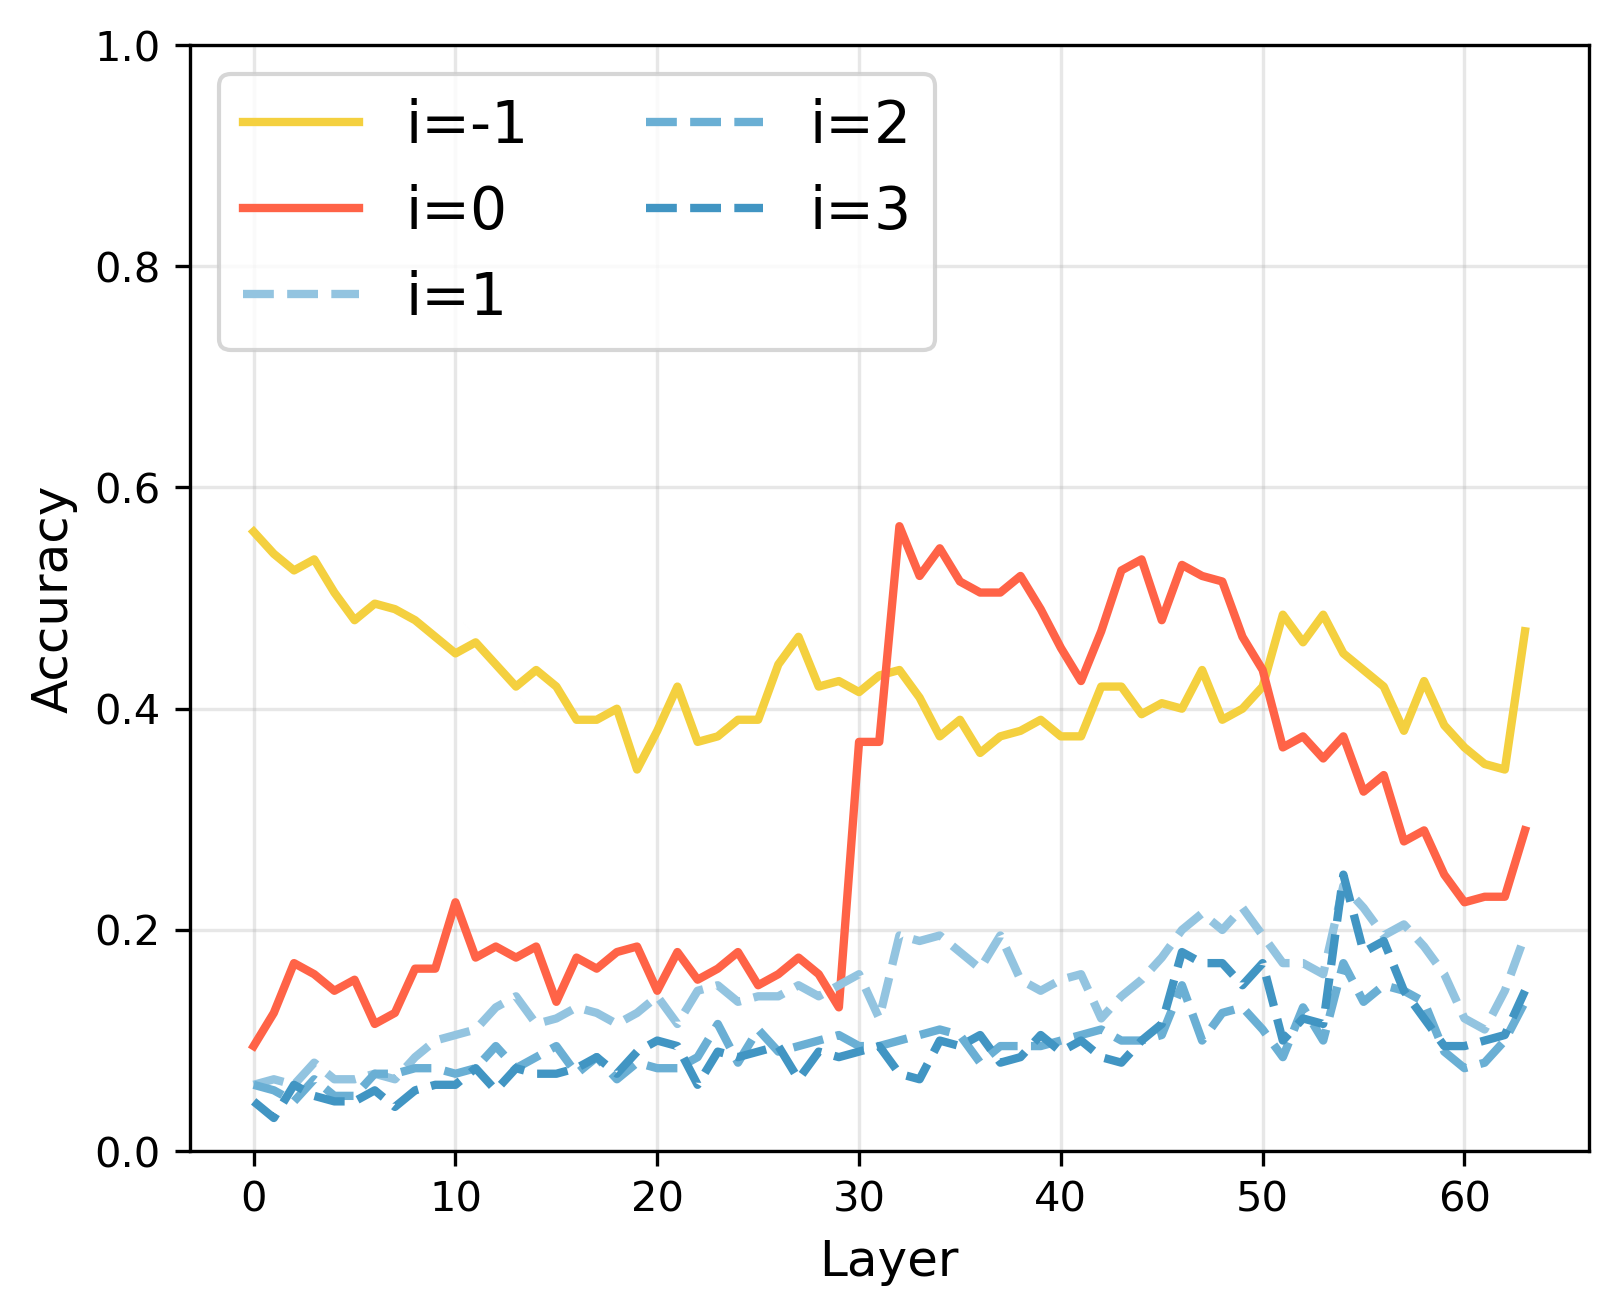
\includegraphics[width=\linewidth]{media/results-poem/qwen-rhyme1.png}
    \end{subfigure}
    \begin{subfigure}{0.325\linewidth}
        \centering
        \subcaption[]{Gemma-3-27B (Rhyme Acc.)}
        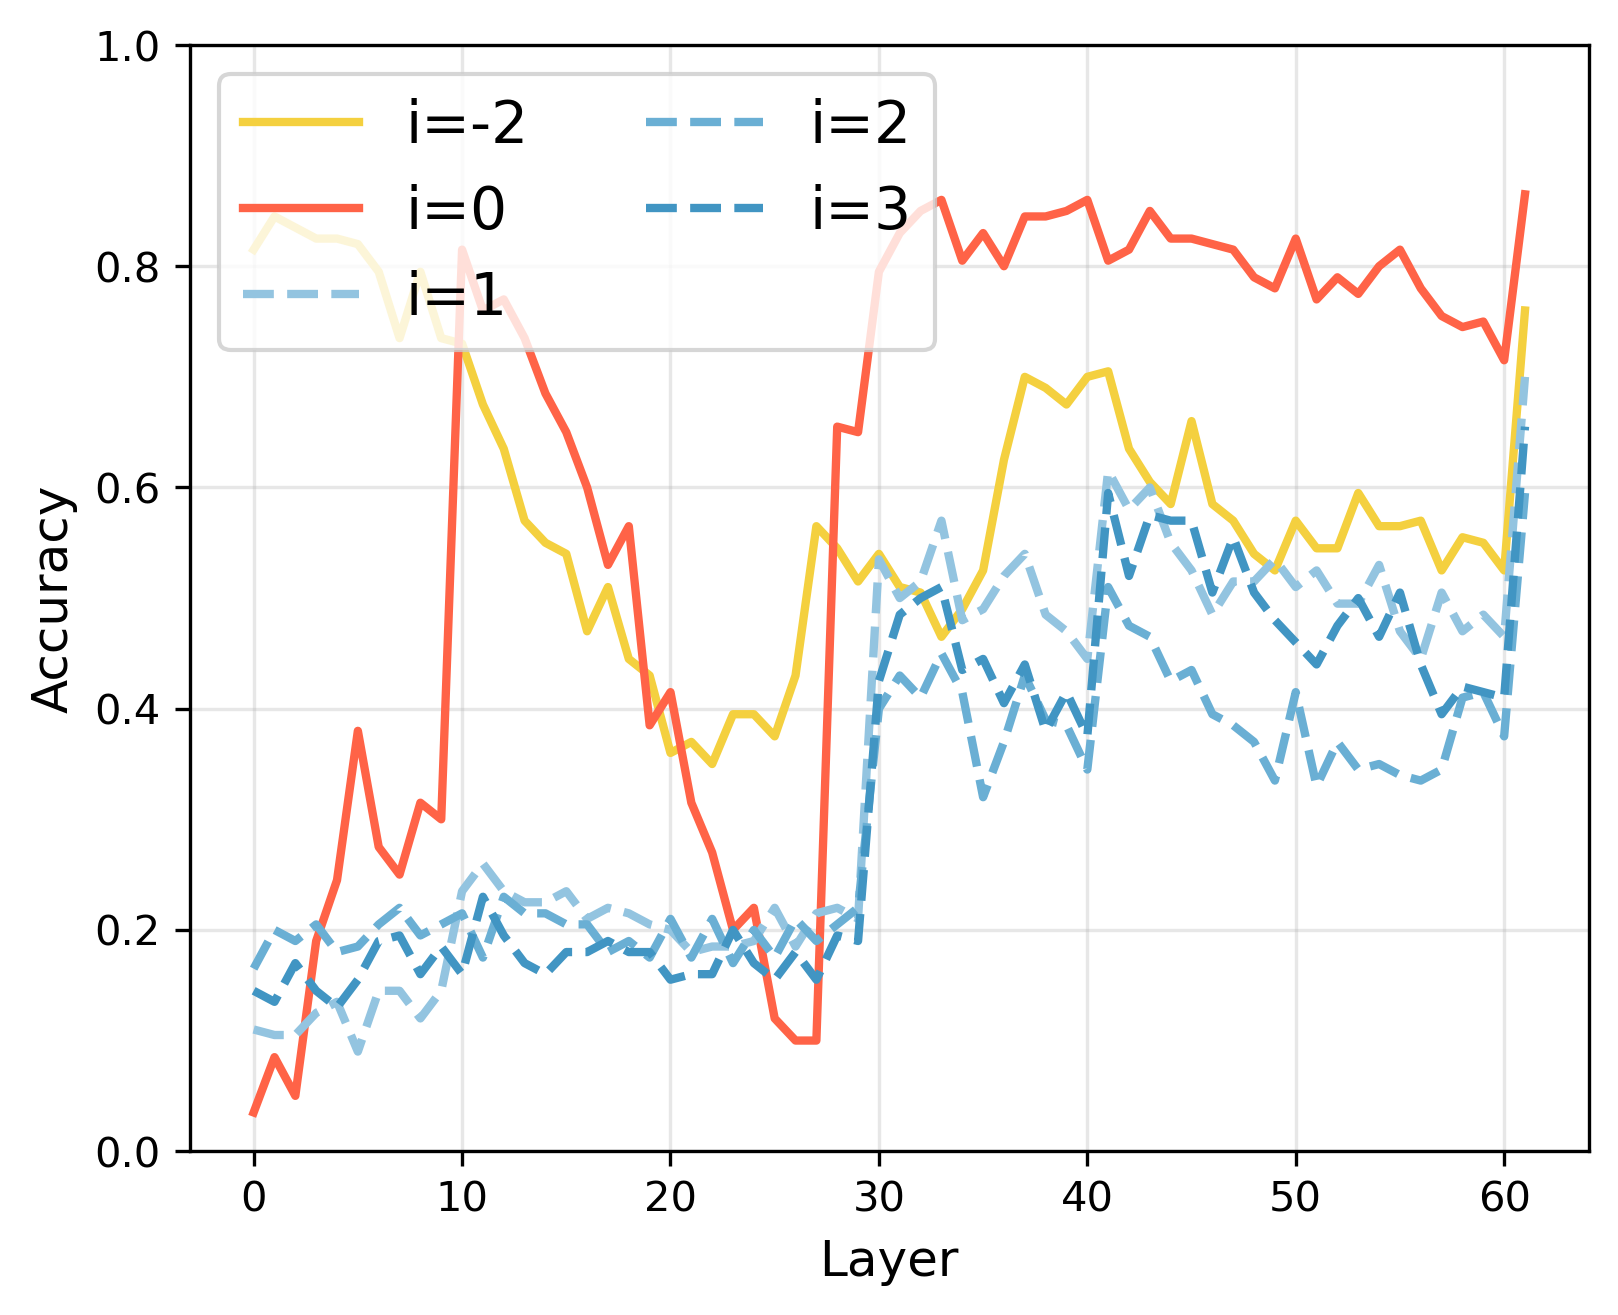
\includegraphics[width=\linewidth]{media/results-poem/gemma-rhyme1.png}
    \end{subfigure}
    \begin{subfigure}{0.325\linewidth}
        \centering
        \subcaption[]{Llama-3.1-70B (Rhyme Acc.)}
        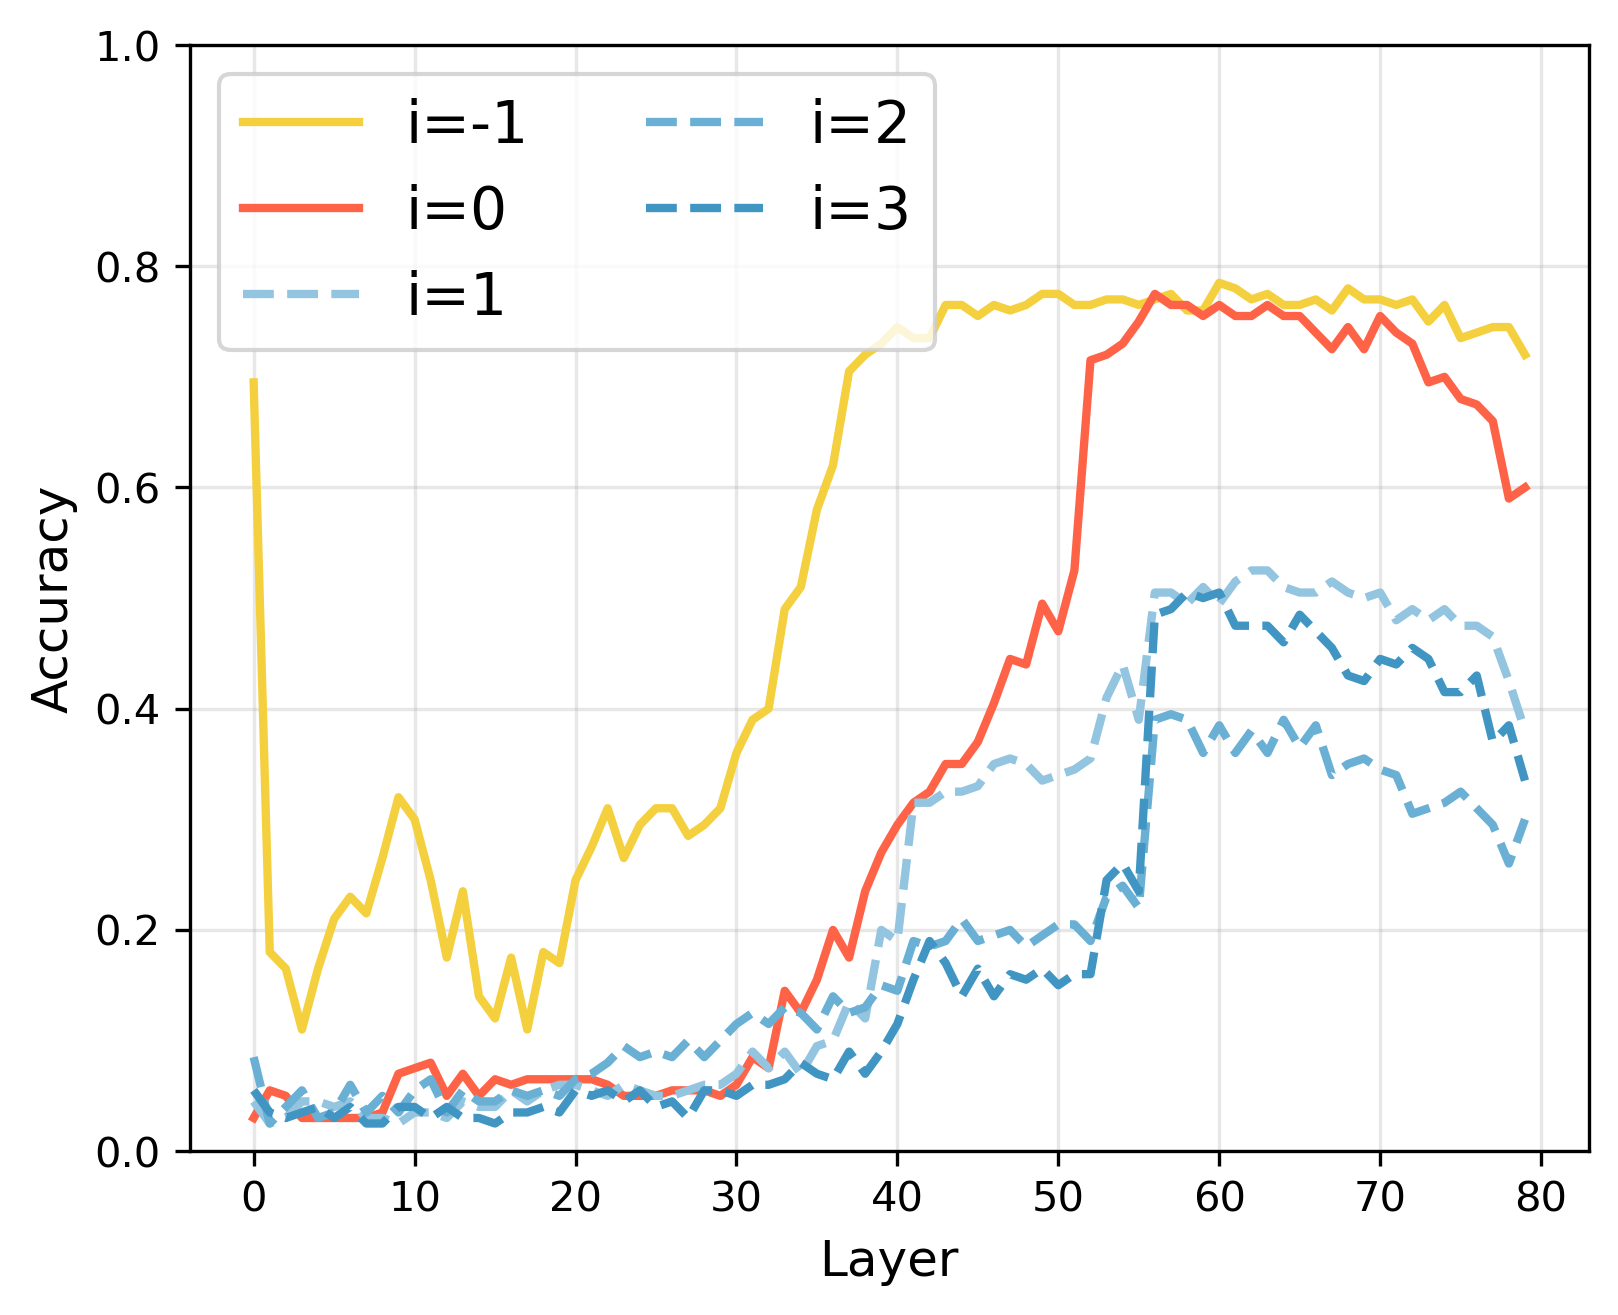
\includegraphics[width=\linewidth]{media/results-poem/llama-rhyme1.png}
    \end{subfigure}
    \caption{Top-5 and rhyme accuracy of linear probes trained to predict $r_2$ from hidden states at various layers and positions.}
    \label{fig:poem-results}
\end{figure}

% Both models show elevated $i=0$ probe signal in middle layers.
%     Gemma-3-27B shows two peaks (layers 10--20 and 30--40); Qwen3-32B shows one
%     sustained elevation (layers 30--50). Whether these representations are causally
%     active is determined in Section~\ref{sec:patching}.

First, we observe much higher accuracies probing to predict $r_2$ compared to general text. 
On average, the generated $r_2$ is 8 tokens ahead of the newline token (the last context token), and we observe much greater accuracy for the $i=0$ probes compared to the $k=8$ probes on general text. 
This suggests models selectively construct planning-compatible representations in response to the structural demands of rhyming couplet generation.

More significantly, we find evidence that these representations are concentrated in the last word and newline positions in certain layers (Figure \ref{fig:poem-results}). This is demonstrated by the large differences in accuracy from the $i\leq0$ probes compared to the $i>0$ probes, which contradicts the pattern found while probing in general text that increasing look-ahead distance decreases probe accuracy. 

Notably, probes trained on activations at the last word position all peak in accuracy early and decrease later, consistent with lexical identity of $r_1$ being encoded from the earliest layers.

However, it is nontrivial that probes trained at the newline position also do perform well, hinting at the possibility of latent planning occuring at the newline token. Notably, probes trained at both positions vastly differ in the shape of their accuracy curves between layers compared to probes at $i>0$, which seem to follow a similar shape throughout. This suggests that the newline and last word tokens undergo qualitatively different computations across layers, consistent with these positions playing a specialized role in encoding rhyme-relevant information rather than passively accumulating context like later positions.

Replicating this experiment on smaller Qwen, Gemma, and Llama models reveals these planning-compatible representations at the newline token emerge with scale. For each model, we record the largest accuracy gap across layers between probes trained at the newline token and probes trained at the next token. We find that this accuracy gap increases significantly with scale (Figure \ref{fig:poem-scaling}), suggesting that planning-compatible representations are an emergent property.


\begin{figure}[h]
    \centering
    \begin{subfigure}{0.49\linewidth}
        \centering
        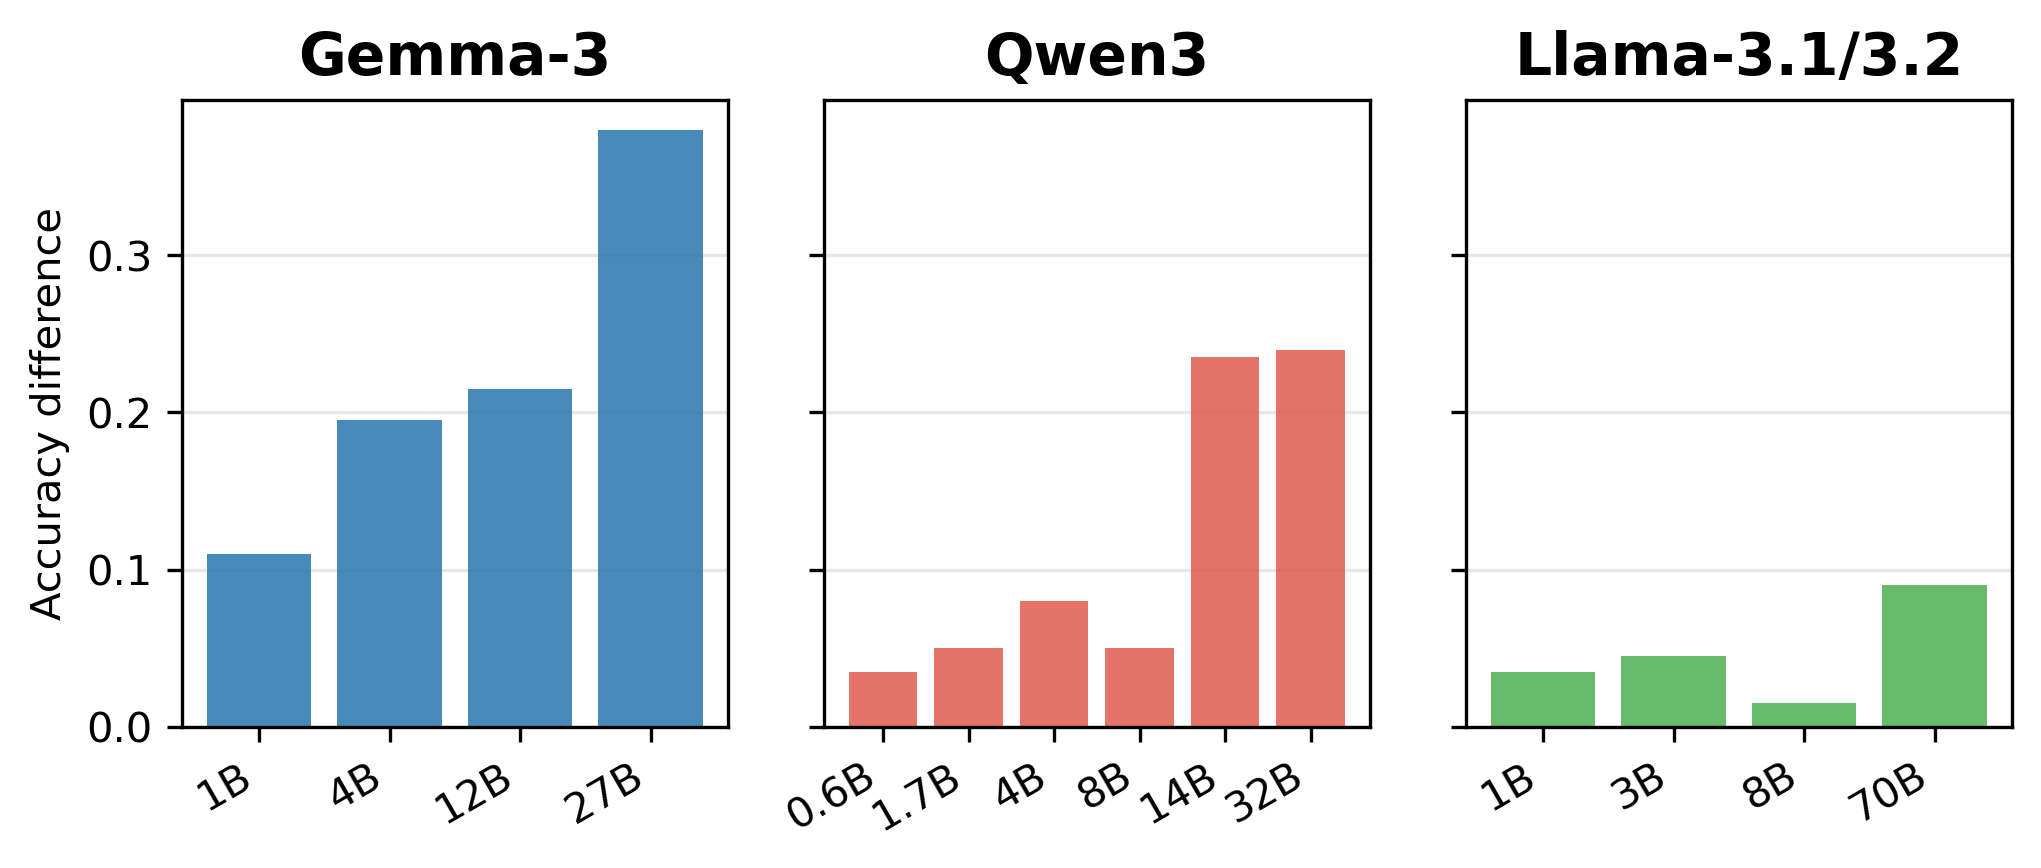
\includegraphics[width=\linewidth]{media/results-poem/scaling-top5.png}
        \subcaption[]{Top-5 Accuracy Difference}
    \end{subfigure}
    \begin{subfigure}{0.49\linewidth}
        \centering
        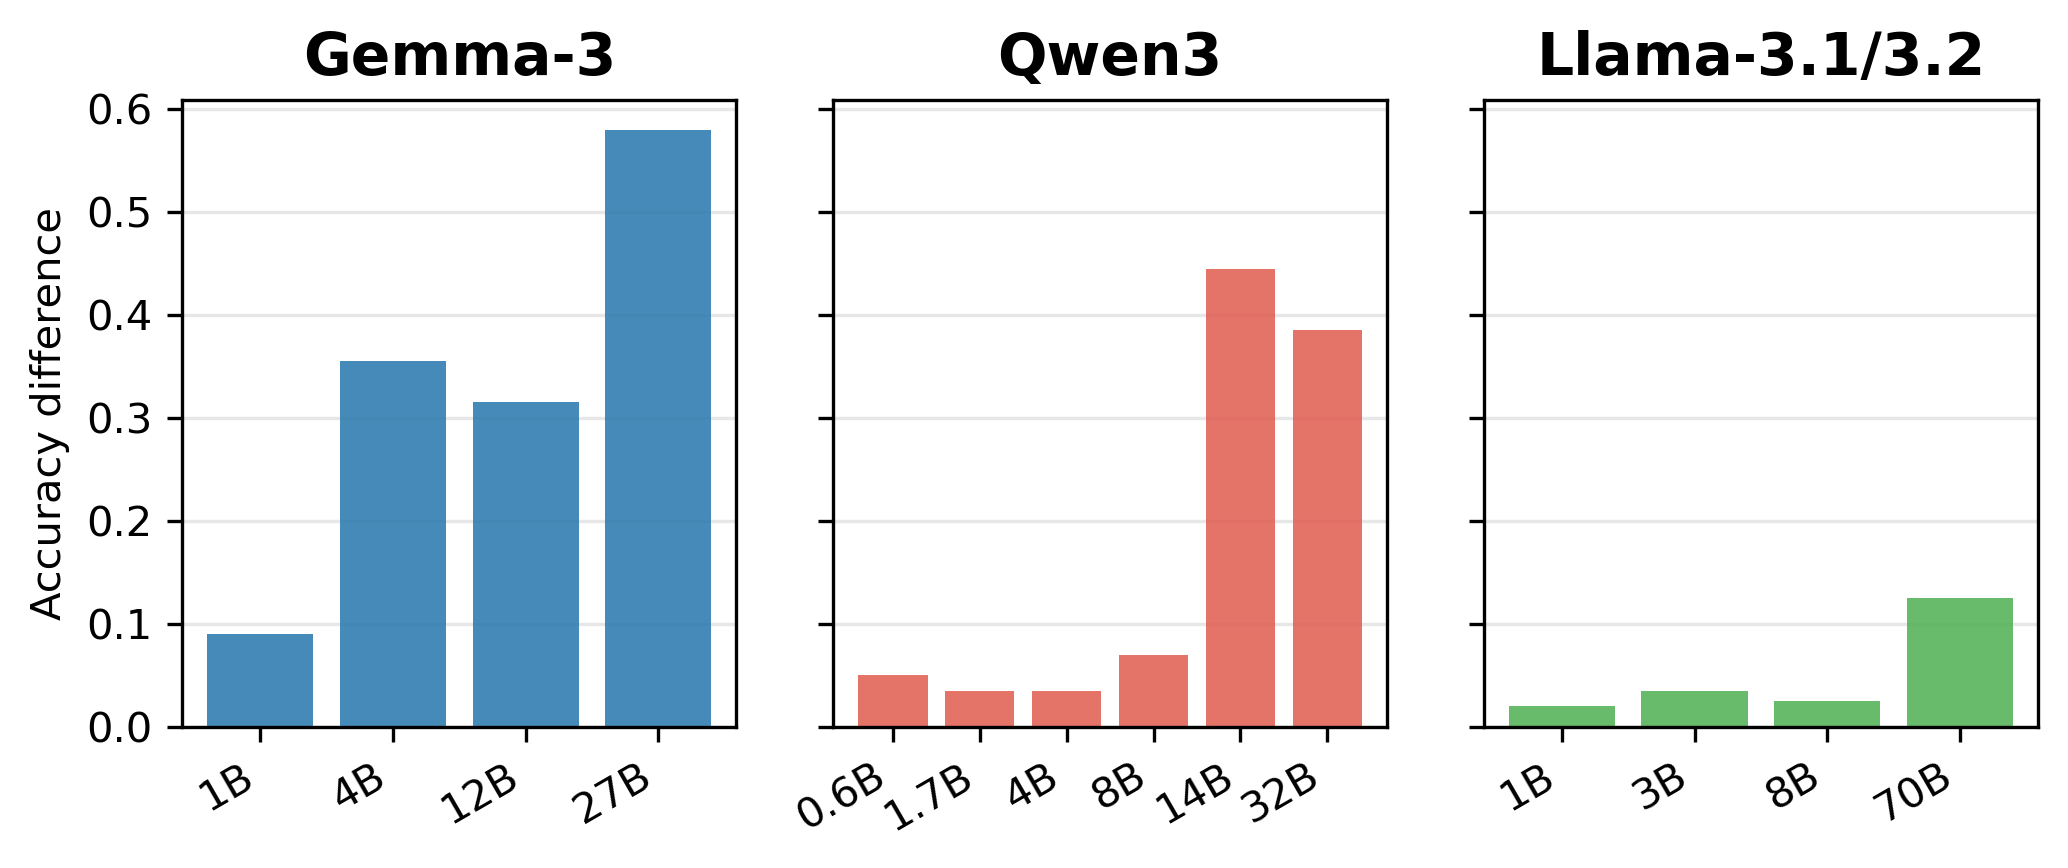
\includegraphics[width=\linewidth]{media/results-poem/scaling-rhyme1.png}
        \subcaption[]{Rhyme Accuracy Difference}
    \end{subfigure}
    \caption{Maximum accuracy difference across layers between probes trained on position 0 (newline activations) and position 1.}
    \label{fig:poem-scaling}
\end{figure}


\subsection{Discussion and limitations of probing}
\label{sec:probe-discussion}

The probing results reveal substantial cross-model and cross-scale diversity in planning-compatible representations at both the last word and newline positions. However, several alternative explanations warrant consideration. 

First, the elevated newline probe accuracy could reflect passive attention accumulation rather than active planning: if models attend strongly from the newline to the rhyme word in the first line, the newline hidden state will encode rhyme-relevant information even without any downstream computation reading it out during generation. Also, rhyme accuracy as a metric is also imperfect, as the CMU Pronouncing Dictionary does not capture all valid rhymes, potentially underestimating probe performance inconsistently across rhyme families. Additionally, though we prompted Claude to generate couplets with diverse subjects and rhyme schemes, the resulting dataset may still carry nontrivial distributional biases that could inflate probe accuracy in ways difficult to detect or control for.

These considerations highlight two fundamental limitations of probing as a method. First, high probe accuracy establishes that rhyme-relevant information is linearly decodable at a position, but cannot establish that this information causally drives generation. Second, probe accuracy is sensitive to the distribution of the training data, meaning results could partially reflect dataset artifacts rather than genuine planning representations.

Activation patching addresses both limitations directly: by intervening on specific hidden states during generation and measuring the causal effect on output, it neither requires a probe training distribution nor conflates passive encoding with active deployment. We turn to activation patching in the next section to resolve these ambiguities.



\section{Patching for Causally Active Planning Sites}
\label{sec:patching}

\begin{figure}[h]
    \centering
    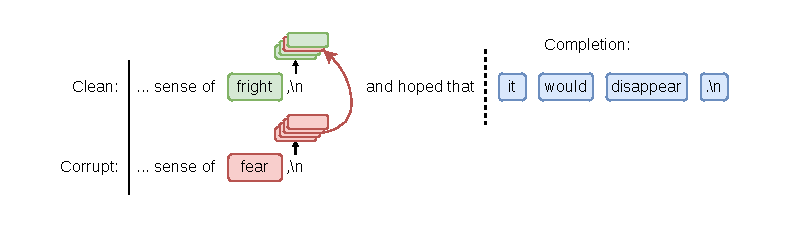
\includegraphics[width=\linewidth]{media/diagrams/patch2-diagram.pdf}
    \caption{Patch caption.}
    \label{fig:patch-diagram}
\end{figure}

While probing reveals that future token information is \textit{encoded} in hidden states, it does not establish that this information is \textit{causally used} by the model. In this section, we further investigate latent planning in rhyming couplet generation by employing intervention methods to test for causal influence directly. Given a prompt $\mathbf{x}^{(c)}$ whose first line naturally leads to a \textit{clean} rhyme family $\mathcal{R}^{(c)}$, we intervene on the model's activations at various positions and investigate whether the generation of the second line shifts toward a different \textit{corrupted} rhyme family $\mathcal{R}^{(r)}$. A successful intervention on a specific layer $\ell$ and position $i$ provides causal evidence that information at $\mathbf{h}_{\ell, i}$ is causally involved in the model's latent planning downstream.

\begin{figure}[h]
    \centering
    \begin{subfigure}{\linewidth}
        \centering
        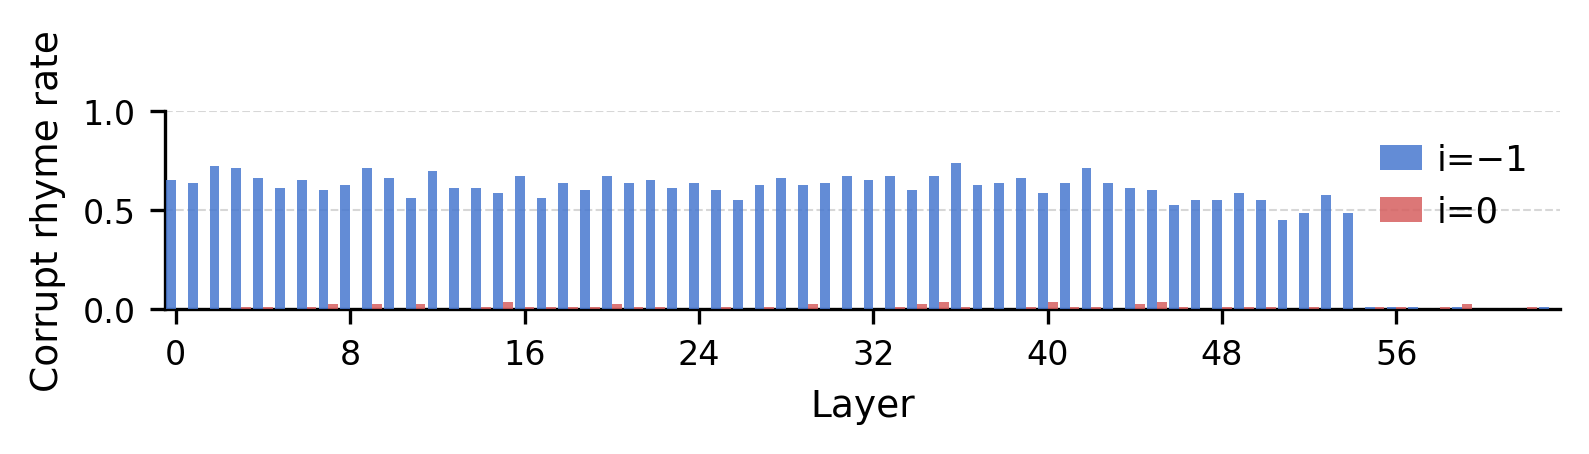
\includegraphics[width=\linewidth]{media/results-patching/patching_qwen3_32b.png}
        \caption{Qwen3-32B.}
        \label{fig:patch-qwen}
    \end{subfigure}
    \begin{subfigure}{\linewidth}
        \centering
        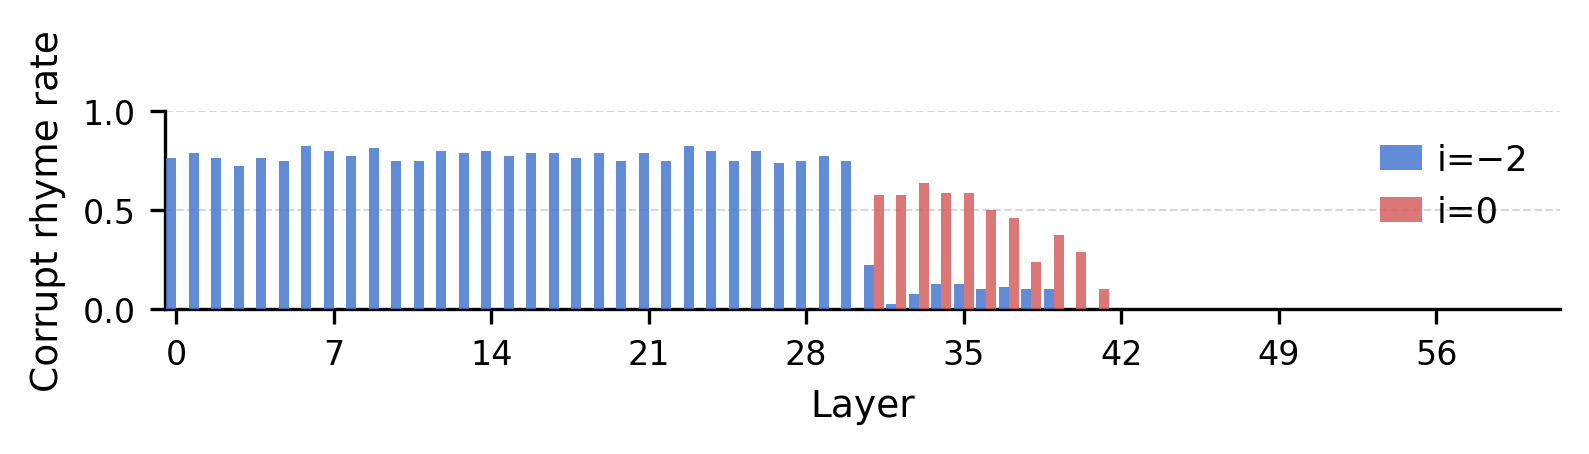
\includegraphics[width=\linewidth]{media/results-patching/patching_gemma3_27b.png}
        \caption{Gemma-3-27B.}
        \label{fig:patch-gemma}
    \end{subfigure}
    \begin{subfigure}{\linewidth}
        \centering
        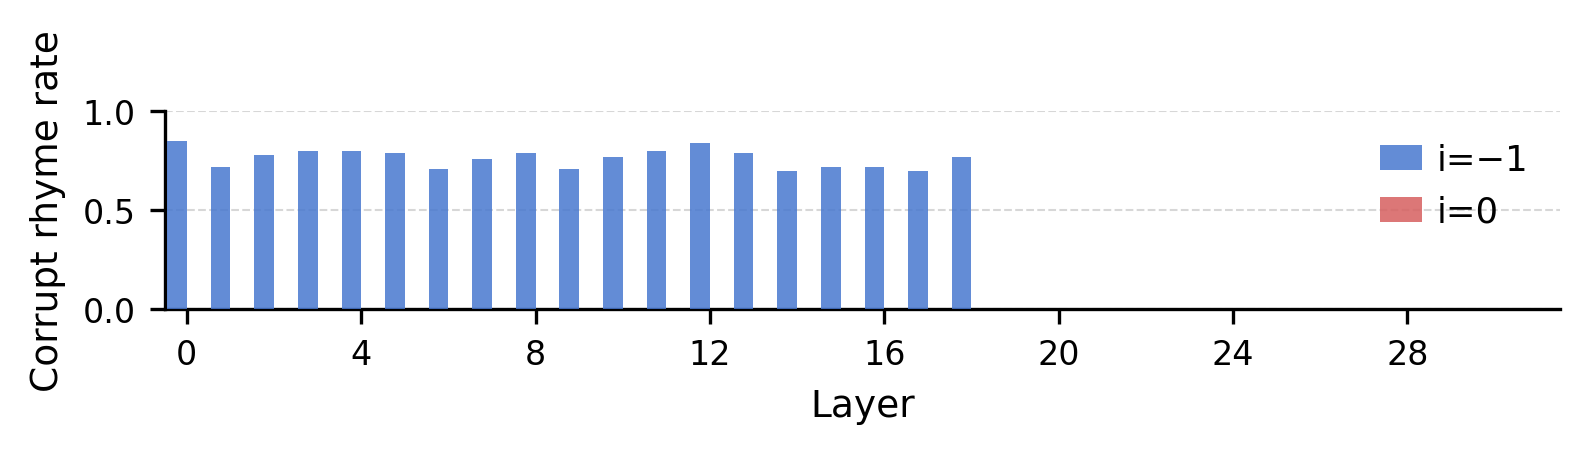
\includegraphics[width=\linewidth]{media/results-patching/patching_llama_8b.png}
        \caption{Llama-3.1-8B.}
        \label{fig:patch-llama}
    \end{subfigure}
    \caption{Per-layer activation patching at the last word token and newline ($i=0$) for the largest model in each family. Full results for all model sizes are in Appendix~\ref{sec:additional-patching-details}.}
    \label{fig:patch-results}
\end{figure}

We apply activation patching at two positions: the last word token (position $i=-1$ in Qwen3 and Llama-3, $i=-2$ in Gemma-3 due to its tokenization of the line-ending comma; see Appendix~\ref{sec:model-config}) and the newline token ($i=0$), sweeping across all layers individually. For each layer, we report the corrupt rhyme rate averaged over 20 prompt pairs. Figure~\ref{fig:patch-results} shows results for the largest model in each family.

In Gemma-3-27B (Figure~\ref{fig:patch-gemma}), last-word patching is highly effective in early layers but drops sharply around layer 30, while newline patching rises simultaneously to a peak corrupt rhyme rate of ${\sim}0.63$ at layers 33--35. This crossover---which we term the \textit{representational handoff}---is the mechanistic signature of \textit{planning site formation}: the causal locus migrates from the last word token to the newline, which becomes the primary read-out site for the phonological constraint. In contrast, Qwen3-32B (Figure~\ref{fig:patch-qwen}) and Llama-3.1-8B (Figure~\ref{fig:patch-llama}) show uniformly high last-word patching and near-zero newline patching across all layers, indicating that no such migration occurs. These models condition on the last word token throughout generation. Per-layer results for all model sizes within each family are provided in Appendix~\ref{sec:additional-patching-details}.

\subsection{Localizing the Handoff to a Sparse Set of Attention Heads}
\label{sec:head-patching}

Having established that the planning site forms at the newline token in Gemma-3-27B, we ask whether the information routing handoff can be attributed to a small, identifiable set of attention heads. Single-head patching at the newline---replacing one head's output at a time within the planning layer range (layers 27--45)---produced no measurable signal for any individual head, suggesting the representation is not localized to a single circuit element. Exhaustive combinatorial search over head subsets is computationally infeasible, so we instead use attention weights as a proxy for which heads are most likely to route rhyme information from the last word token to the newline.

Specifically, we extract the attention weight from the newline token ($i=0$) to the last word token ($i=-2$) for each head in layers 27--45 of both clean and corrupt forward passes, and rank heads by this weight. Figure~\ref{fig:topk-heads}a shows the resulting heatmap: attention to $i=-2$ is highly concentrated, with three heads---layer 30 head 4 (weight ${\approx}0.99$), layer 28 head 14 (${\approx}0.97$), and layer 28 head 15 (${\approx}0.95$)---attending almost exclusively to the last word token from the newline. A second cluster of heads in layers 28--36 shows moderate attention weights (0.35--0.55).

We then patch the top-$k$ heads by attention weight simultaneously, replacing their outputs at the newline position with those from the corrupt forward pass, and measure the resulting corrupt rhyme rate. Figure~\ref{fig:topk-heads}b shows that $k=1,2,3$ produce near-zero corrupt rhyme rates (0.00, 0.05, and 0.12, respectively), indicating that even the three highest-attending heads are individually and jointly insufficient to carry the full phonological signal. At $k=5$, the corrupt rhyme rate jumps to ${\sim}0.46$---comparable to the peak achieved by full residual stream patching at the best single layer (${\sim}0.63$, shown as a dashed reference). Adding further heads ($k=10$) does not improve the rate, which plateaus at ${\sim}0.44$.

These results reveal a sparse but distributed implementation of the handoff: a set of five attention heads spanning layers 28--34 collectively account for the bulk of the rhyme information routed to the newline, while individual heads or smaller subsets are insufficient. The top five heads by attention weight are (layer 30, head 4), (layer 28, head 14), (layer 28, head 15), (layer 30, head 5), and (layer 28, head 29). We also verified that patching top-$k$ MLP layer outputs at the same position yields zero corrupt rhyme rate for all $k$, confirming that the handoff is mediated by attention rather than feed-forward computation.

\begin{figure}[h]
    \centering
    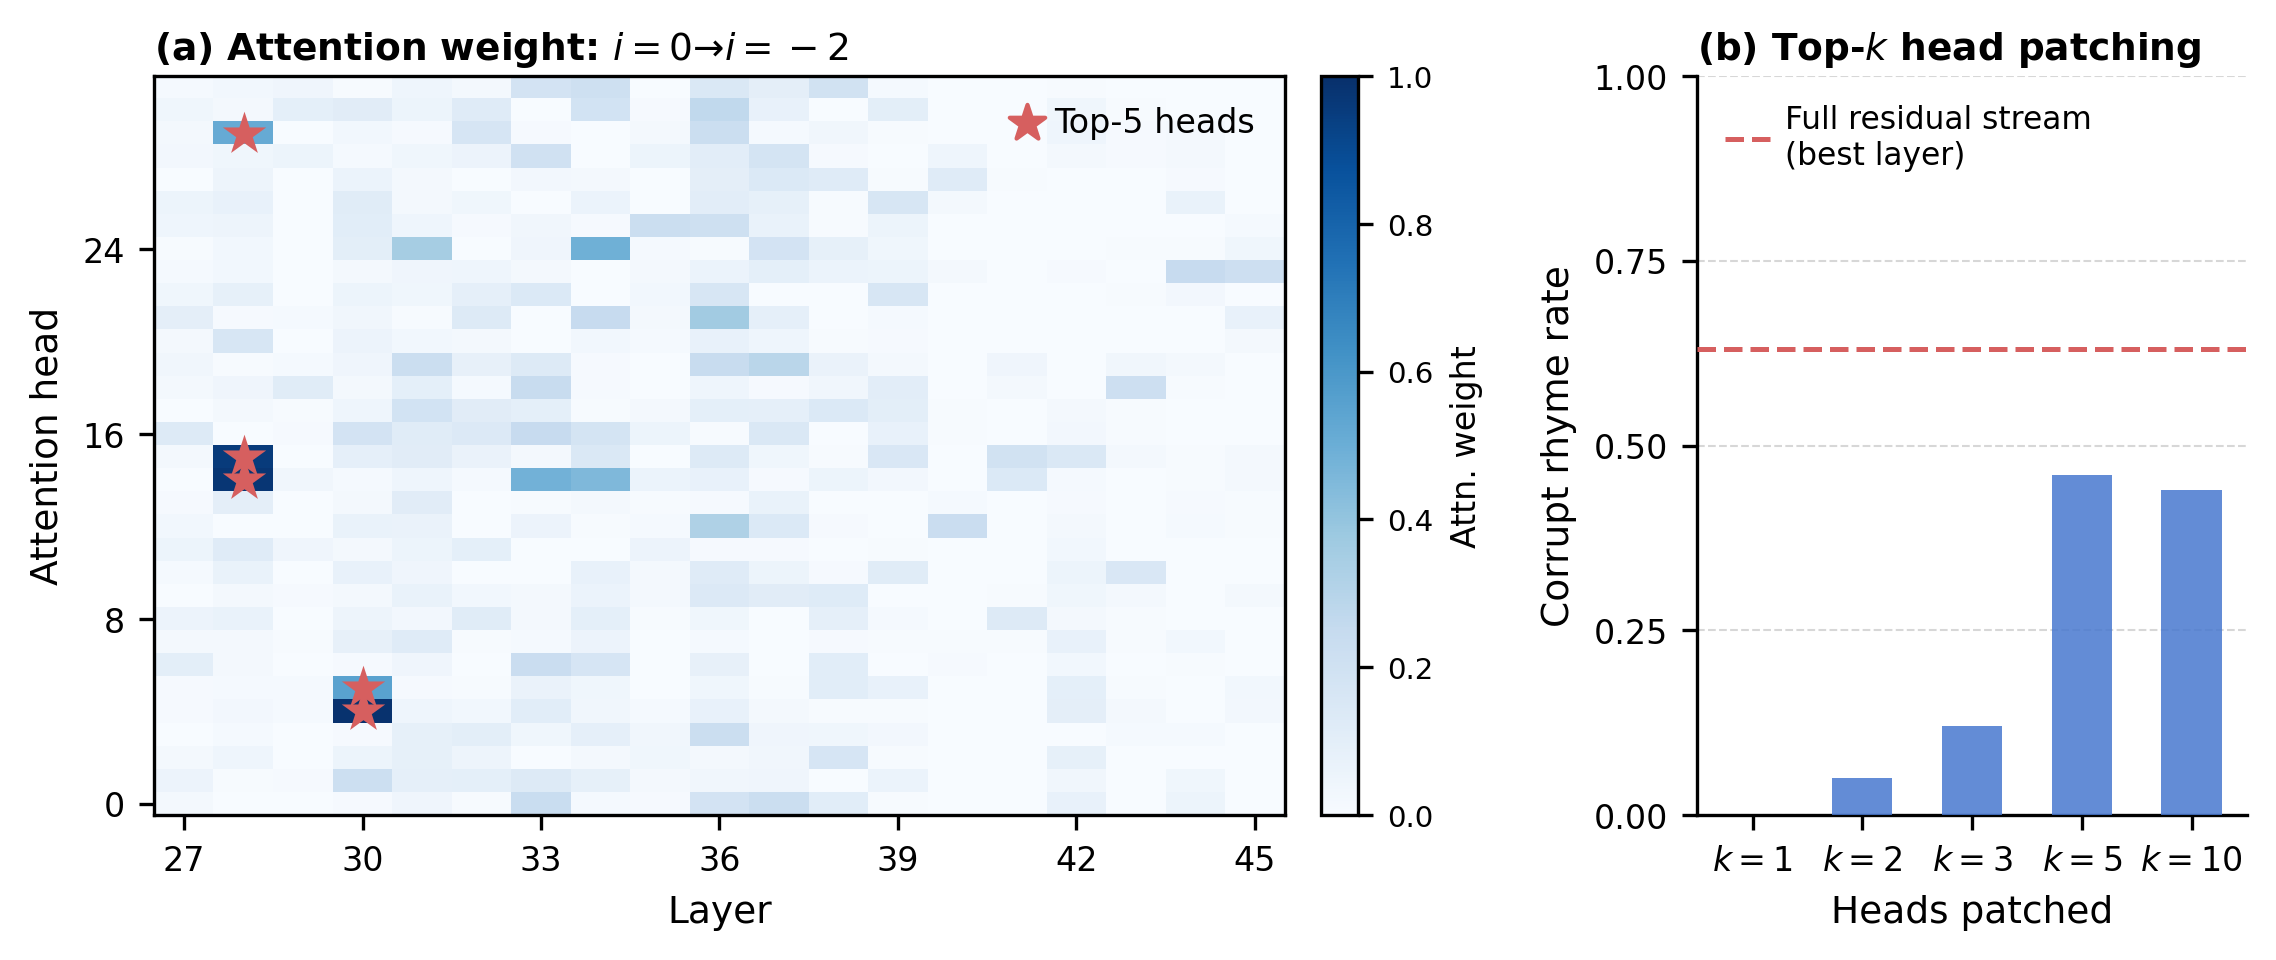
\includegraphics[width=\linewidth]{media/results-patching/topk_head_patching.png}
    \caption{Localizing the planning site handoff in Gemma-3-27B to a sparse set of attention heads. \textbf{(a)} Attention weight from the newline token ($i=0$) to the last word token ($i=-2$) across heads in layers 27--45. Red stars mark the top-5 heads by attention weight. \textbf{(b)} Corrupt rhyme rate when patching the top-$k$ highest-attending heads simultaneously at the newline. The dashed line shows the reference level from full residual-stream patching at the best single layer (${\sim}0.63$).}
    \label{fig:topk-heads}
\end{figure}

% We apply activation patching at the last word token (position $-1$ in Qwen3, $-2$ in
% Gemma-3 and Llama; see Appendix~\ref{sec:model-config}) and at the newline ($i=0$)
% across all layers. Clean and corrupted prompts differ only in the last word of the first
% line, inducing different target rhyme families (e.g., \textit{fright} versus
% \textit{fear}). We report the corrupt rhyme rate averaged over 5 prompt pairs (100
% samples per layer per position). Appendix~\ref{sec:patching-baselines} provides
% zero-vector and donor-prompt controls confirming all effects are causally specific.
% The last word is the positive control: it always carries the rhyme word's identity.
% The newline is the candidate planning site. The information routing handoff is the key
% diagnostic: if the causal locus migrates from the last word to the newline, last-word
% patching effectiveness should drop and newline effectiveness should rise simultaneously.

% \subsection{Last Word Token: Positive Control}
% \label{sec:patch-lastword}

% \begin{figure}[h]
% \centering
% \fbox{\parbox{0.85\textwidth}{\centering\vspace{2cm}
% \textbf{[PLACEHOLDER: Last word patching across all models and scales.
% One representative model per family shown (e.g., Gemma-3-27B, Qwen3-32B, Llama-70B),
% with additional smaller models shown as lighter lines. Y-axis: corrupt rhyme rate
% (0 to 1). X-axis: layer index. All models should show uniformly high corrupt rhyme rate
% ($\sim$0.65--0.80) across most layers, confirming the positive control.]}
% \vspace{2cm}}}
% \caption{Corrupt rhyme rate under activation patching at the last word token, across all
% model families and scales. All models show high corrupt rhyme rates across most layers,
% confirming that the rhyme word's identity is causally encoded at this position throughout.
% This is conditioning on a nearby stimulus, not planning site formation.}
% \label{fig:lastword-patching}
% \end{figure}

% Patching at the last word token is highly effective across all layers for all tested
% models (Figure~\ref{fig:lastword-patching}), confirming that the pipeline is effective
% and establishing the reference level against which newline patching is compared. High
% last-word patching is not evidence of planning site formation---it reflects conditioning
% on a nearby stimulus.

% \subsection{Newline Token: Planning Site Detection}
% \label{sec:patch-newline}

% \begin{figure}[h]
% \centering
% \fbox{\parbox{0.85\textwidth}{\centering\vspace{2cm}
% \textbf{[PLACEHOLDER: Newline patching across all models and scales.
% Organized by model family. Three panels: (1) Gemma-3 family at all sizes (1B, 4B, 12B,
% 27B) --- Gemma-3-27B should show a clear peak in layers 33--35 ($\sim$0.63); smaller
% models should show near-zero. (2) Qwen3 family at all sizes (0.6B through 32B) --- all
% sizes should show near-zero across all layers. (3) Llama family (1B, 3B, 8B, 70B) ---
% all sizes near-zero across all layers. Use the same y-axis (0 to 1) across all panels.]}
% \vspace{2cm}}}
% \caption{Corrupt rhyme rate under activation patching at the newline token ($i=0$)
% across all model families and scales. Gemma-3-27B is the sole model showing substantial
% causal effect (peak ${\sim}0.63$ in layers 33--35). All other models --- all Qwen3 sizes,
% smaller Gemma-3 models, all Llama models --- show near-zero corrupt rhyme rates. The
% probe signal continuum from Section~\ref{sec:probe-couplets} does not correspond to a
% continuum in causal deployment.}
% \label{fig:newline-patching}
% \end{figure}

% Figure~\ref{fig:newline-patching} shows the layer-wise newline patching results.
% Gemma-3-27B is the sole model showing substantial causal effect, peaking at ${\sim}0.63$
% in layers 33--35. Every other model shows near-zero causal effect:

% \textit{Qwen3 at all scales.} Despite consistent planning-compatible representations at
% the newline (Figure~\ref{fig:poem-results}), all Qwen3 models from 0.6B to 32B
% show near-zero corrupt rhyme rates when patched at the newline. This within-family
% result is the paper's most important methodological finding: Qwen3 forms
% planning-compatible representations at the newline without those representations being
% causally active during generation. The probe signal and patching result are dissociable.

% \textit{Smaller Gemma-3 models.} Gemma-3 models below 27B show near-zero causal effect.
% The information routing handoff is specific to the 27B scale, not a general property of
% the Gemma-3 architecture.

% \textit{Llama at all scales.} Llama models from 1B to 70B show near-zero newline
% patching, consistent with minimal probe signal.

% All-layer patching at the newline (Appendix~\ref{sec:patch-all-layers}) confirms these
% results: patching all layers simultaneously at $i=0$ produces 73\% corrupt rhyme rate
% in Gemma-3-27B, 9\% in Qwen3-32B, and approximately \textbf{[FILL]}\% in Llama-70B.
% The ordering matches the categorical distinction from single-layer patching.

% \subsection{The Information Routing Handoff in Gemma-3-27B}
% \label{sec:handoff}

% \begin{figure}[H]
%     \centering
%     \begin{subfigure}{\linewidth}
%         \centering
%         \subcaption[]{Qwen3-32B: no handoff.}
%         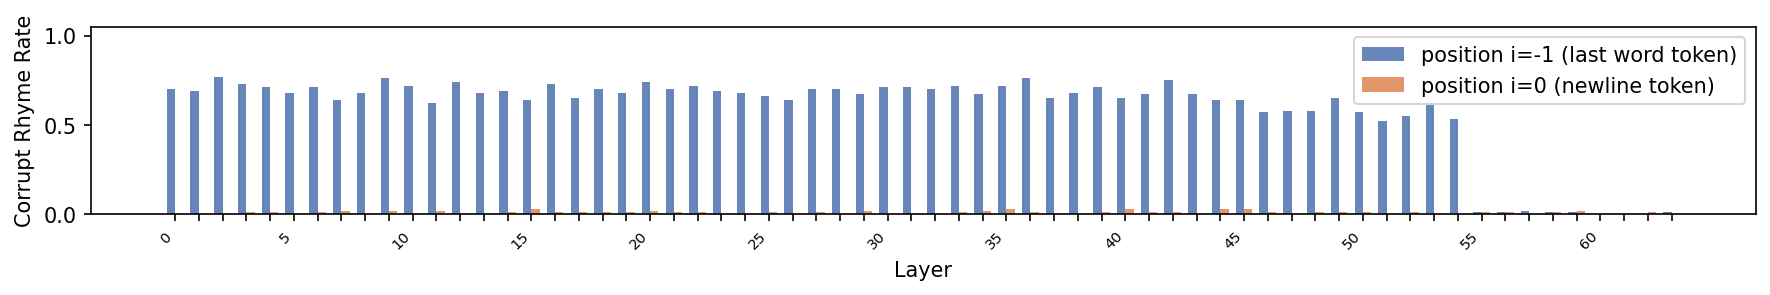
\includegraphics[width=\linewidth]{media/results-patching/qwen3_32b_aggregate.png}
%     \end{subfigure}
%     \hfill
%     \begin{subfigure}{\linewidth}
%         \centering
%         \subcaption[]{Gemma-3-27B: information routing handoff.}
%         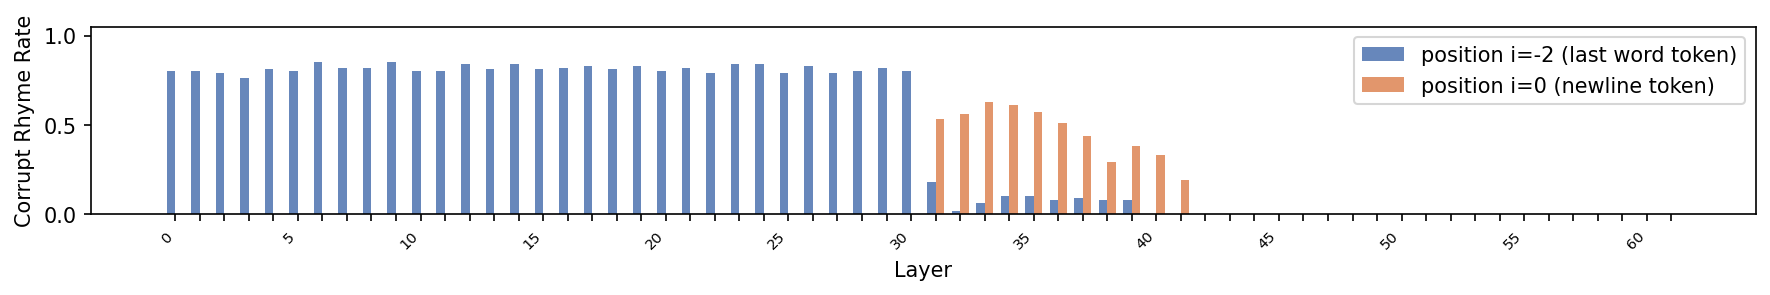
\includegraphics[width=\linewidth]{media/results-patching/gemma3_27b_aggregate.png}
%     \end{subfigure}
%     \caption{Corrupt rhyme rates at the last word and newline positions across all layers,
%     averaged over 5 prompt pairs (100 samples per layer). In Gemma-3-27B, last-word
%     patching drops sharply around layer 30 while newline patching rises simultaneously ---
%     the information routing handoff. In Qwen3-32B, last-word patching remains high and
%     newline patching near zero throughout. All tested Llama models and smaller Gemma-3
%     models mirror the Qwen3 pattern.}
%     \label{fig:patch-results}
% \end{figure}

% Figure~\ref{fig:patch-results} shows the layer-wise comparison in Qwen3-32B and
% Gemma-3-27B. In Gemma-3-27B, last-word patching is highly effective in early layers
% (corrupt rhyme rate ${\sim}0.80$, layers 0--29). Around layer 30, last-word effectiveness
% drops sharply while newline patching rises from near zero to ${\sim}0.63$, peaking at
% layers 33--35. The causal locus has migrated from the word token to the newline.

% This transition is the mechanistic signature of planning site formation. Gemma-3-27B
% actively migrates the causal locus rather than passively accumulating rhyme information.
% By layer 30, the word token's direct causal influence has been abstracted away, and the
% newline residual stream has become the primary read-out site for the phonological
% constraint---separating the representation of \textit{what the rhyme word is} (carried
% at the last word in early layers) from \textit{what phonological family is required}
% (written to the newline in later layers).

% In Qwen3-32B, no such transition occurs: last-word patching remains uniformly high
% (${\sim}0.65$--$0.77$) across all 64 layers; newline patching remains near zero.
% All other tested models---all Qwen3 sizes, smaller Gemma-3 models, all Llama
% models---mirror this pattern.

% Full results across all six swept token positions are in
% Appendix~\ref{sec:additional-patching-details} (Figure~\ref{fig:patching-all-positions}).
% The comma token at position $i=-1$ in Gemma-3-27B shows near-zero causal effect
% throughout, confirming the handoff is specific to the newline token.

% \subsection{Attention Head Patching: Localizing the Planning Site}
% \label{sec:head-patching}

% We patch individual attention head outputs at the newline position within Gemma-3-27B's
% planning layer range (30--40) and compare against full residual stream patching.

% \begin{figure}[h]
% \centering
% \fbox{\parbox{0.85\textwidth}{\centering\vspace{2cm}
% \textbf{[PLACEHOLDER: Attention head patching at Gemma-3-27B's planning layers.
% Heatmap or bar chart showing, for each attention head in layers 30--40 of Gemma-3-27B,
% the corrupt rhyme rate under patching that head's output at $i=0$. Show the full
% residual stream patching corrupt rhyme rate as a reference line ($\sim$0.63).
% Expected result: no individual head approaches the full residual stream patching level,
% indicating the planning representation is distributed.]}
% \vspace{2cm}}}
% \caption{Per-head patching at the newline position in Gemma-3-27B's planning layers
% (30--40). Individual attention heads produce substantially lower corrupt rhyme rates
% than full residual stream patching, indicating the planning representation is distributed
% across multiple components. Path patching is the natural next step.}
% \label{fig:head-patching}
% \end{figure}

% Individual head patching produces substantially lower corrupt rhyme rates than full
% residual stream patching (Figure~\ref{fig:head-patching}). The planning representation
% is not localized in a single head but distributed across the residual stream. This
% refines the finding: the newline residual stream in layers 30--40 is the causal locus,
% but the mechanism \textit{writing} to it is distributed. Path patching~\citep{wang2022ioi}
% is the appropriate next step.

% \subsection{Steering Vectors: Independent Corroboration}
% \label{sec:steering}

% We compute steering vectors $\mathbf{v}_{\ell,i} = \text{mean}(\mathbf{h}_{\ell,i}^{(r)})
% - \text{mean}(\mathbf{h}_{\ell,i}^{(c)})$ from 100 clean and 100 corrupted prompts per
% rhyme family, and add $\alpha \mathbf{v}_{\ell,i}$ at a single position and layer during
% generation, following~\cite{maar2026whatsplanmetricsimplicit} with $\alpha=1.5$.

% \begin{figure}[h]
%     \centering
%     \begin{subfigure}{\linewidth}
%         \centering
%         \subcaption[]{Steering Effectiveness in Qwen3-32B.}
%         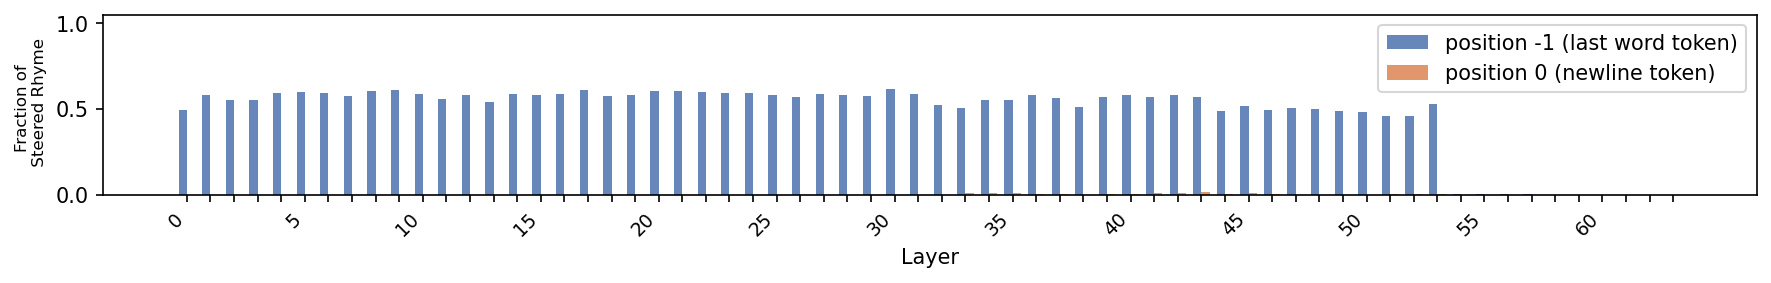
\includegraphics[width=\linewidth]{media/results-steer/qwen-steer.png}
%     \end{subfigure}
%     \hfill
%     \begin{subfigure}{\linewidth}
%         \centering
%         \subcaption[]{Steering Effectiveness in Gemma-3-27B.}
%         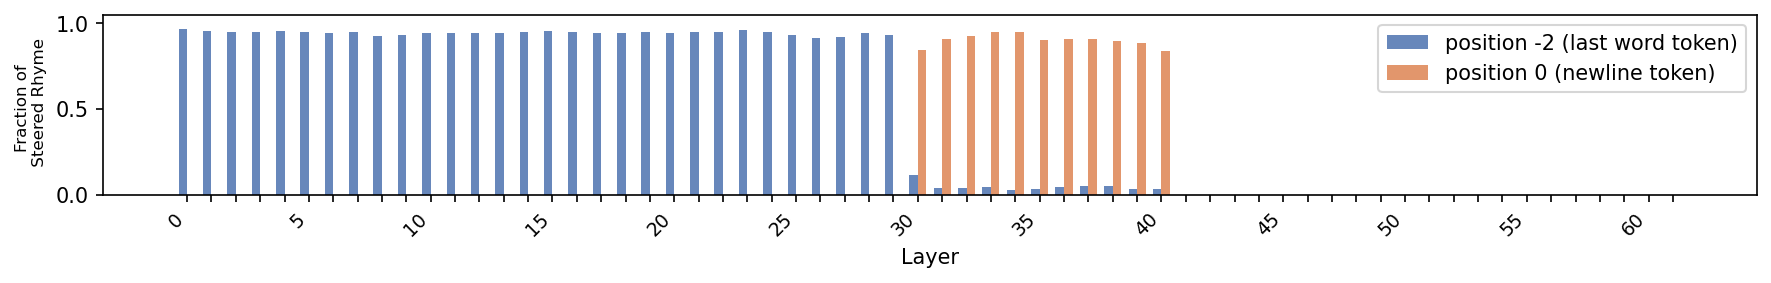
\includegraphics[width=\linewidth]{media/results-steer/gemma-steer.png}
%     \end{subfigure}
%     \caption{Steering effectiveness at the last word and newline positions. In
%     Gemma-3-27B, newline steering is effective in layers 30--40, corroborating the
%     patching evidence for a causally active planning site in exactly the same layer range.
%     In Qwen3-32B, newline steering produces little effect, consistent with near-zero
%     patching. The two methods converge.}
%     \label{fig:steer-results}
% \end{figure}

% \begin{figure}[h]
% \centering
% \fbox{\parbox{0.85\textwidth}{\centering\vspace{2cm}
% \textbf{[PLACEHOLDER: Newline steering effectiveness across all models.
% Organized by model family, same structure as Figure~\ref{fig:newline-patching}. Three
% panels: (1) Gemma-3 family: Gemma-3-27B shows clear effectiveness in layers 30--40;
% smaller models show near-zero. (2) Qwen3 family: all sizes show near-zero or weak
% effect. (3) Llama family: near-zero across all sizes. Same y-axis across all panels.]}
% \vspace{2cm}}}
% \caption{Steering effectiveness at the newline across all model families and scales.
% The pattern mirrors patching: Gemma-3-27B is the sole model showing clear effectiveness
% (layers 30--40); all other models show near-zero or weak effect.}
% \label{fig:steer-all-models}
% \end{figure}

% Newline steering results (Figures~\ref{fig:steer-results} and~\ref{fig:steer-all-models})
% corroborate the patching findings: Gemma-3-27B shows effective newline steering in
% layers 30--40, coinciding precisely with the patching peak; all other tested models
% show near-zero newline steering effect.

% Maar et al.'s~\cite{maar2026whatsplanmetricsimplicit} steering sweep provides independent
% cross-paper corroboration. In their Figure 26, Gemma-3-27B and Gemma-2-27B are dramatic
% outliers in newline steering effectiveness---the rest of the models cluster near zero.
% This convergent finding from a different group and experimental setup provides strong
% evidence that the outlier status is a robust property of the model, not an artifact of
% our methodology. Critically, this reconciles with Maar et al.'s broader result: their
% last-word steering is highly effective across all models (consistent with our positive
% control), while only Gemma-3-27B and Gemma-2-27B stand out specifically at the newline.


% \section{Analysis}
% \label{sec:analysis}

% \subsection{Planning Site Formation: Where and When It Occurs}
% \label{sec:analysis-formation}

% \begin{figure}[h]
% \centering
% \fbox{\parbox{0.85\textwidth}{\centering\vspace{2cm}
% \textbf{[PLACEHOLDER: Peak newline patching effectiveness vs.\ model size.
% Line plot with x-axis = model size (parameters, log scale) and y-axis = peak single-layer
% corrupt rhyme rate at the newline position (maximum over all layers). Three lines:
% Gemma-3 (near-zero for 1B, 4B, 12B; substantial at 27B $\sim$0.63), Qwen3 (near-zero
% across all sizes from 0.6B to 32B), Llama (near-zero from 1B to 70B). A dashed
% horizontal line marks the last-word patching level ($\sim$0.70--0.80).]}
% \vspace{2cm}}}
% \caption{Peak corrupt rhyme rate at the newline under single-layer patching as a
% function of model size. Gemma-3-27B is a clear outlier. All Qwen3 and Llama sizes
% remain near zero regardless of scale, demonstrating the routing handoff is not a
% function of model size but is specific to Gemma-3-27B.}
% \label{fig:patching-scaling}
% \end{figure}

% Figure~\ref{fig:patching-scaling} synthesizes patching results across all models.
% The information routing handoff is unique to Gemma-3-27B: not a general property of
% large models (Qwen3-32B and Llama-70B show near-zero newline patching), not a general
% Gemma-3 property (models below 27B show near-zero), and not a simple scaling effect
% within the Gemma-3 family. The independent corroboration from Maar et al.\ rules out a
% methodological artifact---if the handoff were one, it would not appear in their
% independent steering sweep.

% \subsection{The Encoding/Deployment Dissociation}
% \label{sec:analysis-dissociation}

% The Qwen3 within-family result provides the sharpest evidence for the dissociation
% between planning-compatible representations and causally active planning sites. At every
% tested Qwen3 scale---0.6B to 32B---probing reveals elevated $i=0$ probe signal, yet
% patching produces near-zero corrupt rhyme rates. This replicates the dissociation across
% multiple model checkpoints within a single family under controlled conditions where
% training objective, tokenization, and architecture are held constant.

% This has direct methodological implications. Prior steering-based
% work~\citep{maar2026whatsplanmetricsimplicit} identifies planning signals across many
% model families. Our results clarify why: last-word positions always carry
% rhyme-compatible representations (confirmed by our positive control), making last-word
% steering effective everywhere. What patching adds is the ability to distinguish models
% where the newline is a causally active planning site from those where it merely carries
% a planning-compatible representation.

% \subsection{What the Handoff Reveals About Planning Site Construction}
% \label{sec:analysis-handoff}

% The routing handoff reveals a two-stage computation in Gemma-3-27B. In early layers
% (0--29), causal information is concentrated at the word token, represented as word
% identity. In later layers (30--40), it has moved to the newline: the newline residual
% stream carries the phonological constraint while the word token's direct causal influence
% has been reduced. Rhyme planning information has been abstracted from specific word
% identity to phonological family and written to a dedicated position before generation
% begins.

% This two-stage structure separates planning from execution: the phonological plan is
% formed at the newline and read out during second-line generation, rather than requiring
% the model to attend back to the first-line word token at each step. Whether this
% emerges from specific properties of Gemma-3-27B's training or architecture is an open
% question; the presence of the handoff in Gemma-2-27B (per Maar et al.'s steering
% results) suggests it may persist across Gemma generations at the 27B scale.


\section{Conclusion}

We introduced the notion of \textit{planning site formation} and investigated it across three model families and more than ten model sizes using linear probing and activation patching. Our central finding is a categorical dissociation: Gemma-3-27B is the only model that forms a causally active planning site at the newline token, doing so via an information routing handoff in which the causal locus migrates from the last word token to the newline around layer 30. Every other tested model---all Qwen3 sizes from 0.6B to 32B, all Llama-3 sizes from 1B to 8B, and all smaller Gemma-3 models---conditions on the last word token throughout generation.

The Qwen3 family provides the paper's sharpest methodological lesson. Probing reveals strong, scale-dependent planning-compatible representations at the newline across all Qwen3 sizes, yet activation patching shows near-zero causal effect at every scale. Planning-compatible representations and causally active planning sites are dissociable: probe signal is not sufficient evidence of a planning site, and activation patching is required to establish causal relevance.

Beyond the layer-level analysis, we localize the handoff in Gemma-3-27B to a sparse set of five attention heads in layers 28--34, identified via attention weight ranking followed by simultaneous head patching. Patching these five heads at the newline recovers ${\sim}73\%$ of the effect achievable by full residual-stream patching, while single-head patching and MLP patching produce no effect. This circuit-level specificity---a handful of attention heads implementing a representational handoff---suggests that planning site formation, when it occurs, is a structured computational phenomenon rather than a diffuse property of many model components.

Our probe-then-patch methodology requires no transcoder training and far less data than steering vector approaches, making it scalable to large models across many architectures. The results, however, also surface important open questions and limitations that future work should address.

First, our analysis is limited to three model families on a single structured generation task (rhyming couplets). The categorical distinction between last-word conditioning and planning site formation may be specific to this task, this architecture, or this scale regime. Extending the methodology to prose generation, code completion, and multi-step reasoning tasks would test whether the representational handoff is a general planning primitive or a narrow phonological phenomenon. Second, while we localize the Gemma-3-27B handoff to five attention heads, we do not yet trace the full information-flow circuit. Path patching~\citep{goldowsky2023localizing} from the last word token through these heads to the downstream generation would clarify whether the circuit is feedforward or involves recursive refinement. Third, the absence of the handoff in all Qwen3 and Llama-3 models despite strong probe signal raises a question about what distinguishes Gemma-3-27B: is it an architectural feature (e.g.\ differences in attention masking or layer normalization), a training data property, or a scale threshold within the Gemma family that is not reached by the 12B model? Probing and patching Gemma-3-27B against Gemma-3-12B directly would isolate the scale effect. Finally, our baselines confirm the causal specificity of the patching signal, but leave open whether the planning representation at the newline is \textit{read} by the model during generation or whether it exerts influence only when artificially inserted via patching. Causal scrubbing~\citep{chan2022causal} or activation steering experiments targeting the planning heads would help distinguish these possibilities.


\bibliography{references}
\bibliographystyle{colm2026_conference}

\appendix

\section{Model Configurations}
\label{sec:model-config}
For reference, we report details of the architectural differences between models. 

\begin{table}[h]
\centering
\begin{tabular}{lccc}
\toprule
 & Qwen3-32B & Gemma-3-27B  & Llama-3.1-8B \\
\midrule
vocabulary size, $|\mathcal V|$ & 151,936 & 262,208 & 128,256 \\
hidden dimension, $d$           & 5,120   & 5,376   & 4,096  \\
number of layers, $L$           & 64      & 62      & 32     \\
\bottomrule
\end{tabular}
\label{tab:models}
\end{table}

We also note important tokenization differences. Qwen and Llama treat \texttt{,\textbackslash n} as a single token, while Gemma treats
\texttt{,} and \texttt{\textbackslash n} as separate tokens. 
This places the last word $r_1$ at position $-1$ in Qwen and Llama and position $-2$ in Gemma.

\begin{table}[h]
\centering
\begin{tabular}{cccccccccc}
\toprule
Position: & $\dots$ & $-3$ & $-2$ & $-1$ & $0$ & $1$ & $2$ & $3$ & $\dots$ \\
\midrule
Qwen3:   & $\dots$ & $\texttt{of}$ & $\texttt{of}$    & $\texttt{fright}$ & \texttt{,\textbackslash n} & \texttt{and} & \texttt{hoped} & \texttt{that} & $\dots$ \\
Llama-3: & $\dots$ & $\texttt{of}$ & $\texttt{of}$    & $\texttt{fright}$ & \texttt{,\textbackslash n} & \texttt{and} & \texttt{hoped} & \texttt{that} & $\dots$\\
Gemma-3: & $\dots$ & $\texttt{of}$ & $\texttt{fright}$ & $\texttt{,}$      & \texttt{\textbackslash n}  & \texttt{and} & \texttt{hoped} & \texttt{that} & $\dots$ \\
\bottomrule
\end{tabular}
\end{table}


\section{Additional Probing Results}
\label{sec:additional-probing-results}
For probing experiments, we also evaluated on top-1 accuracy. Note these are similar to the reported results, only scaled down. 

\begin{figure}[H]
    \centering
    \begin{subfigure}{0.325\linewidth}
        \centering
        \subcaption[]{Qwen3-32B.}
        
\includegraphics[width=\linewidth]{media/results-probe/qwen-top1.png}
    \end{subfigure}
    \begin{subfigure}{0.325\linewidth}
        \centering
        \subcaption[]{Gemma-3-27B.}
        
\includegraphics[width=\linewidth]{media/results-probe/gemma-top1.png}
    \end{subfigure}
    \begin{subfigure}{0.325\linewidth}
        \centering
        \subcaption[]{Llama-3.1-80B}
        
\includegraphics[width=\linewidth]{media/results-probe/gemma-top1.png}
    \end{subfigure}
    \caption{Top-1 probe accuracy on general text. Mirrors top-5 results.}
    \label{fig:appendix-probe}
\end{figure}

\begin{figure}[H]
    \centering
    \begin{subfigure}{0.325\linewidth}
        \centering
        \subcaption[]{Qwen3-32B}
        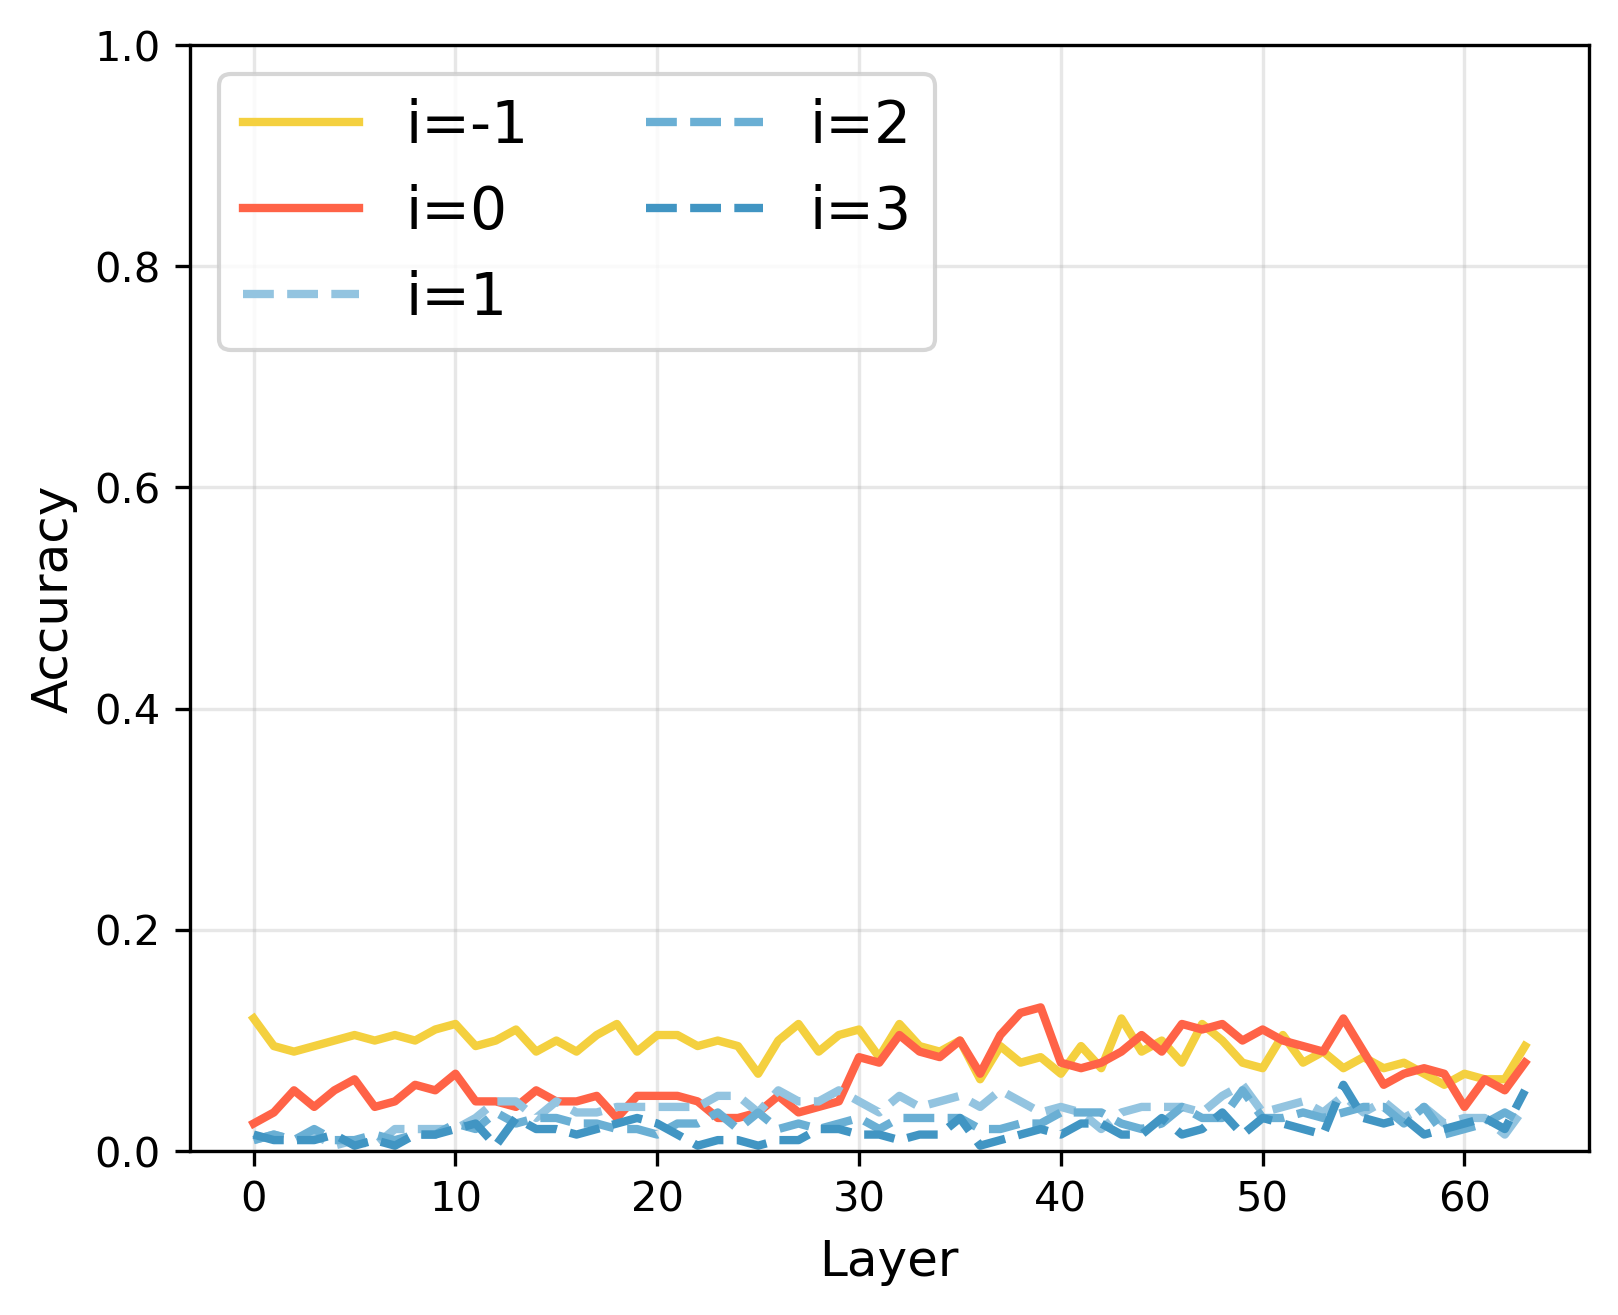
\includegraphics[width=\linewidth]{media/results-poem/qwen-top1.png}
    \end{subfigure}
    \hfill
    \begin{subfigure}{0.325\linewidth}
        \centering
        \subcaption[]{Gemma-3-27B}
        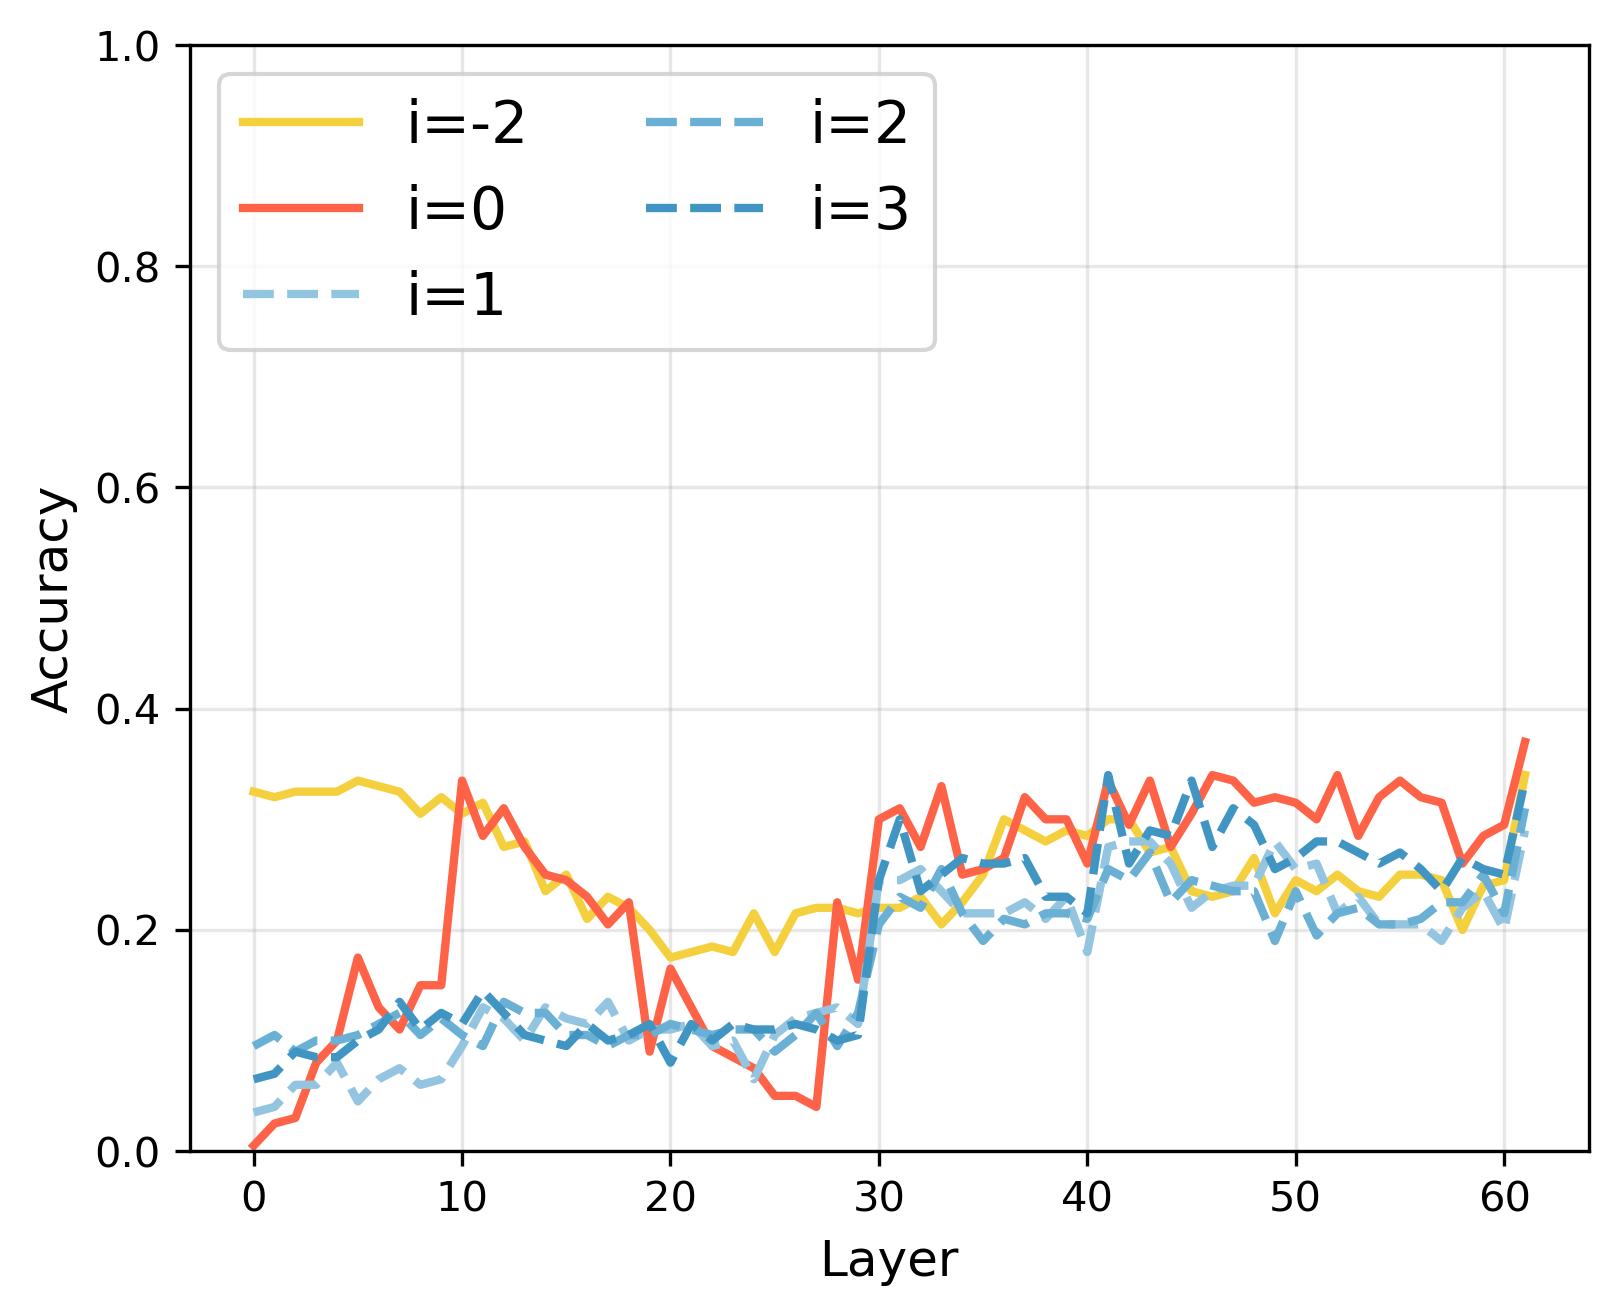
\includegraphics[width=\linewidth]{media/results-poem/gemma-top1.png}
    \end{subfigure}
    \begin{subfigure}{0.325\linewidth}
        \centering
        \subcaption[]{Llama-3.1-80B}
        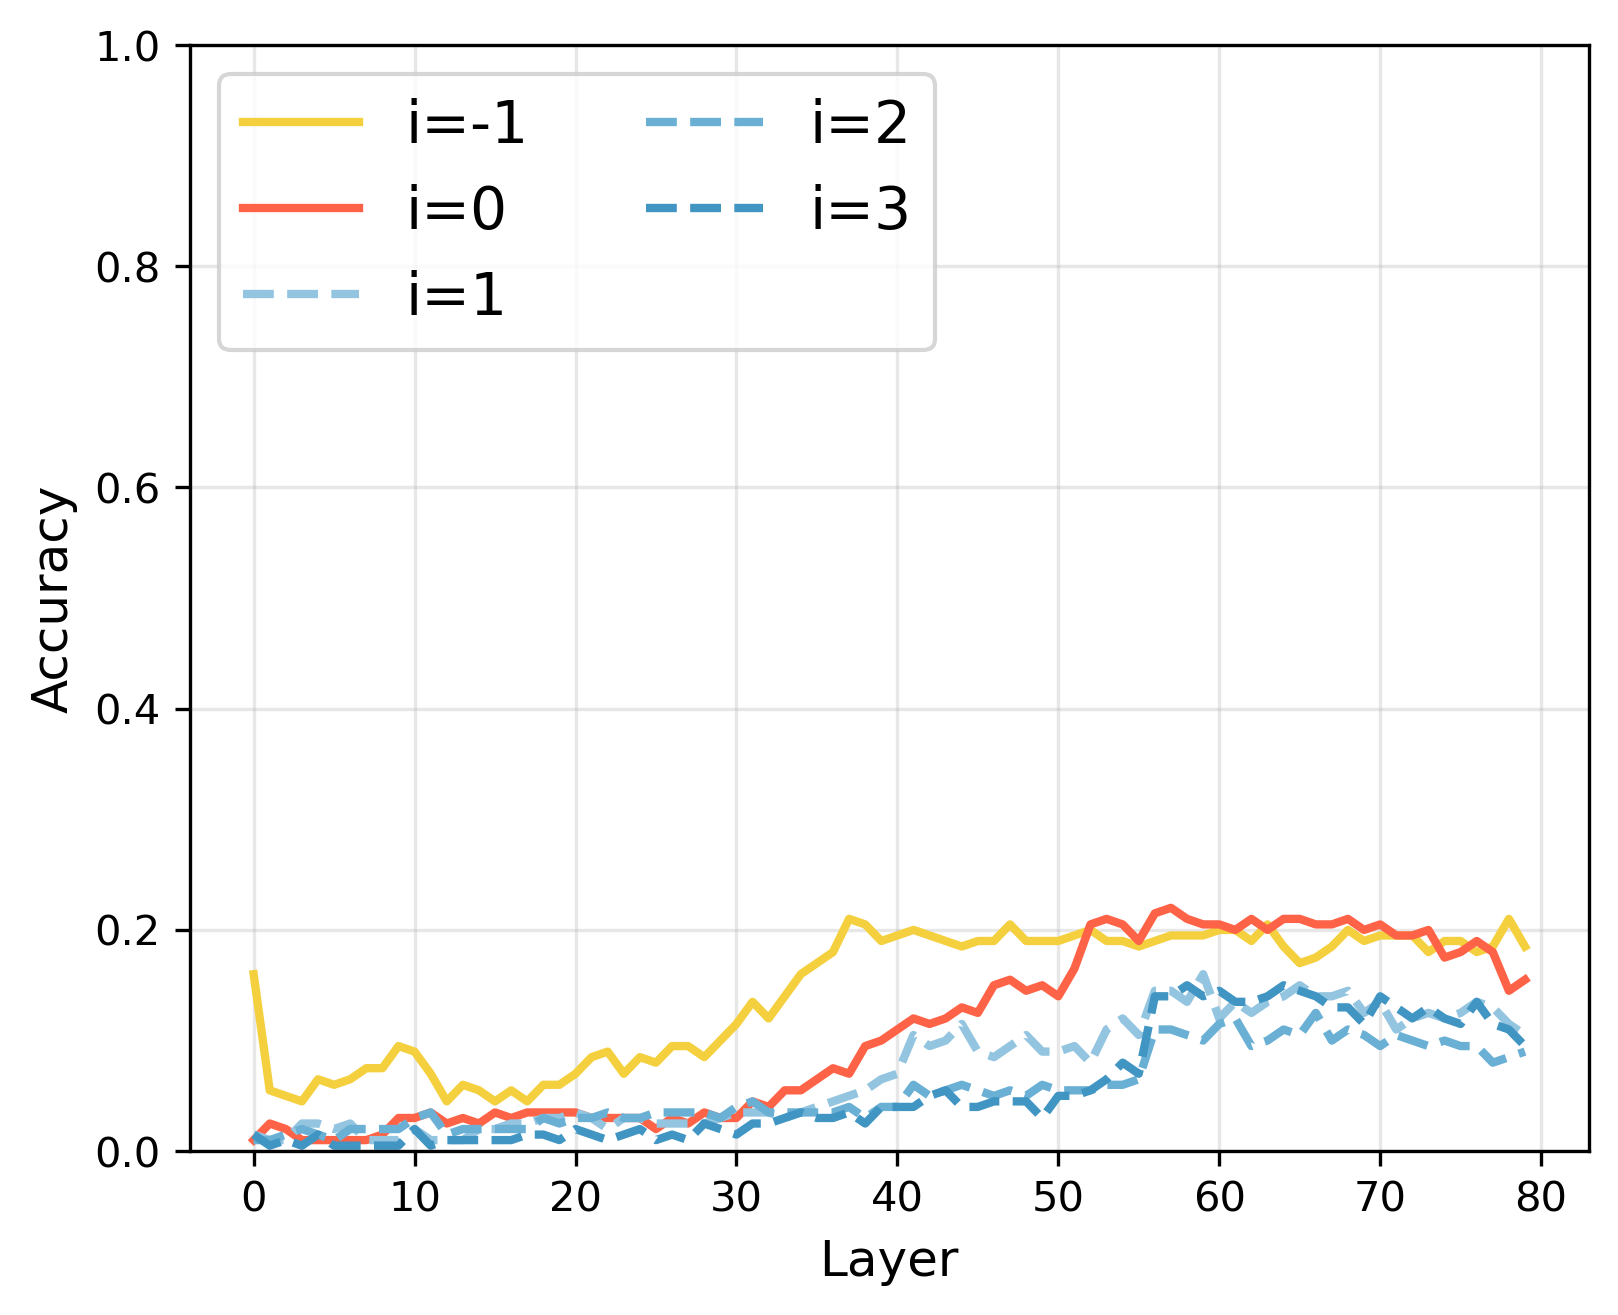
\includegraphics[width=\linewidth]{media/results-poem/llama-top1.png}
    \end{subfigure}

    \caption{Top-1 probe accuracy on general text. Mirrors top-5 and rhyme accuracy results.}
    \label{fig:appendix-poem}
\end{figure}


\section{Additional Activation Patching Details}
\label{sec:additional-patching-details}

\subsection*{Baselines}
\label{sec:patching-baselines}

To verify that the observed corrupt rhyme rates reflect the specific encoding of the corrupt rhyme word rather than a generic effect of perturbing the residual stream, we run two control conditions. The \textit{zero-vector} baseline replaces the patched hidden state with an all-zeros vector, testing whether simply zeroing out that position is sufficient to induce corrupt rhyming. The \textit{donor-prompt} baseline replaces it with a hidden state cached from the same token position in a semantically unrelated sentence (``The weather outside is warm and sunny today, and the birds are singing.''), testing whether any arbitrary non-zero activation can produce the effect.

Figure~\ref{fig:patching-baselines} shows results for Qwen3-32B (at $i=-1$) and Gemma-3-27B (at $i=-2$), averaged over all prompt pairs. Both control conditions produce corrupt rhyme rates near zero across all layers, while true activation patching reaches ${\sim}0.80$ for Gemma-3-27B and ${\sim}0.70$ for Qwen3-32B at their peak layers. This confirms that the effect is causally specific to the identity of the corrupt rhyme word encoded in the residual stream, and not an artifact of activation disruption per se.

\begin{figure}[H]
    \centering
    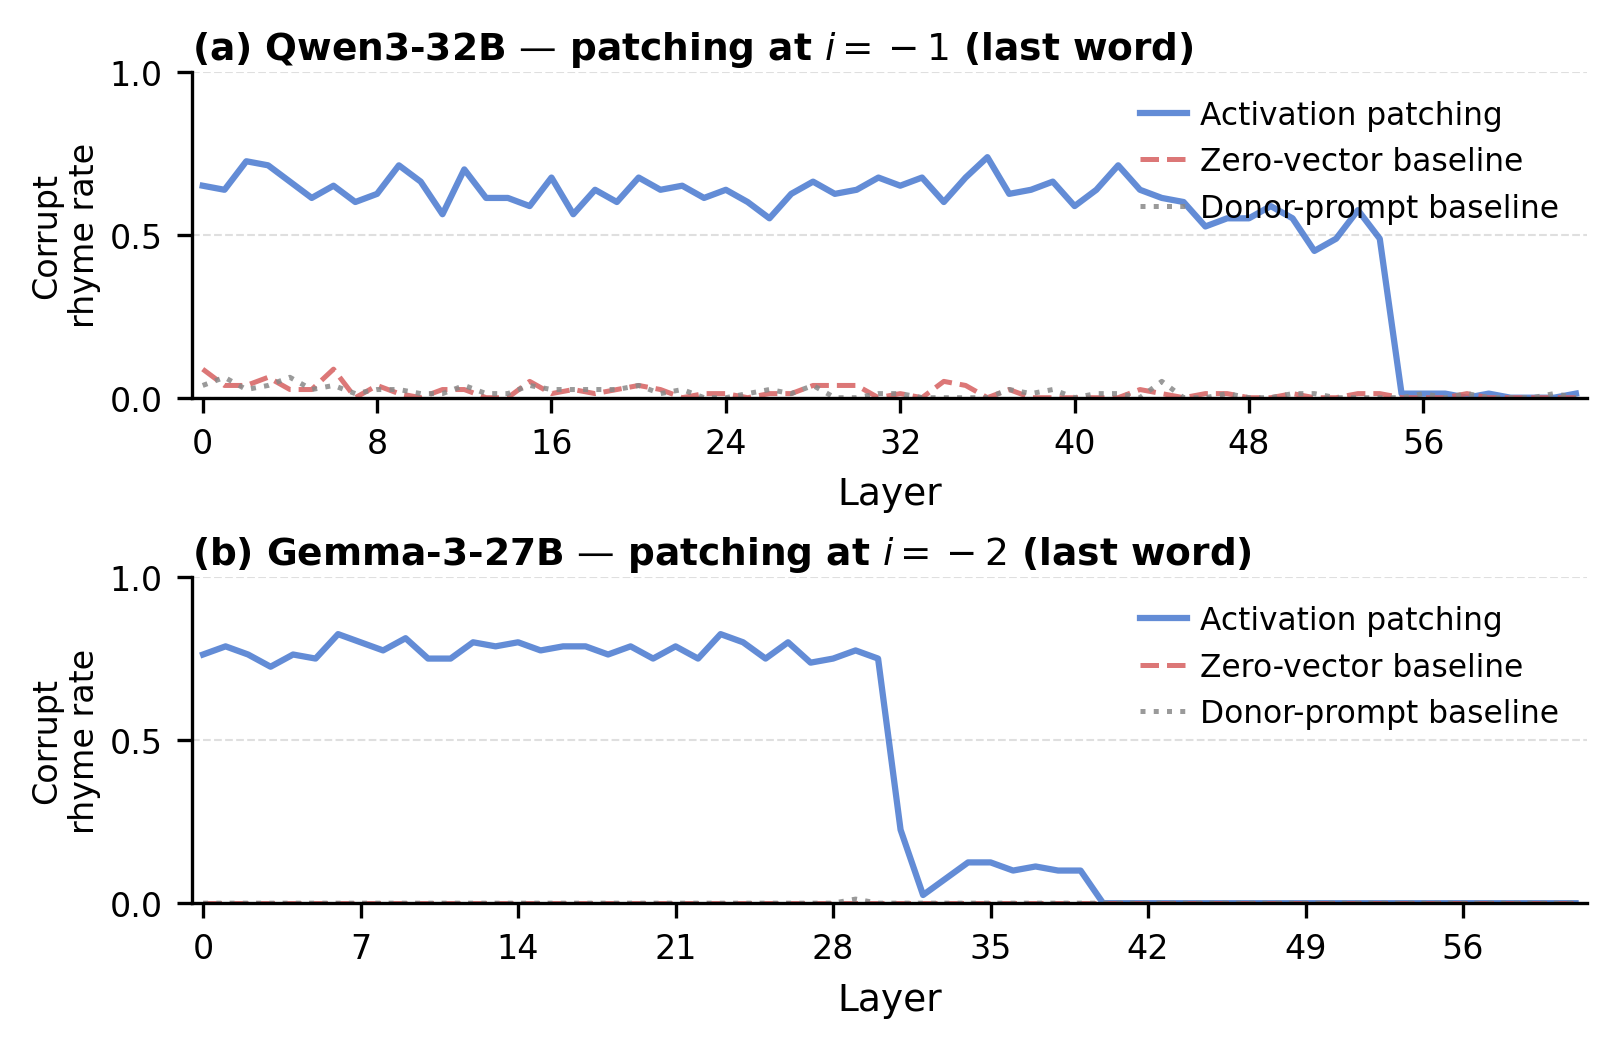
\includegraphics[width=\linewidth]{media/results-patching/patching_baselines.png}
    \caption{Corrupt rhyme rate for true activation patching versus zero-vector and donor-prompt controls, at the last word token position. Both controls produce near-zero rates across all layers.}
    \label{fig:patching-baselines}
\end{figure}

\subsection*{All-Layers Patching}
\label{sec:patch-all-layers}

Table~\ref{tab:patch-all-layers} reports corrupt rhyme rates when all layers are patched simultaneously at a given token position, providing an upper bound on single-position causal influence. Positions $i \geq 1$ (generated tokens) yield zero corrupt rhyme rate in every model and are omitted. The no-patch baseline is 0\% for all models. The results replicate and extend the per-layer findings: Gemma-3-27B stands out with 73\% corrupt rhyme rate at the newline, while all Qwen3 and Llama-3 models show near-zero $i=0$ effectiveness (0--9\%), confirming the categorical absence of a planning site at the newline across these families.

\begin{table}[h]
\centering
\begin{tabular}{llcc}
\toprule
Family & Model & Last Word & $i=0$ (Newline) \\
\midrule
\multirow{6}{*}{Qwen3}
 & 0.6B  &  1 &  7 \\
 & 1.7B  & 15 &  2 \\
 & 4B    & 42 &  7 \\
 & 8B    & 53 &  2 \\
 & 14B   & 63 &  7 \\
 & 32B   & 96 &  9 \\
\midrule
\multirow{4}{*}{Gemma-3}
 & 1B    & 37 &  1 \\
 & 4B    & 78 &  0 \\
 & 12B   & 90 &  0 \\
 & 27B   & 100 & 73 \\
\midrule
\multirow{3}{*}{Llama-3}
 & 1B    & 59 &  2 \\
 & 3B    & 87 &  0 \\
 & 8B    & 79 &  0 \\
\bottomrule
\end{tabular}
\caption{Corrupt rhyme rate (\%) when all layers are patched simultaneously at the last word token and newline ($i=0$). Positions $i \geq 1$ yield 0\% in all models and are omitted. Gemma-3-27B is the only model with substantial newline patching effectiveness.}
\label{tab:patch-all-layers}
\end{table}

\subsection*{Per-Layer Results: All Models}

Figure~\ref{fig:appendix-patch-summary} reports the peak (maximum across layers) corrupt rhyme rate for the last word token and newline at each model size. The pattern from the main paper holds at every scale: Gemma-3-27B is the only model for which newline patching reaches a substantial level; all Qwen3 and Llama-3 models show near-zero newline effectiveness regardless of size, as do the smaller Gemma-3 models. Figures~\ref{fig:appendix-patch-qwen3-small}--\ref{fig:appendix-patch-llama3} show the full per-layer profiles. Blue bars show the corrupt rhyme rate when patching the last word token; orange bars show the rate when patching the newline ($i=0$). The representational handoff visible in Gemma-3-27B---last-word effectiveness dropping sharply around layer 30 while newline rises---is absent in every other model.

\begin{figure}[H]
    \centering
    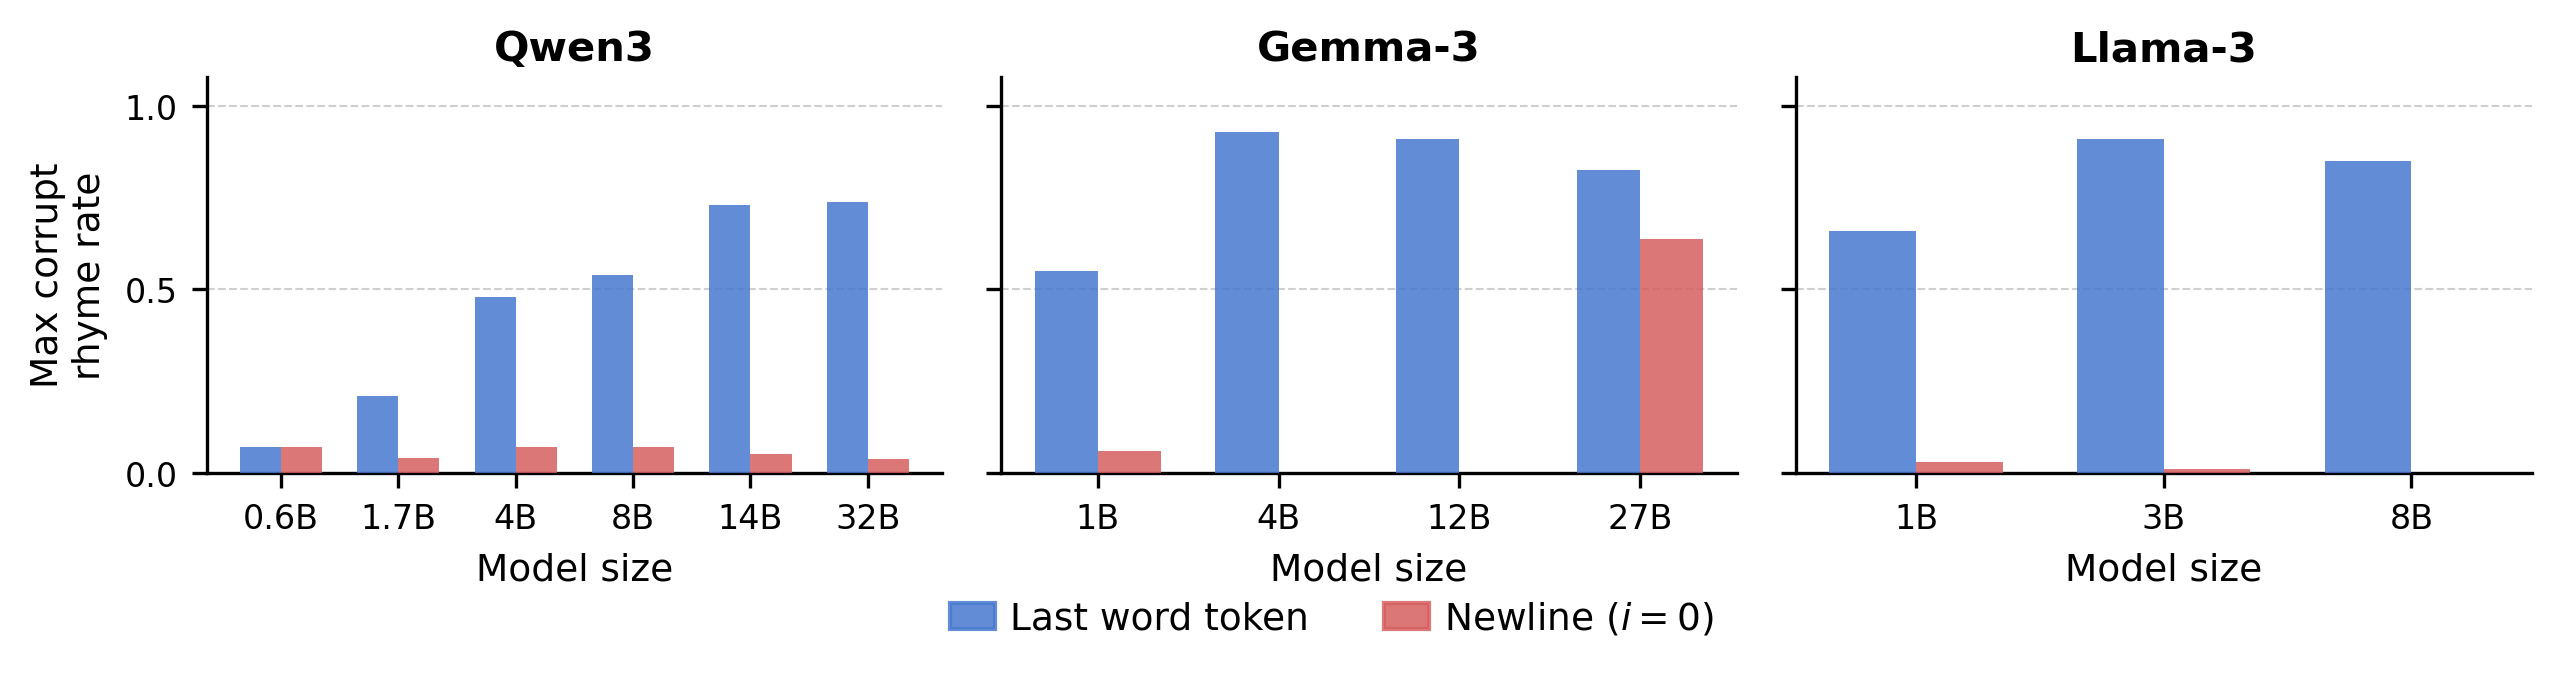
\includegraphics[width=\linewidth]{media/results-patching/patching_summary_bars.png}
    \caption{Peak corrupt rhyme rate (max across layers) per position and model size.}
    \label{fig:appendix-patch-summary}
\end{figure}

\begin{figure}[H]
    \centering
    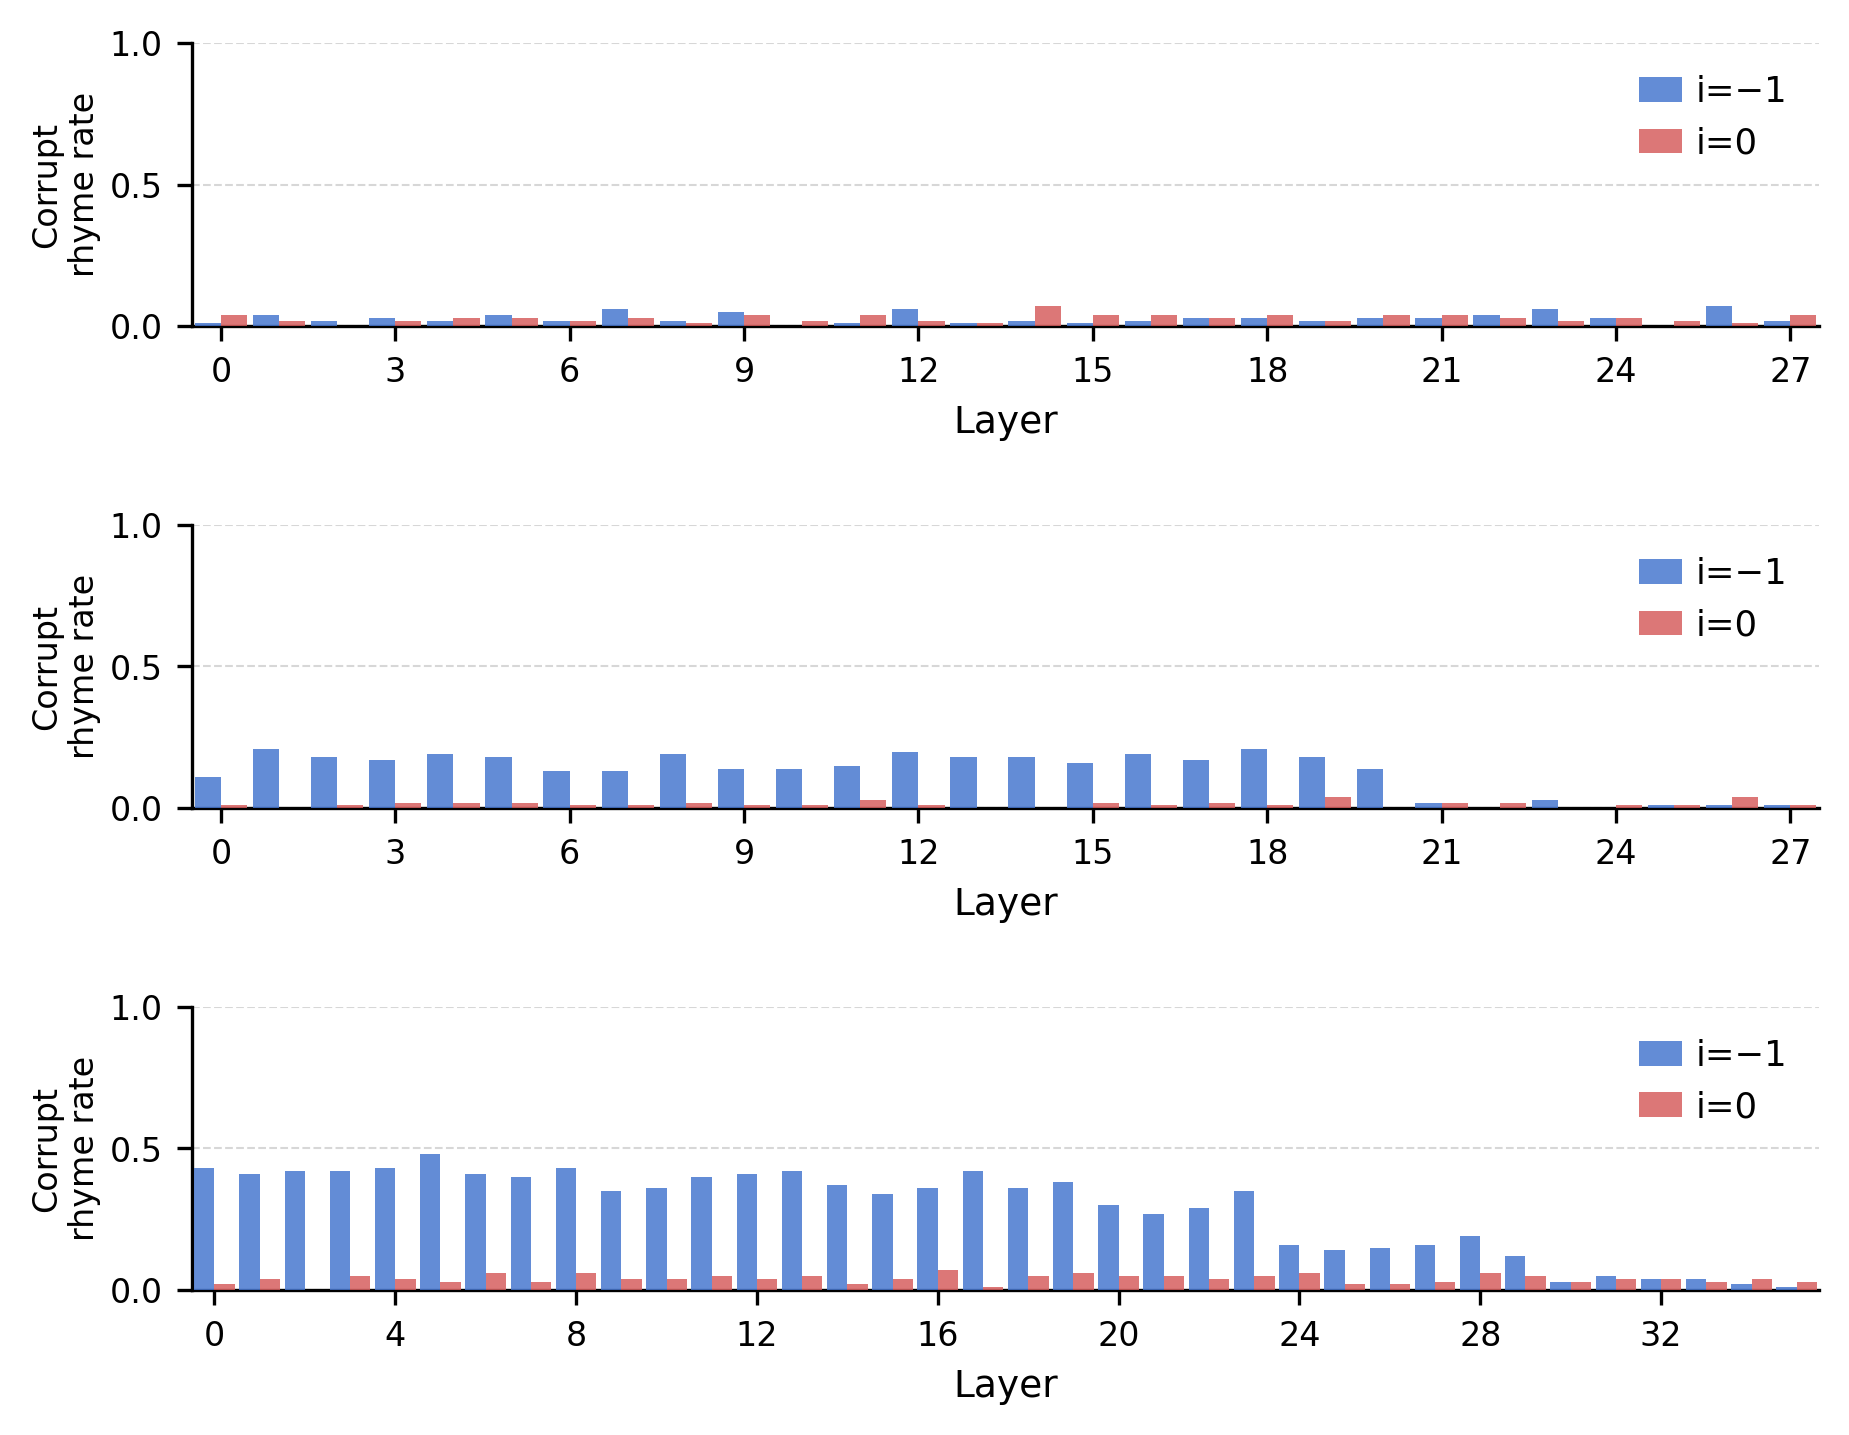
\includegraphics[width=\linewidth]{media/results-patching/appendix_patching_Qwen3_small.png}
    \caption{Per-layer activation patching, Qwen3 0.6B--4B.}
    \label{fig:appendix-patch-qwen3-small}
\end{figure}

\begin{figure}[H]
    \centering
    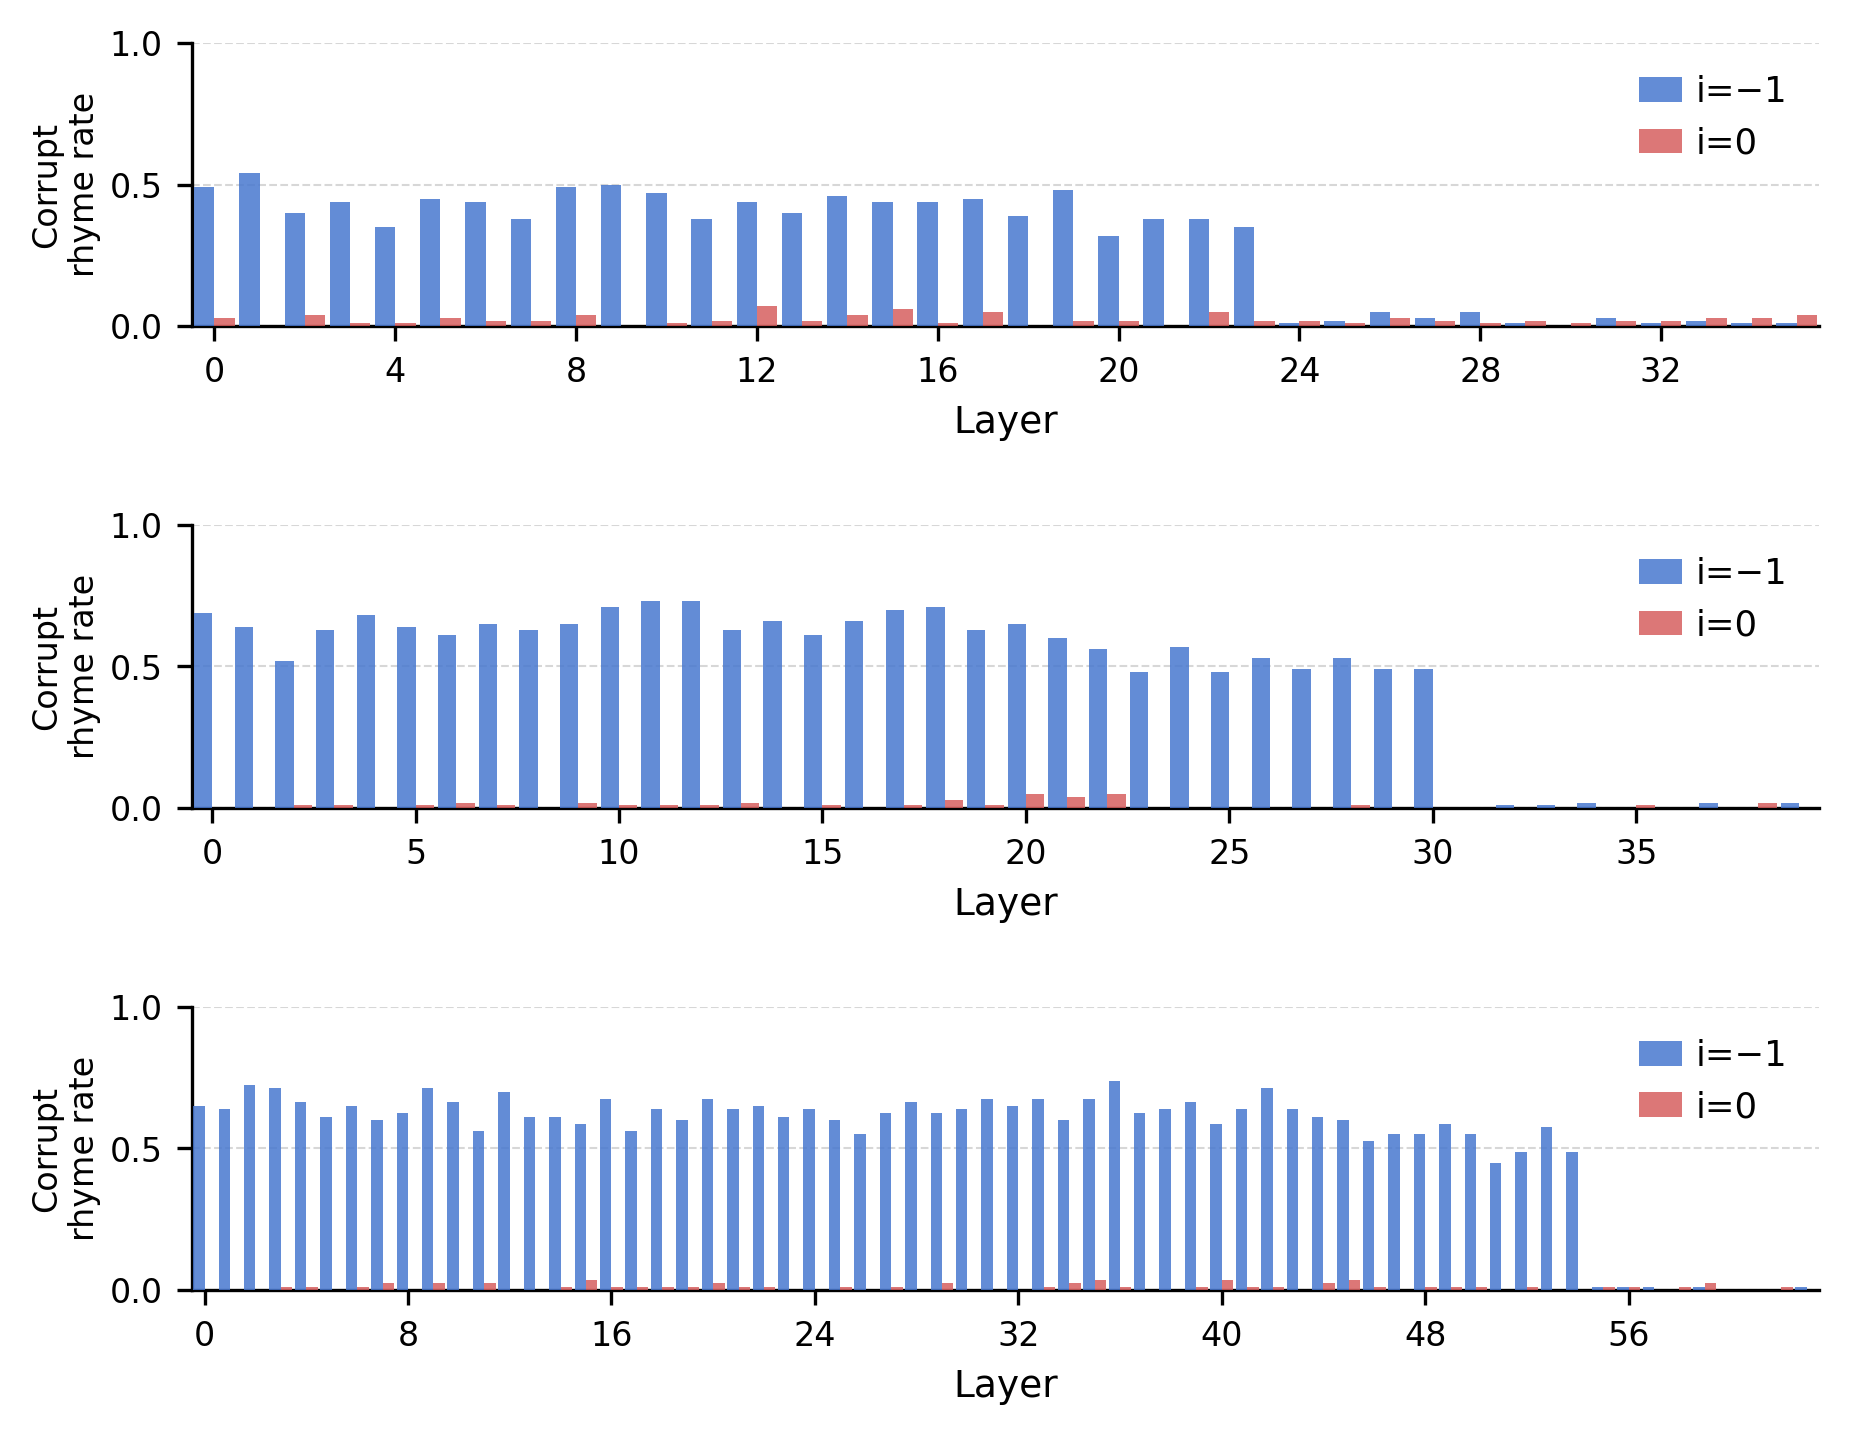
\includegraphics[width=\linewidth]{media/results-patching/appendix_patching_Qwen3_large.png}
    \caption{Per-layer activation patching, Qwen3 8B--32B.}
    \label{fig:appendix-patch-qwen3-large}
\end{figure}

\begin{figure}[H]
    \centering
    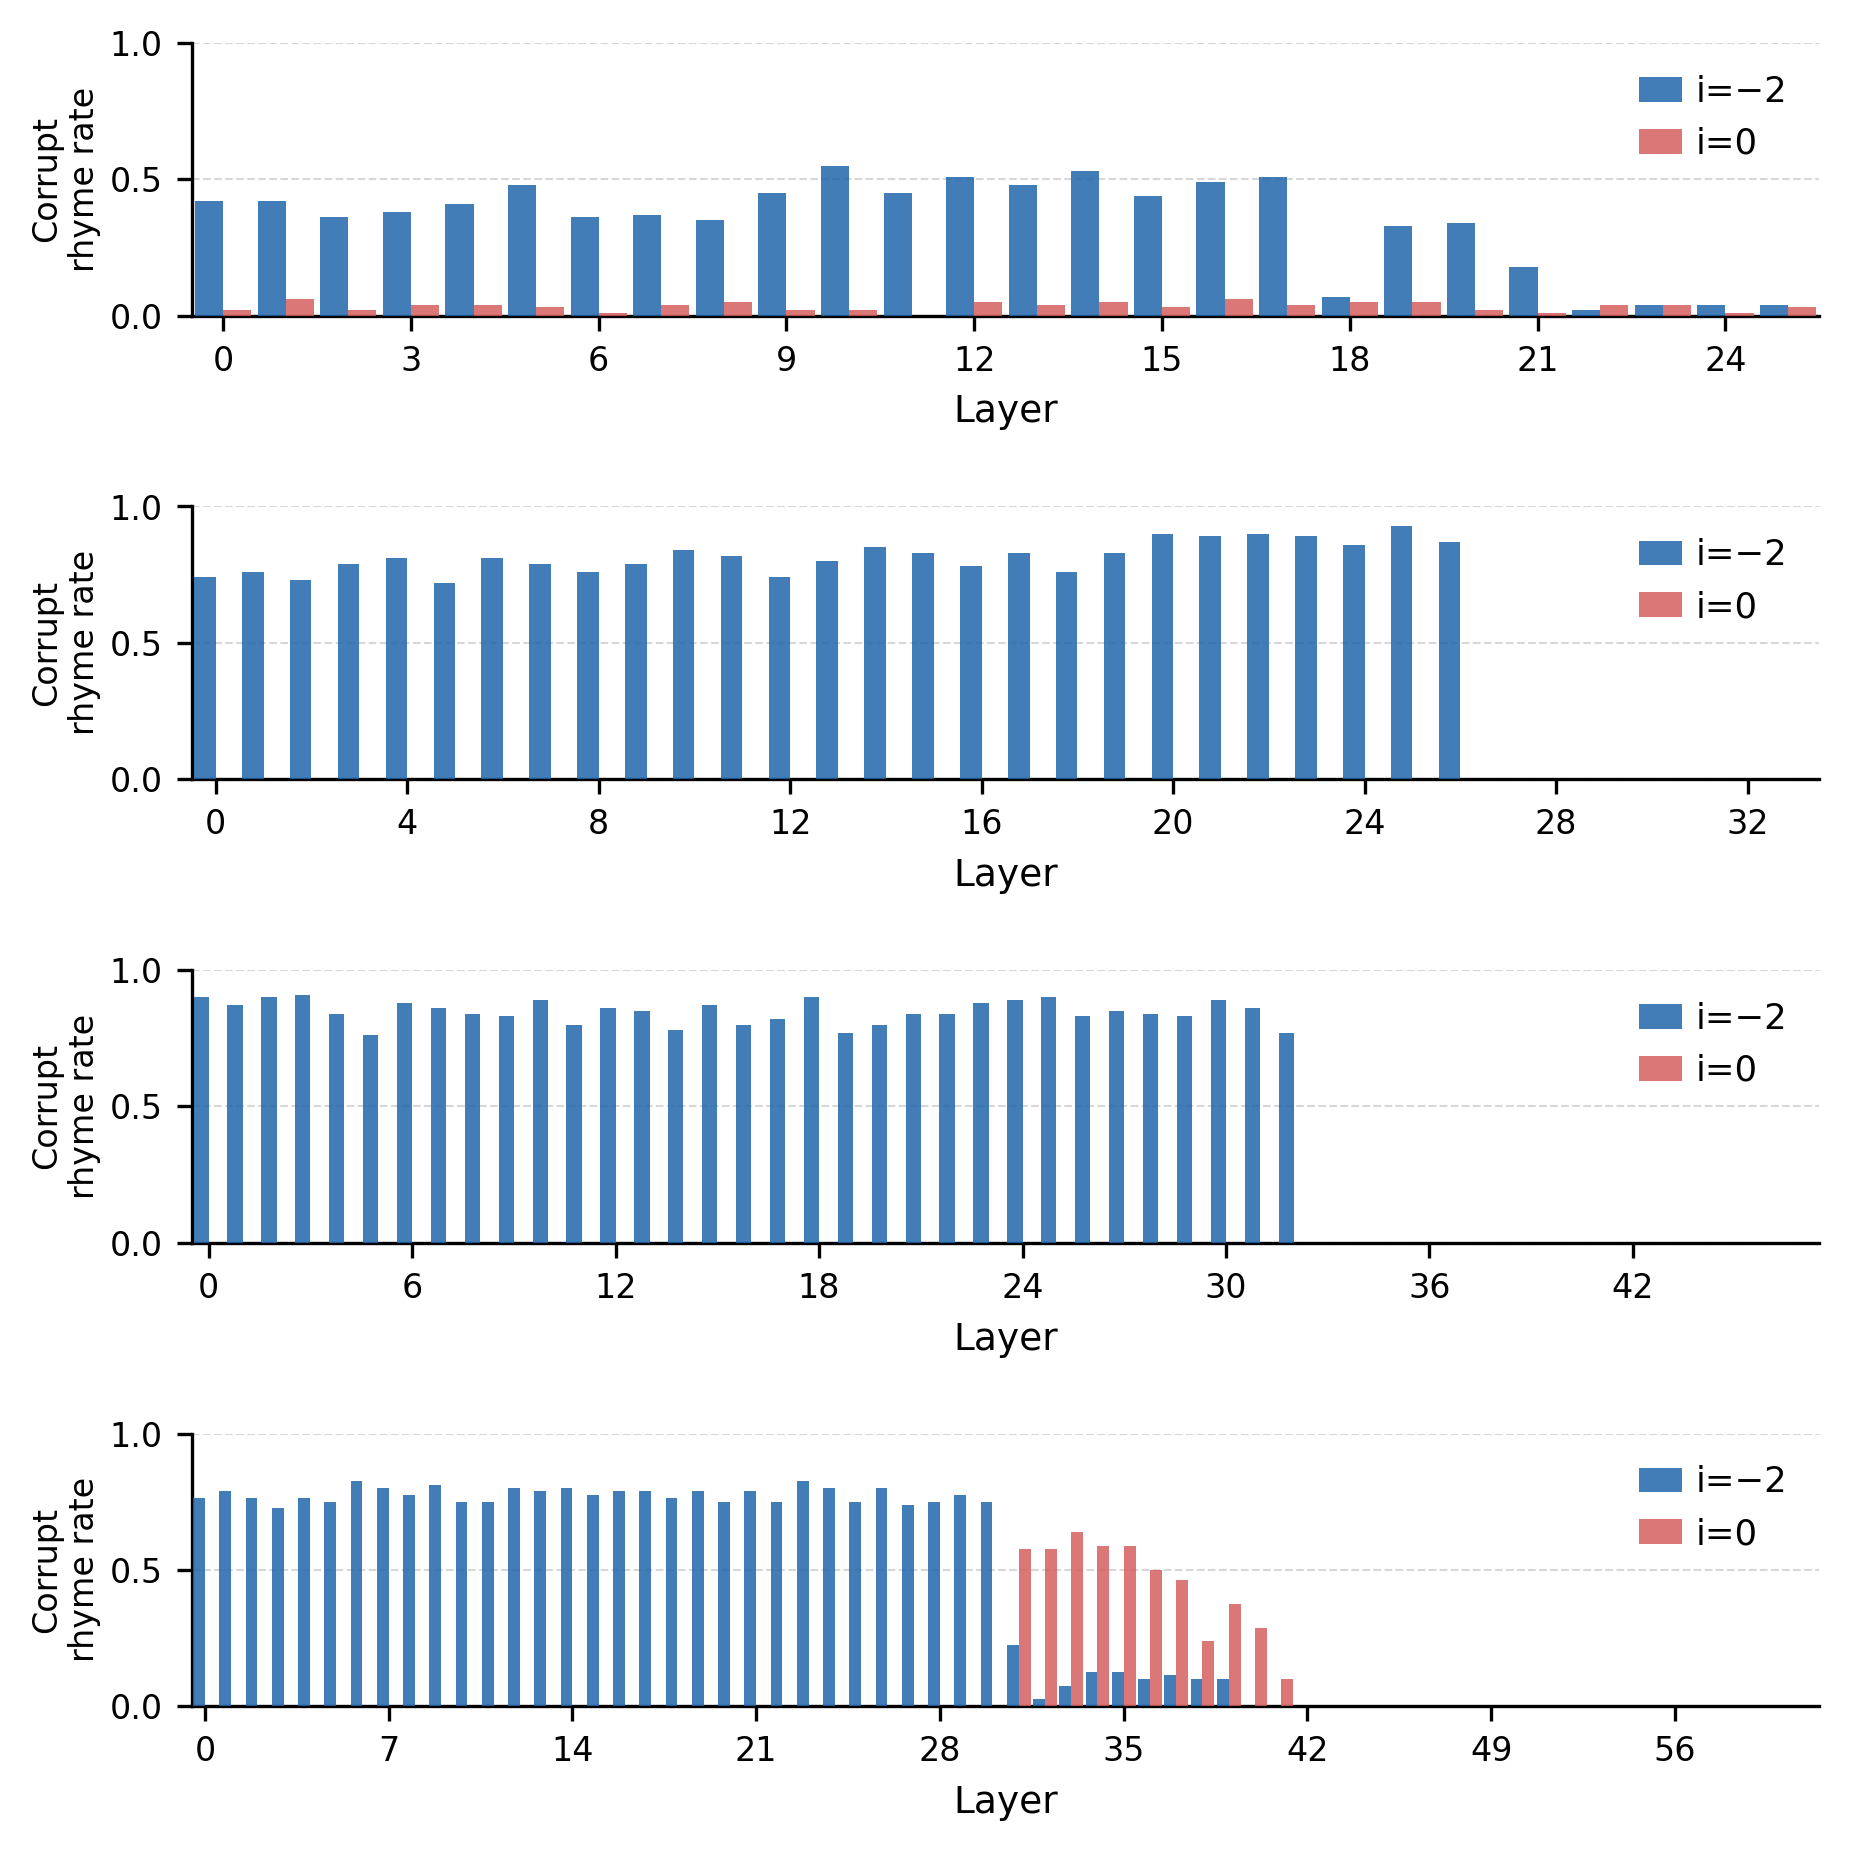
\includegraphics[width=\linewidth]{media/results-patching/appendix_patching_Gemma3.png}
    \caption{Per-layer activation patching, Gemma-3 1B--27B.}
    \label{fig:appendix-patch-gemma3}
\end{figure}

\begin{figure}[H]
    \centering
    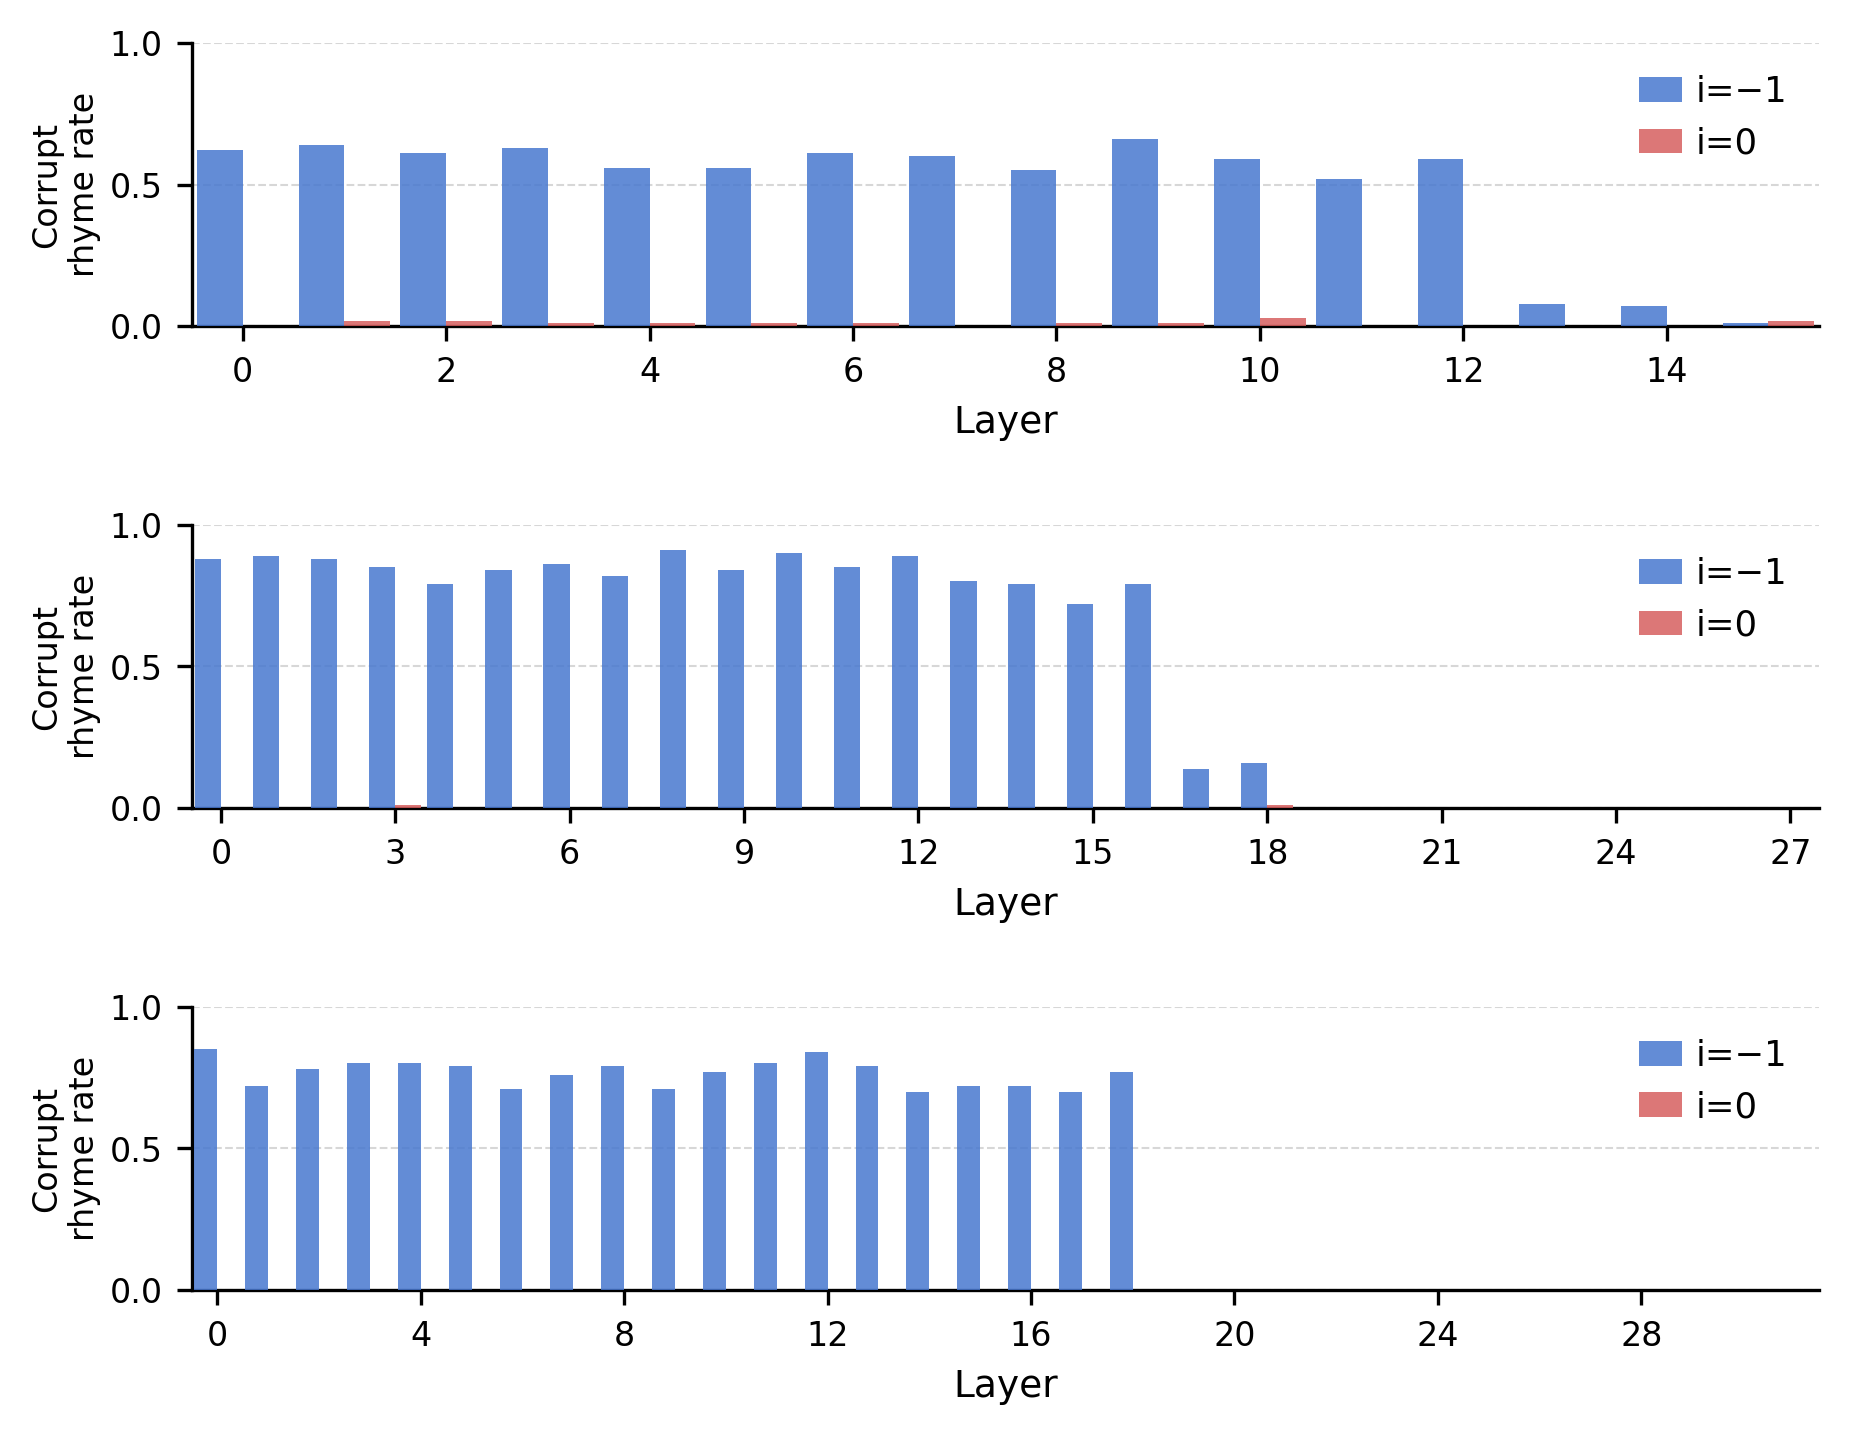
\includegraphics[width=\linewidth]{media/results-patching/appendix_patching_Llama3.png}
    \caption{Per-layer activation patching, Llama-3 1B--8B.}
    \label{fig:appendix-patch-llama3}
\end{figure}

\subsection*{Full Position Sweep}
\label{sec:additional-patching-sweep}

Figures~\ref{fig:appendix-sweep-qwen3-small}--\ref{fig:appendix-sweep-llama3} extend the analysis to all six swept positions ($i=-2$ through $i=+3$). Positions $i>0$ correspond to generated tokens, steered using the vector computed at $i=0$. Across all models and families, generated-token positions show near-zero corrupt rhyme rates, confirming that causal influence on rhyme selection does not persist into the generated sequence. The dominance of the last word token over the newline at all non-Gemma-3-27B scales is visible throughout.

\begin{figure}[H]
    \centering
    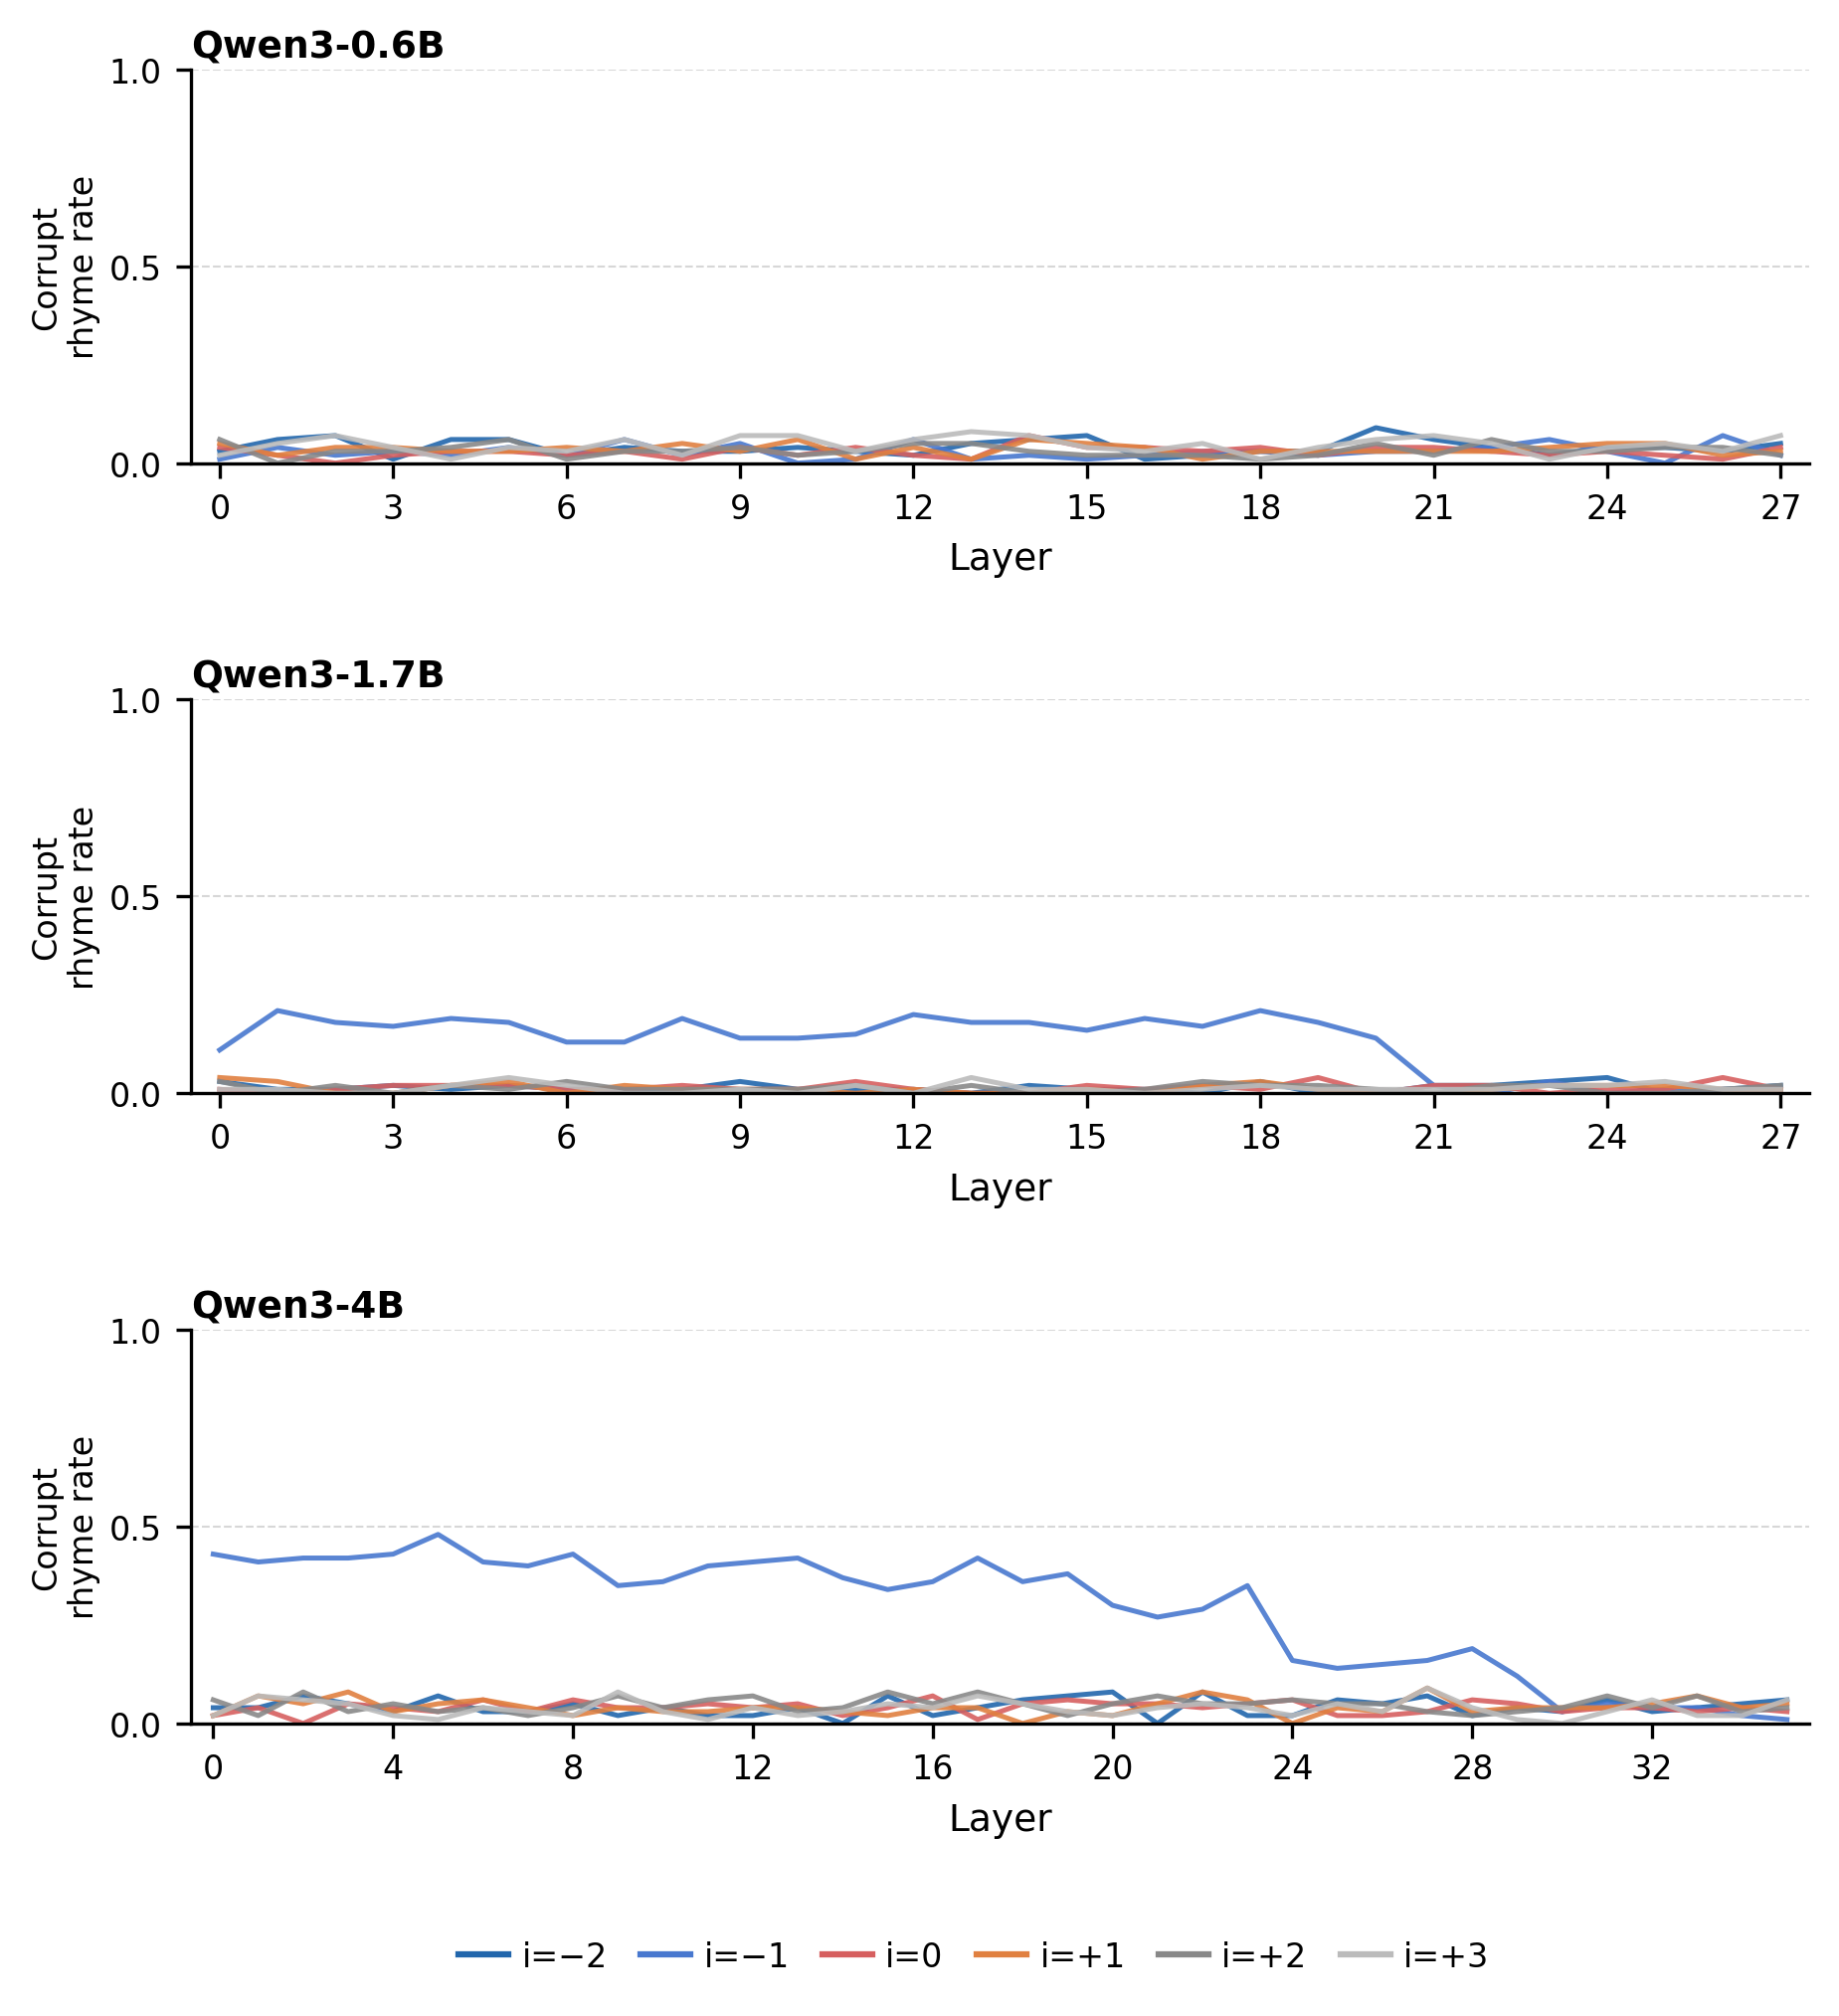
\includegraphics[width=\linewidth]{media/results-patching/appendix_sweep_Qwen3_small.png}
    \caption{Full position sweep, Qwen3 0.6B--4B.}
    \label{fig:appendix-sweep-qwen3-small}
\end{figure}

\begin{figure}[H]
    \centering
    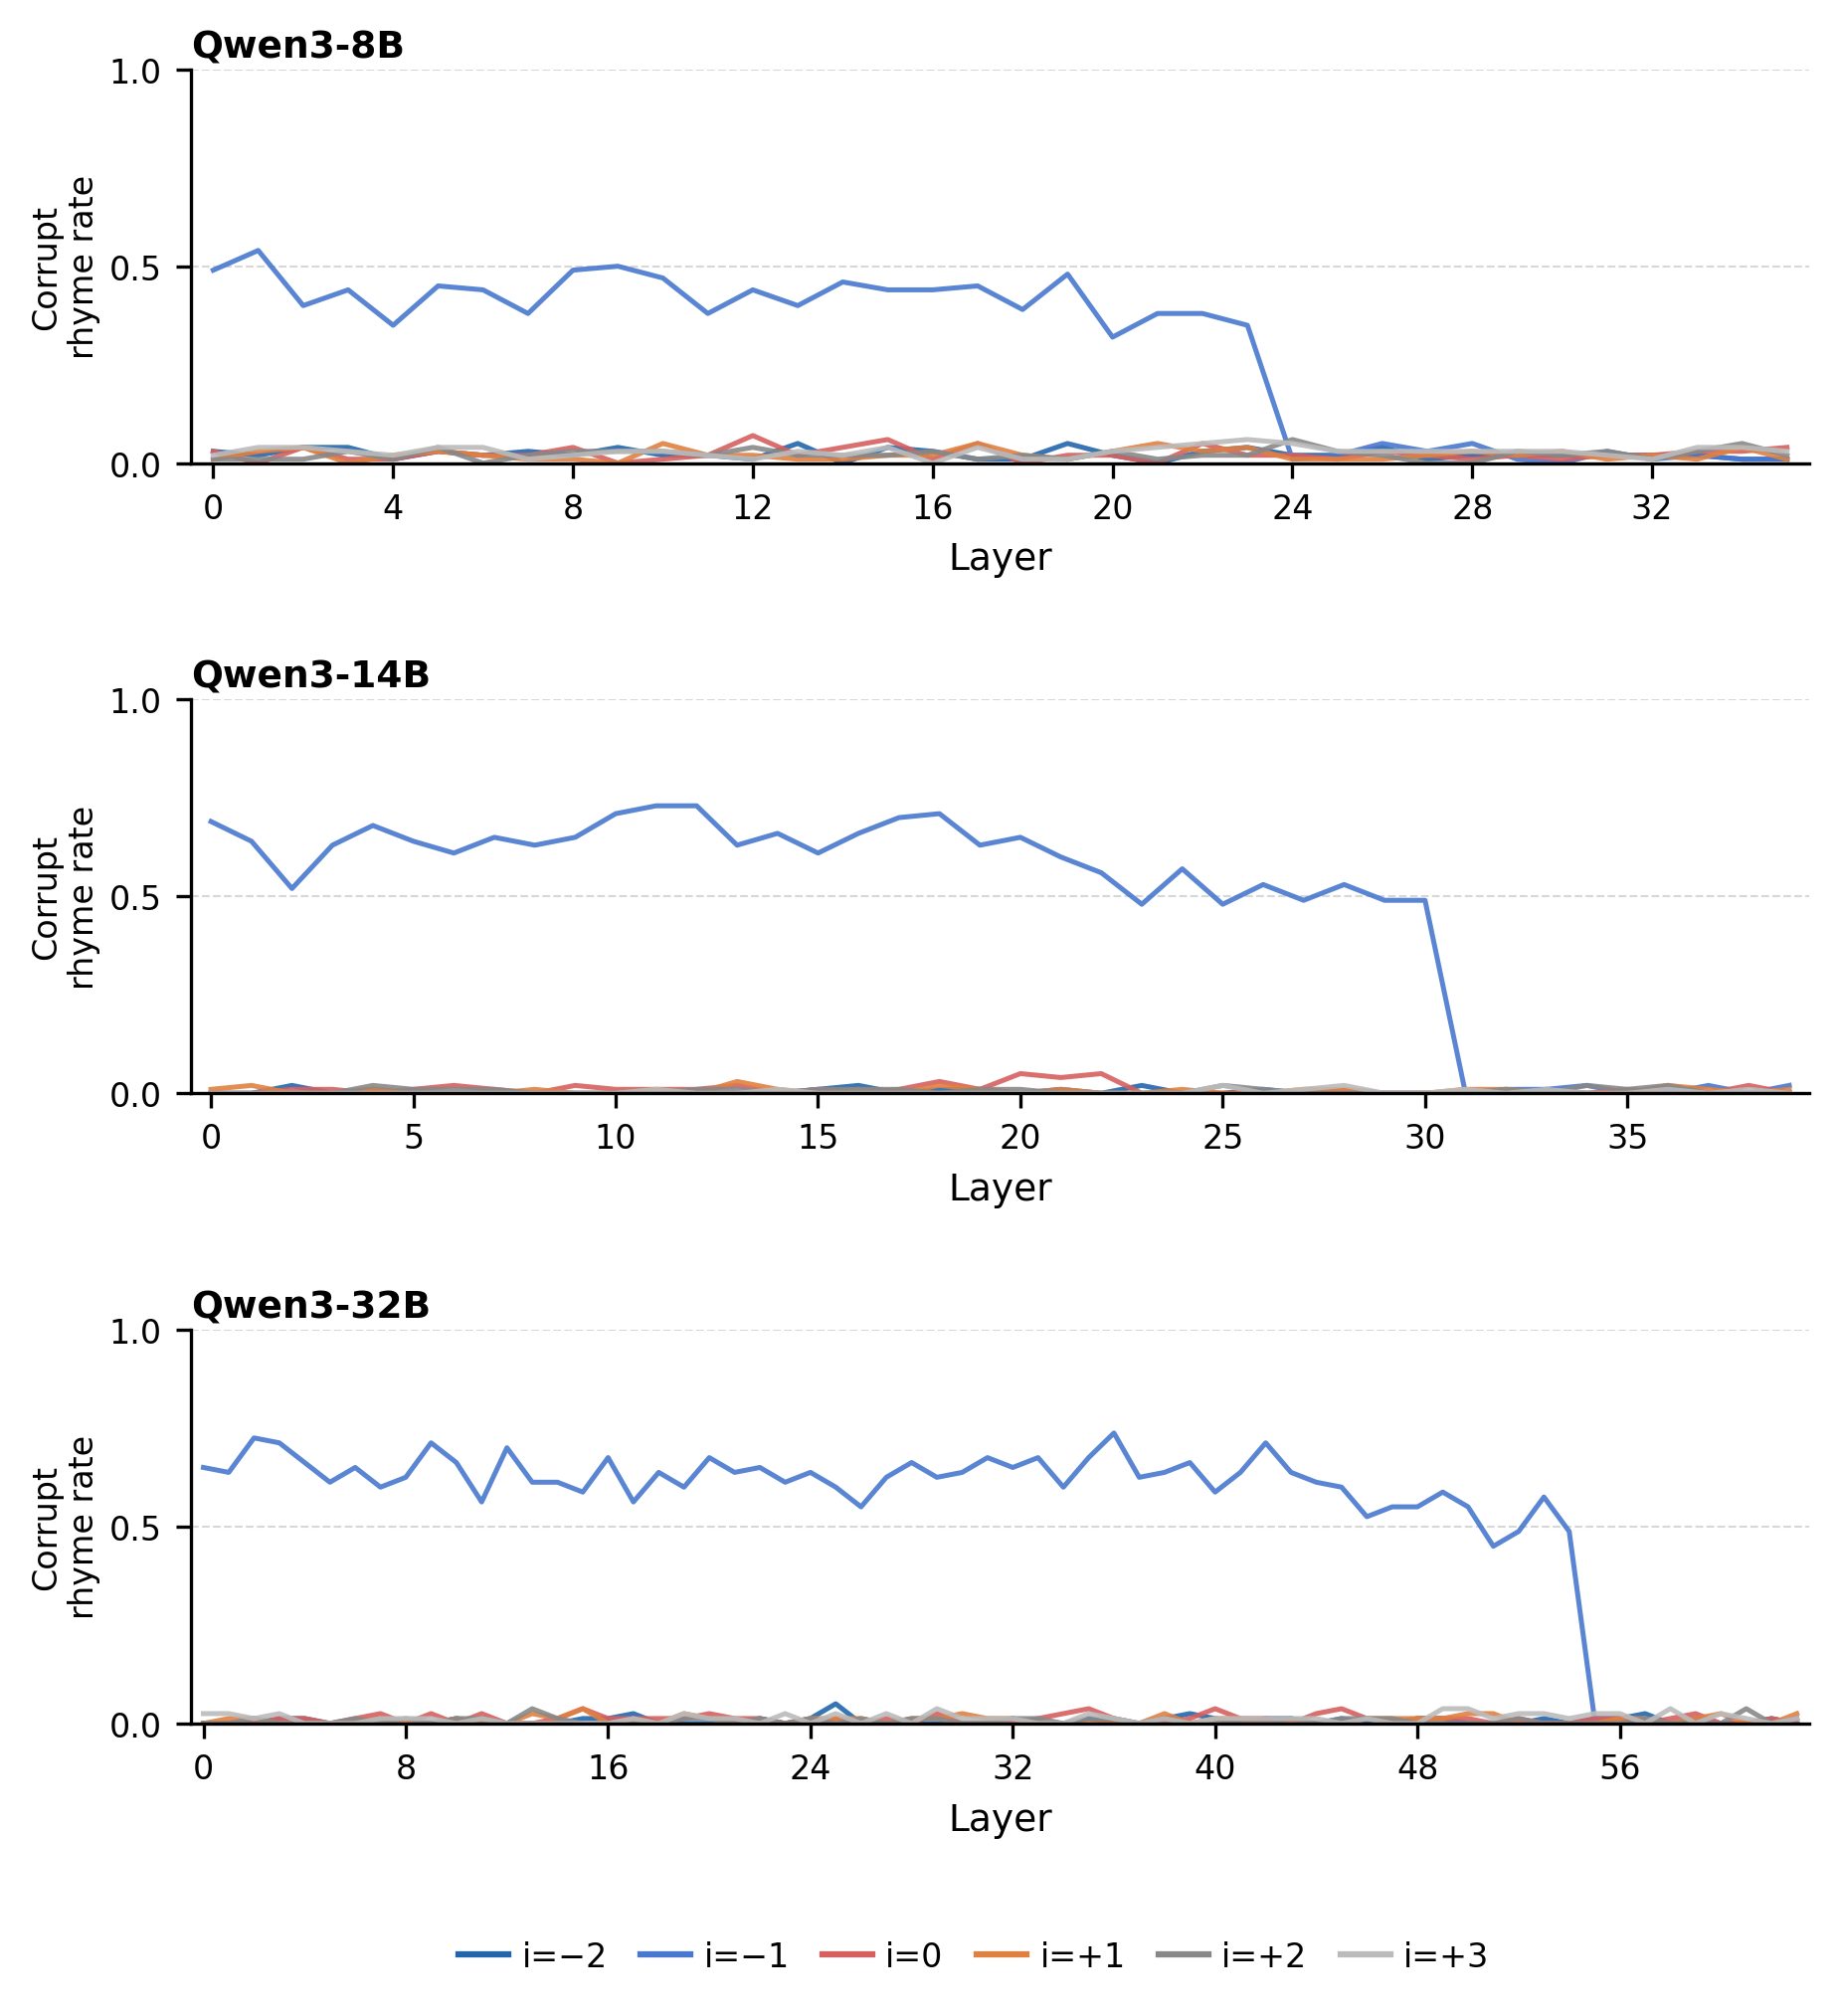
\includegraphics[width=\linewidth]{media/results-patching/appendix_sweep_Qwen3_large.png}
    \caption{Full position sweep, Qwen3 8B--32B.}
    \label{fig:appendix-sweep-qwen3-large}
\end{figure}

\begin{figure}[H]
    \centering
    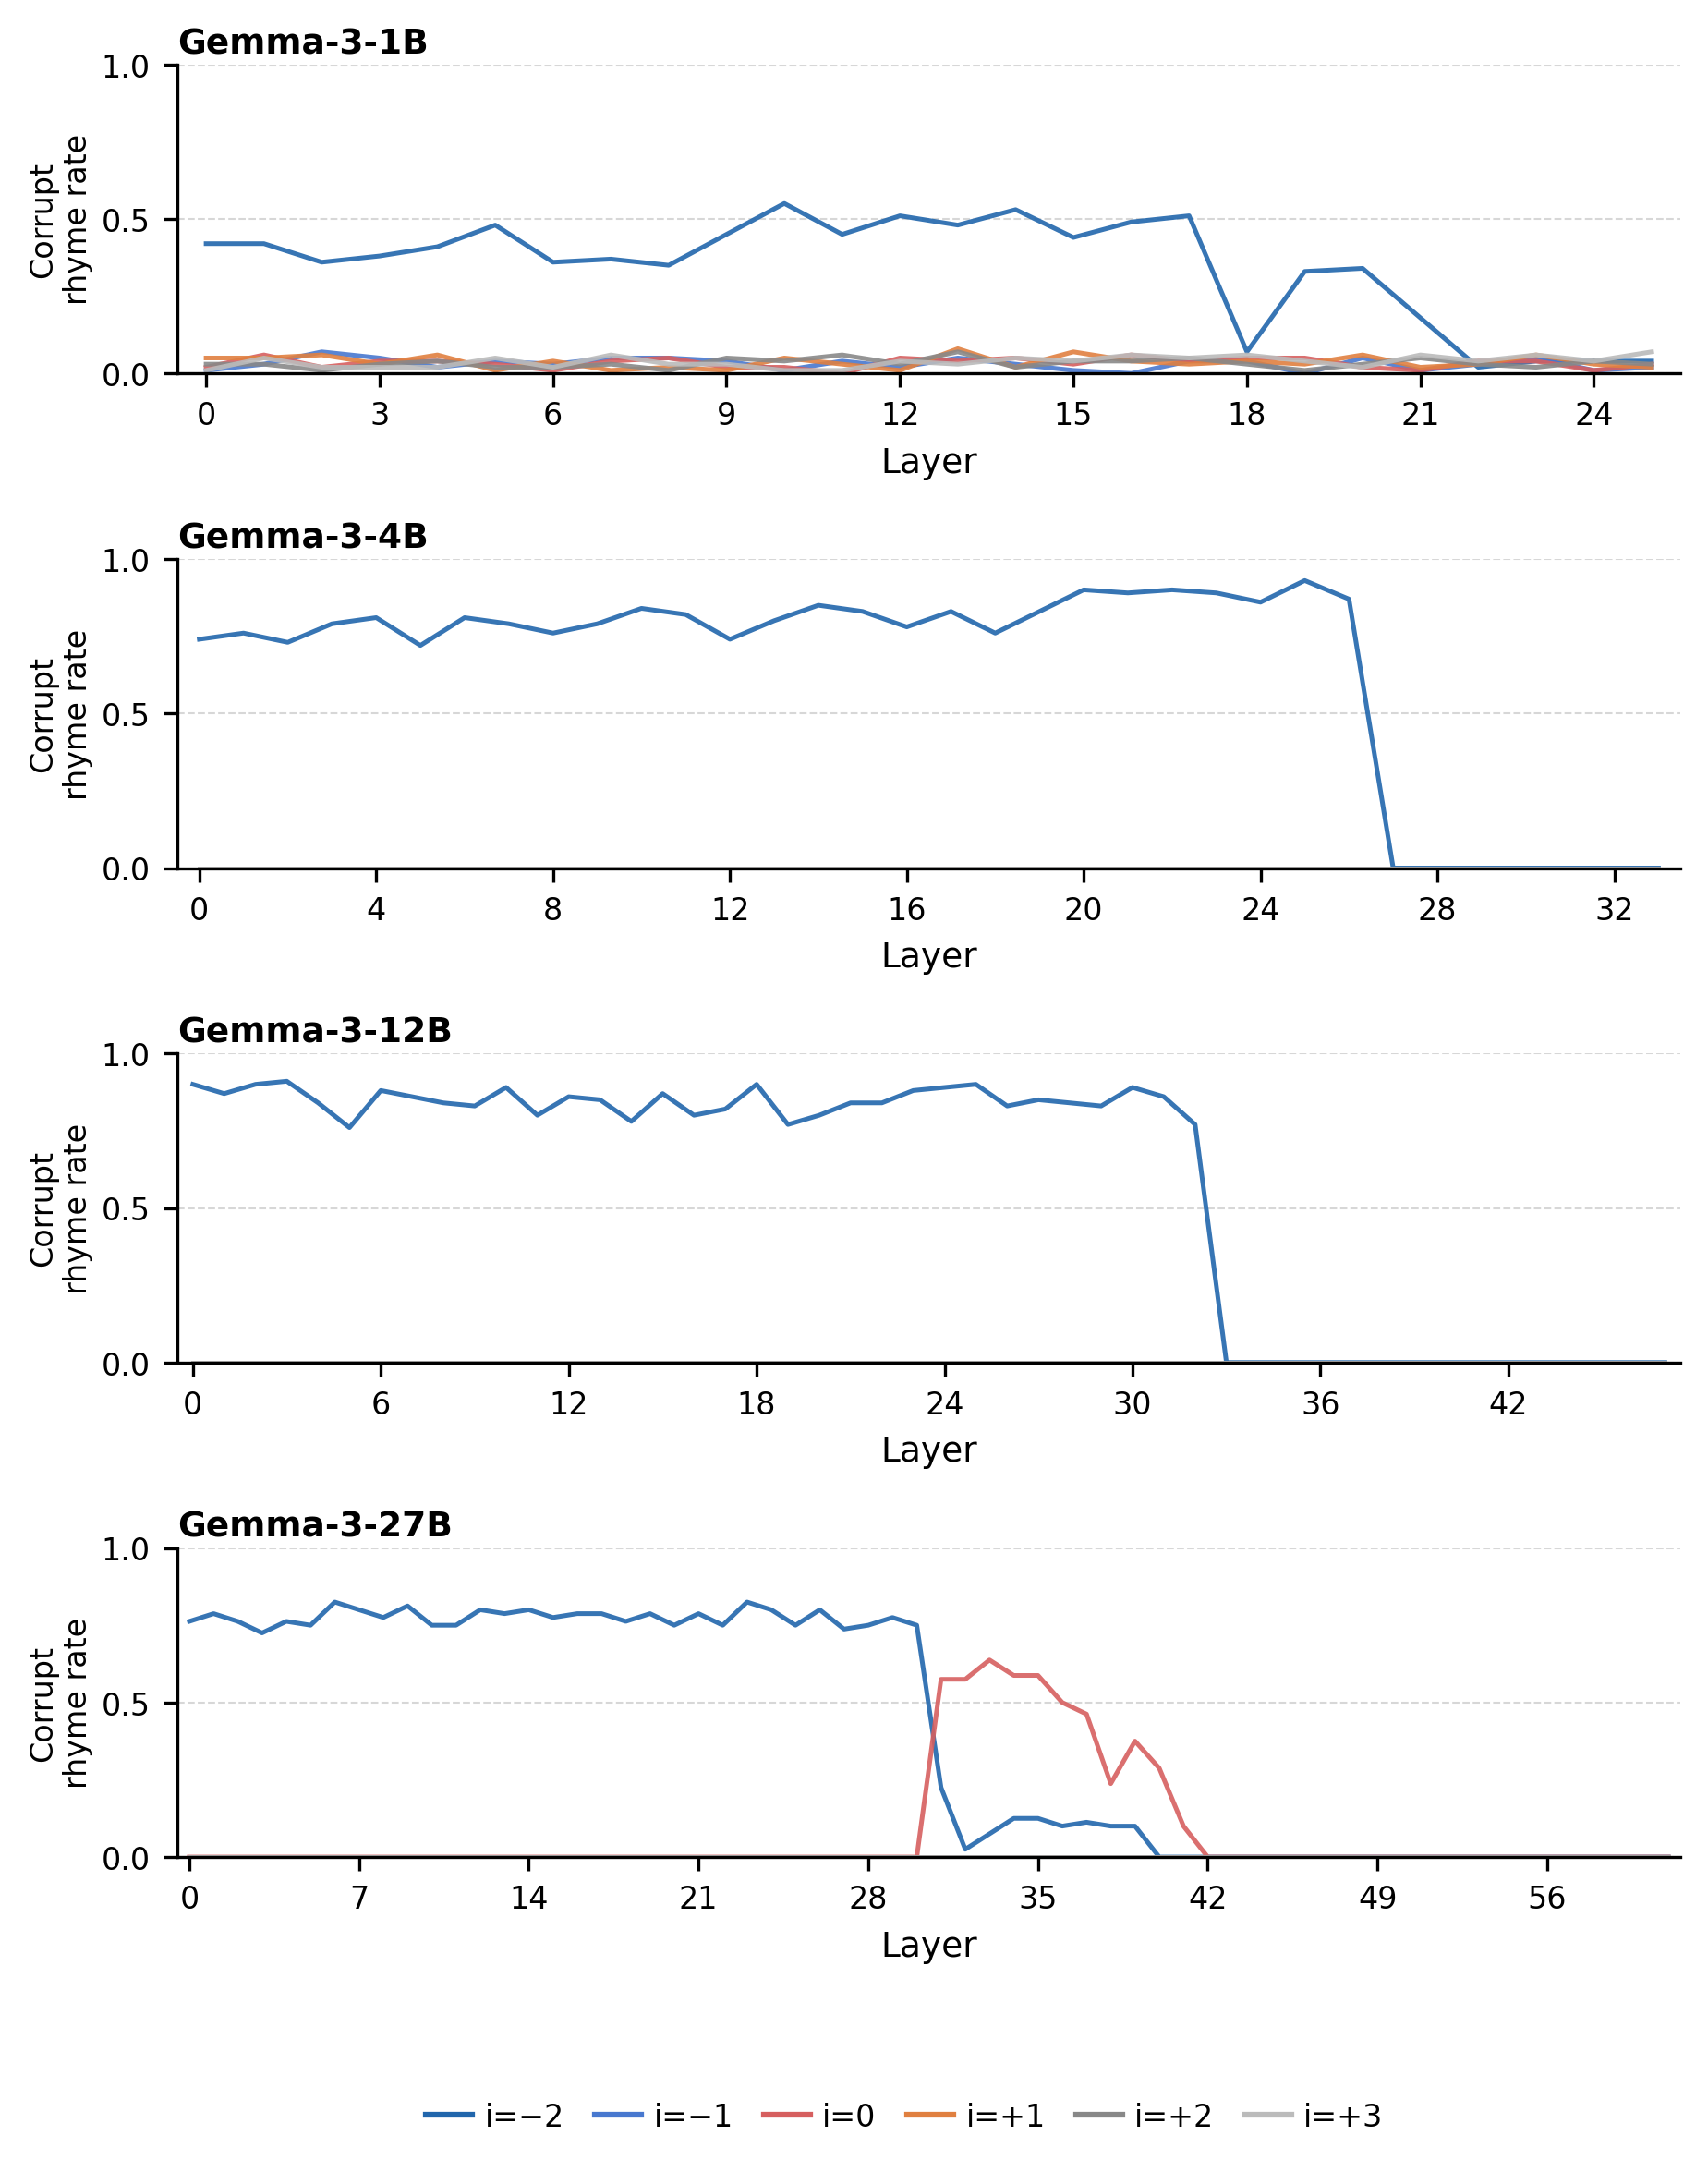
\includegraphics[width=\linewidth]{media/results-patching/appendix_sweep_Gemma3.png}
    \caption{Full position sweep, Gemma-3 1B--27B.}
    \label{fig:appendix-sweep-gemma3}
\end{figure}

\begin{figure}[H]
    \centering
    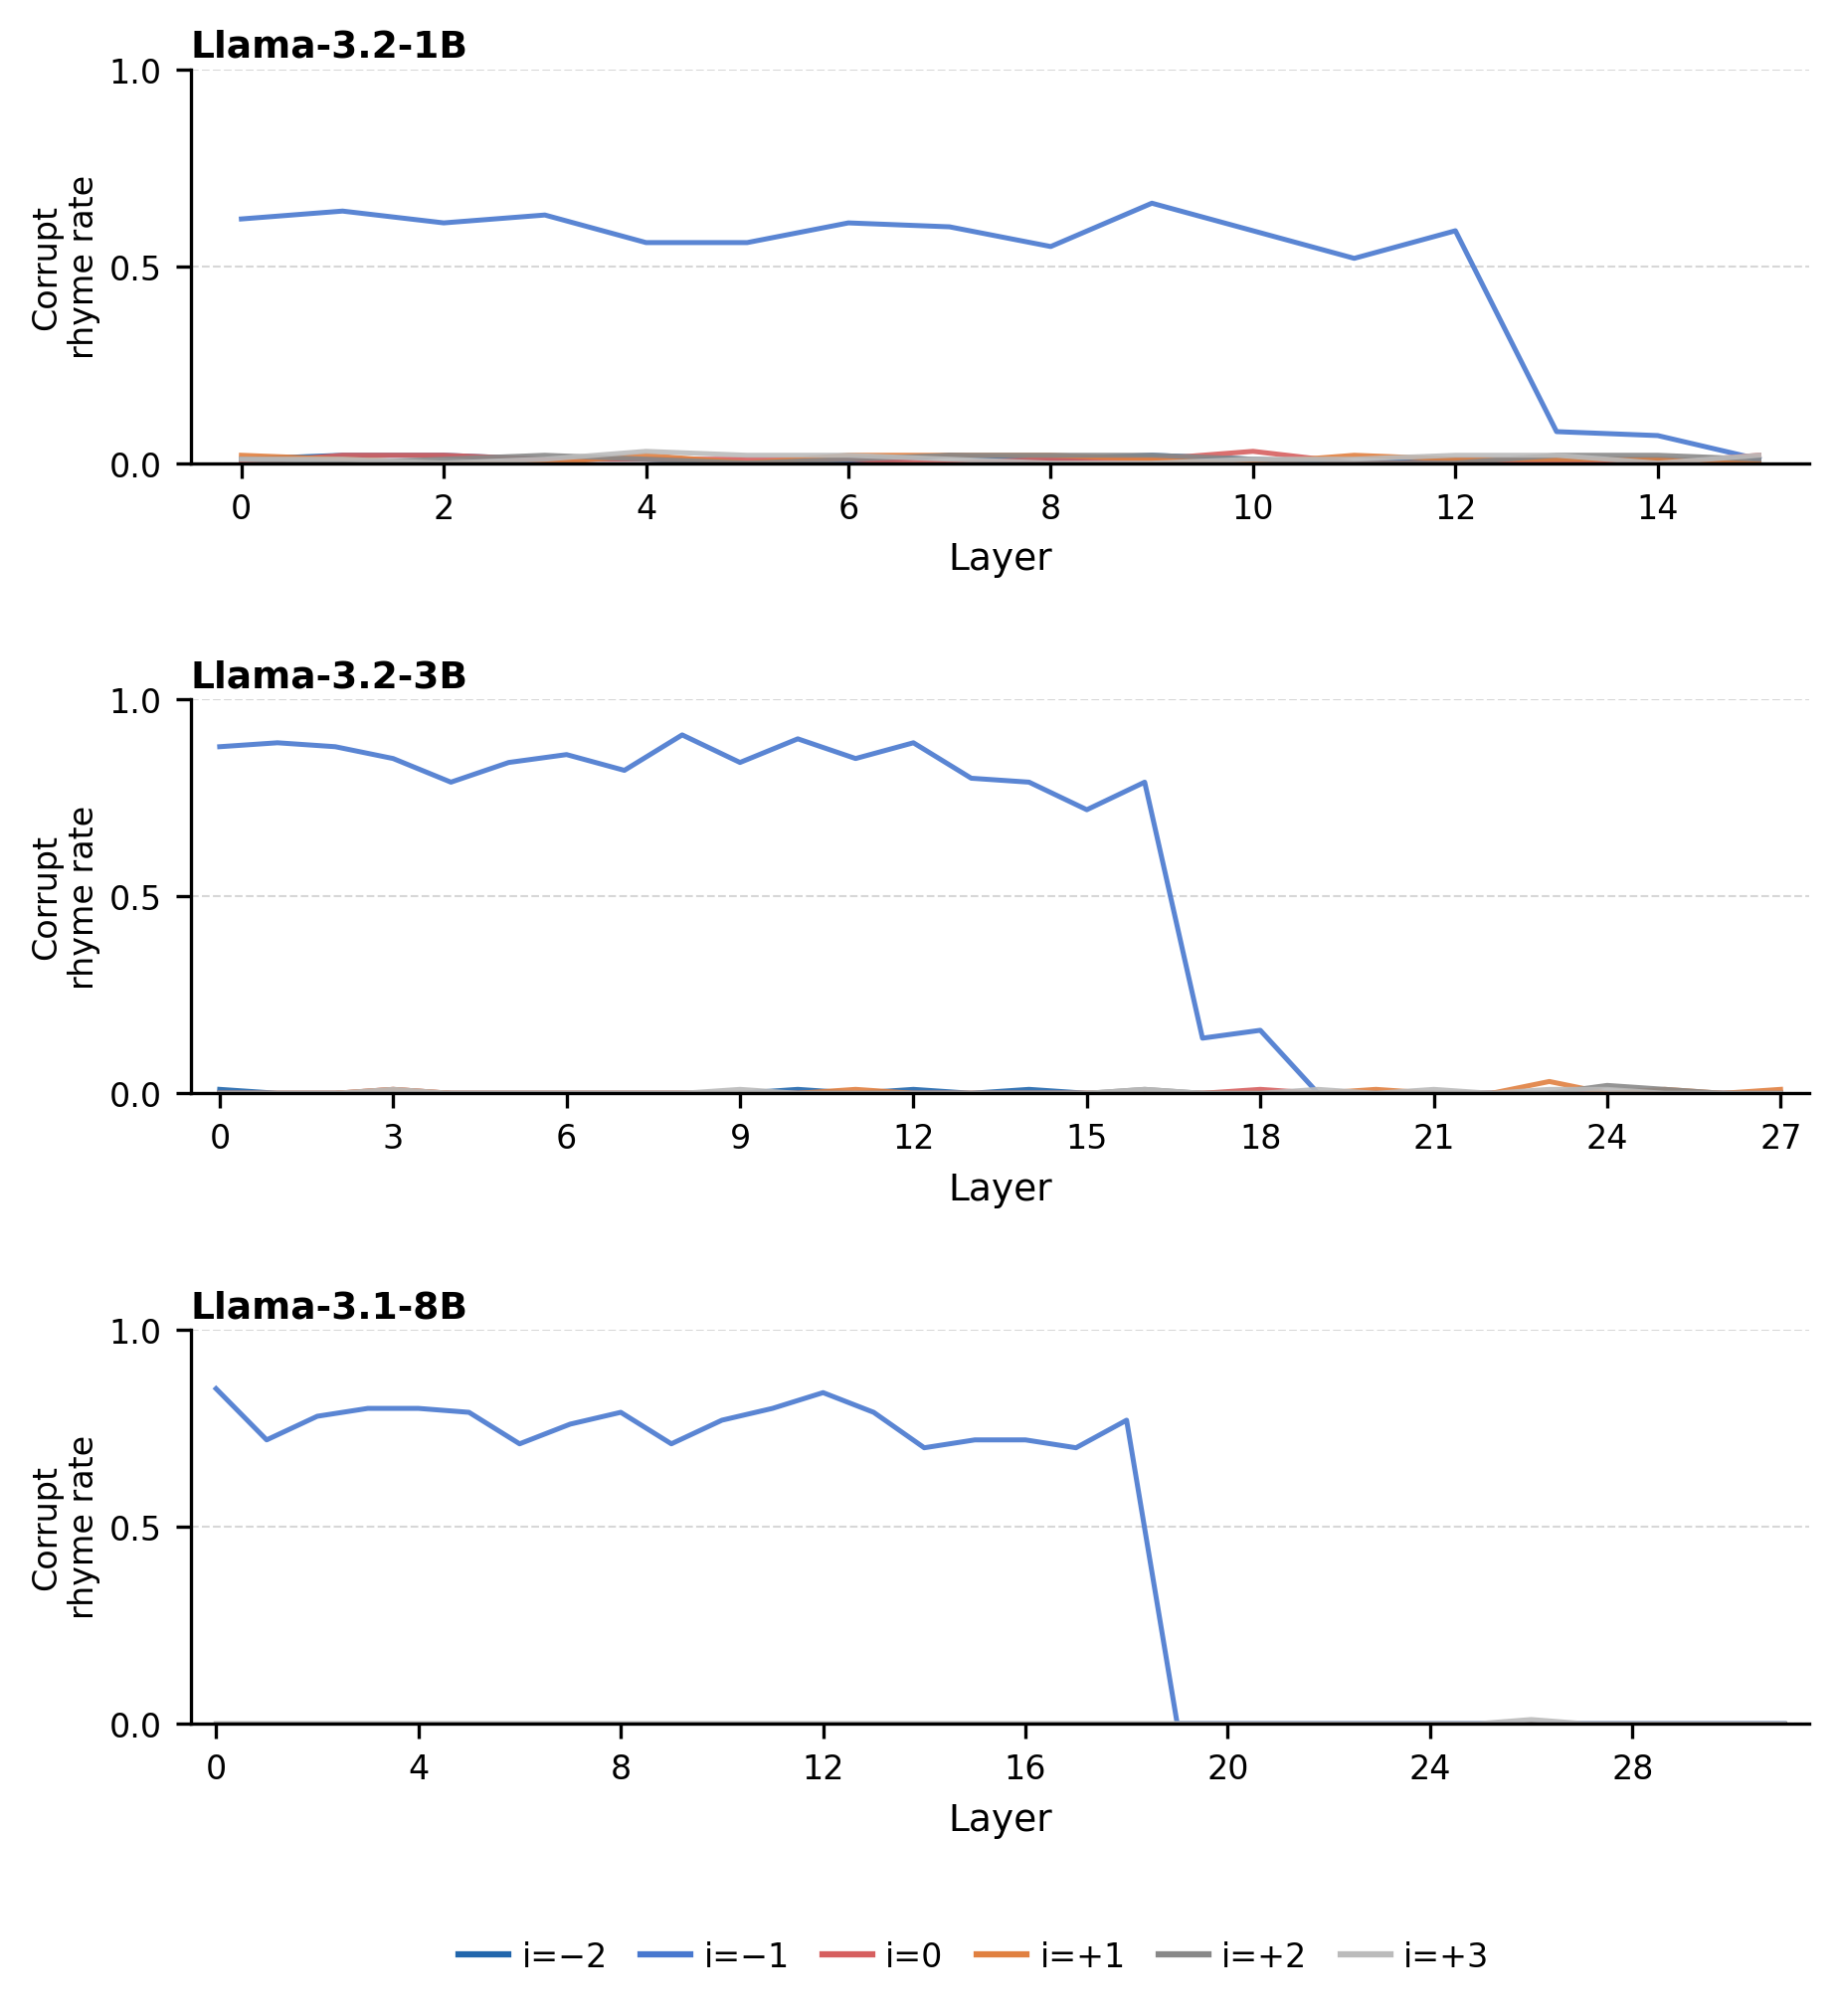
\includegraphics[width=\linewidth]{media/results-patching/appendix_sweep_Llama3.png}
    \caption{Full position sweep, Llama-3 1B--8B.}
    \label{fig:appendix-sweep-llama3}
\end{figure}

\subsection*{Prompt Pairs}

For each pair, we show the clean prompt, the corrupt prompt, and an example patched completion
where activation patching was successful in steering the rhyme scheme.

\begin{tabularx}{\linewidth}{@{}l>{\raggedright\arraybackslash}X@{}}
\textbf{Pair 1: doom / dread, $\ell=10$, $i=-1$:} & \\
Clean:   & \texttt{A rhyming couplet:\textbackslash n The empty house was filled with silent doom,\textbackslash n when suddenly they} \\
Corrupt: & \texttt{A rhyming couplet:\textbackslash n The empty house was filled with silent dread,\textbackslash n when suddenly they} \\
Patched: & \texttt{when suddenly they heard a creaking bed.}
\end{tabularx}

\medskip
\begin{tabularx}{\linewidth}{@{}l>{\raggedright\arraybackslash}X@{}}
\textbf{Pair 2: bliss / joy, $\ell=1$, $i=-2$:} & \\
Clean:   & \texttt{A rhyming couplet:\textbackslash n The children laughed in bliss,\textbackslash n until they all} \\
Corrupt: & \texttt{A rhyming couplet:\textbackslash n The children laughed in joy,\textbackslash n until they all} \\
Patched: & \texttt{until they all became a toy.}
\end{tabularx}

\medskip
\begin{tabularx}{\linewidth}{@{}l>{\raggedright\arraybackslash}X@{}}
\textbf{Pair 3: dark / night, $\ell=0$, $i=-2$:} & \\
Clean:   & \texttt{A rhyming couplet:\textbackslash n She wandered home alone into the dark,\textbackslash n and then she} \\
Corrupt: & \texttt{A rhyming couplet:\textbackslash n She wandered home alone into the night,\textbackslash n and then she} \\
Patched: & \texttt{and then she saw a strange and eerie light.}
\end{tabularx}

\medskip
\begin{tabularx}{\linewidth}{@{}l>{\raggedright\arraybackslash}X@{}}
\textbf{Pair 4: grief / pain, $\ell=2$, $i=-1$:} & \\
Clean:   & \texttt{A rhyming couplet:\textbackslash n I never knew the depth of such grief,\textbackslash n as though the} \\
Corrupt: & \texttt{A rhyming couplet:\textbackslash n I never knew the depth of such pain,\textbackslash n as though the} \\
Patched: & \texttt{as though the sky had lost its rain.}
\end{tabularx}

\medskip
\begin{tabularx}{\linewidth}{@{}l>{\raggedright\arraybackslash}X@{}}
\textbf{Pair 5: fright / fear, $\ell=1$, $i=-1$:} & \\
Clean:   & \texttt{A rhyming couplet:\textbackslash n She felt a sudden sense of fright,\textbackslash n and hoped that} \\
Corrupt: & \texttt{A rhyming couplet:\textbackslash n She felt a sudden sense of fear,\textbackslash n and hoped that} \\
Patched: & \texttt{and hoped that someone would appear.}
\end{tabularx}

\begin{figure}[H]
    \centering
    \begin{subfigure}{0.49\linewidth}
        \centering
        \subcaption[]{Qwen3-32B}
        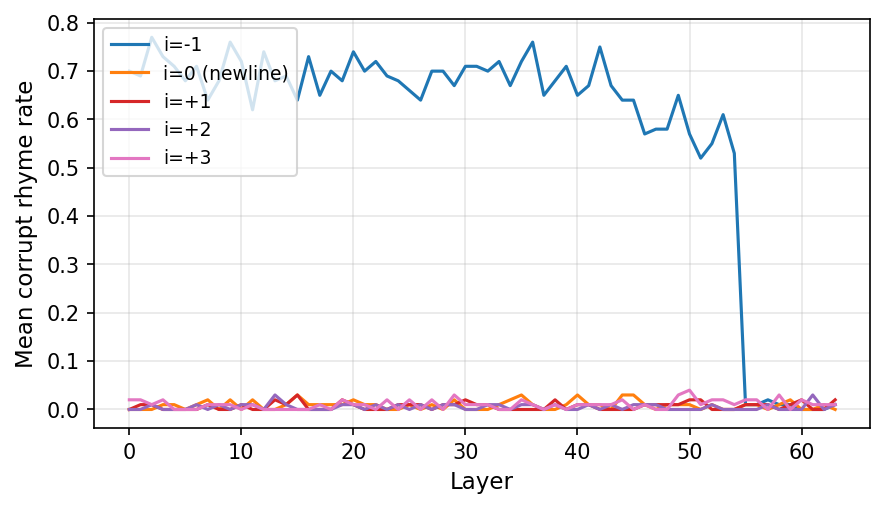
\includegraphics[width=\linewidth]{media/results-patching/qwen3_32b_aggregate_overlay.png}
    \end{subfigure}
    \begin{subfigure}{0.49\linewidth}
        \centering
        \subcaption[]{Gemma-3-27B}
        
\includegraphics[width=\linewidth]{media/results-patching/gemma3_27b_aggregate_overlay.png}
    \end{subfigure}
    \caption{Corrupt rhyme rate across all six swept token positions, averaged over 5
    prompt pairs ($N=100$). For Gemma-3-27B, the comma token at $i=-1$ is near zero
    throughout, confirming the handoff is specific to the newline token.}
    \label{fig:patching-all-positions}
\end{figure}

\end{document}
